\documentclass[11pt,a4paper, twoside]{book}

\usepackage{amsmath}
\usepackage{float}
\usepackage{geometry}
\usepackage{graphicx}
\usepackage{subfig}
\usepackage{xspace}
\usepackage{tcolorbox}
\usepackage{physics}
\usepackage{listings}
\usepackage{utfsym}


\usepackage[hidelinks]{hyperref}
\hypersetup{
    colorlinks=false
}

\usepackage[sorting=none, style=nature]{biblatex}
\addbibresource{stuff/bibliography.bib}

\usepackage{cleveref}





\newcommand{\routine}[2]{\section{#1}\label{sec:#2} \input{characterization/#2}} 

\newcommand{\experimentrecap}[4]{
\begin{tcolorbox}[colback=blue!10!white, colframe=blue!50!white, title=Experiment recap: \textbf{#1}, coltitle=black]
    \begin{description}
        \item[Scope:]\hfill\break #2.
        \item[Parameters to extract:]\hfill\break #3.
        \item[Brief description:]\hfill\break #4.
    \end{description}
\end{tcolorbox}
}

\newcommand{\fluxexperimentrecap}[4]{
\begin{tcolorbox}[colback=red!10!white, colframe=red!50!white, title=Experiment recap: \textbf{#1}, coltitle=black]
    \begin{description}
        \item[Scope:]\hfill\break #2.
        \item[Parameters to extract:]\hfill\break #3.
        \item[Brief description:]\hfill\break #4.
    \end{description}
\end{tcolorbox}
}

\newcommand{\RFSoC}{\textbf{RFSoC4x2}\xspace}
\newcommand{\ZCU}{\textbf{ZCU111}\xspace}

\newcommand{\Qibo}{\texttt{Qibo}\xspace}
\newcommand{\Qibolab}{\texttt{Qibolab}\xspace}
\newcommand{\Qibocal}{\texttt{Qibocal}\xspace}
\newcommand{\Qibosoq}{\texttt{Qibosoq}\xspace}
\newcommand{\Qick}{\texttt{Qick}\xspace}

\newtheorem{theorem}{Theorem}

\newcommand{\pd}[2]{\frac{\partial #1}{\partial #2}}
\newcommand{\pipulse}{$\pi$-pulse\xspace}
\newcommand{\pipulses}{$\pi$-pulses\xspace}
\newcommand{\pihpulse}{$\pi/2$-pulse\xspace}
\newcommand{\pihpulses}{$\pi/2$-pulses\xspace}




\begin{document}

\newgeometry{margin=1in}

\begin{titlepage}

\begin{center}
    {\LARGE{Università degli studi di Milano Bicocca}}\\
    {\hspace{1cm}}\\
    {\small{Dipartimento di Fisica "Giuseppe Occhialini"}}\\
    {\hspace{1cm}}\\
    {\small{Corso di Laurea magistrale in Fisica}}
\end{center}

\vspace{0.2cm}

\begin{figure}[H]
    \centering
    
\includegraphics[width=0.4\textwidth]{stuff/logo.png}
\end{figure}

\vspace{0.5cm}


\begin{center}
    {\textbf{\LARGE {Qubit characterization and calibration on a RFSoC-based control system}}} \\ \vspace{0.4cm}
    {\textbf{\large {The long journey from the hardware setup to a possible quantum sensing application, developing an economic alternative to commercial control devices}}}
\end{center}

\vspace{1.8cm}

% probably I should add titles...
\begin{minipage}[t]{0.47\textwidth}
	{Supervisor:\\ \large{\bf Andrea Giachero}}
	\vspace{0.5cm}
	{\\External supervisor:\\ \large{\bf Stefano Carrazza}}
	\vspace{0.5cm}
	{\\Co-supervisor:\\ \large{\bf Matteo Borghesi}}
	\vspace{0.5cm}
	{\\External co-supervisor:\\ \large{\bf Javier Serrano}}
\end{minipage}
\hfill\begin{minipage}[t]{0.47\textwidth}\raggedleft
	{Candidate:\\ \large{\bf Rodolfo Carobene}}
	\vspace{0.5cm}
	{\\Student Number: \\\large{\bf 838092}}
\end{minipage}

\vspace{30mm}

\centering{\large{\bf ACADEMIC YEAR 2022/2023 }}
\end{titlepage}

\restoregeometry

\clearpage % end title page
\begingroup
  \pagestyle{empty}
  \null
  \newpage
\endgroup

% Fine frontespizio




\frontmatter
\chapter{Abstract}

Quantum computing has attracted significant interest from its early beginnings, even when there were no physical implementations of quantum computers yet.
The proposal and development of algorithms (such as those by Shor and Grover), that are theoretically more efficient than what can be designed with classical computers, have led to significant progress in this field over the last decade.

These early discoveries have led to an intensification of research and development, aided by the active involvement of private companies, such as Google and IBM, which, within a few years, have invested in new technologies and built computers efficient enough to claim the achievement of a "Quantum Primacy".
%
Although these advancements have yielded noticeable results, current computers are still not precise enough to be practically useful.
Indeed, we are in what is referred to as the "Noisy Intermediate-Scale Quantum" (NISQ) era, where quantum computers exist, but are too noisy to support quantum algorithms without encountering errors.\\
%
For this reason, after years of research focusing on increasing the number of qubits (the quantum computing equivalent of classical bits), current research is shifting its focus toward designing and building more reliable and efficient individual qubits.
%
In order to achieve this goal, research is working simultaneously in multiple directions: experimenting with various types of qubits (superconducting, trapped ions, etc.), trying to enhance the highly delicate qubit fabrication processes, and improving the methods for qubit control and operation.\\
%
My thesis work is part of the research concerning the last point: Quantum Control, specifically for superconducting qubits.

A superconducting qubit can be represented as a LC circuit where the classical inductance is replaced by a non-linear inductance obtained with a Josephson junction.
This junction exploit the phenomenon of superconductivity to create a non-harmonic Hamiltonian, allowing the separation of the first two states (those used for computation) from the others.
The qubit is then coupled to a classical resonator, described by a harmonic Hamiltonian, which is used for readout.
%
All transition frequencies of this system, which can be precisely studied within the framework of cQED (circuit Quantum ElectroDynamics)~\cite{Blais2021}, are typically on the order of GHz.
%
By applying voltage pulses at these frequencies, it is possible to read the state of the qubit and modify it as desired.
%
However, synthesizing the required pulses is itself a technological challenge, as typical Digital to Analog Converters (DACs) reach at most hundreds of MHz, requiring up/down-conversion schemes that necessitate the use of additional equipment.
This complicates the experimental setup and introduce additional sources of noise into a system that is highly sensitive to external disturbances.
%
All parameters describing the pulses are precisely calibrated to maximize the qubit's performance (relaxation time $T_1$, dephasing time $T_2$, accuracy), and even minor variations can significantly affect coherence times or lead to leakage outside the computational space.
This requires the use of specialized instruments.

Several companies have developed proprietary tools for the synthesis and definition of these pulses.
However, these tools are often expensive, and researchers are frequently constrained in signal quality due to typical up/down-conversion schemes.
Additionally, each instrument is controlled using different software and programming languages, which complicates integration into a unified control and readout framework.

A recent, more versatile, and cost-effective alternative is the use of RFSoC boards (Radio Frequency System on Chip).
These boards are a specific type of FPGA (Field Programmable Gate Arrays) composed of programmable integrated circuits, all connected on a single board, which also incorporates several high-performance RF components.
The most notable feature of RFSoC boards is their ability to synthesize GHz pulses with great precision and full control~\cite{Kalfus2020}, achieved through a technique known as Direct Digital Synthesis (DDS).\\
%
RFSoC boards, initially developed for communications purposes, have quickly become appealing also for quantum computing due to their synthesis capabilities and the inclusion of a single electronic board that houses a CPU, multiple high-performance DACs, and ADCs.
Additionally, since 2020, the Fermilab's \Qick project~\cite{Stefanazzi2022} has provided open-source firmware, enabling the programming of these FPGAs for qubit control and readout purposes.

In my thesis work, I utilized \Qick as a foundation to develop \Qibosoq, an open-source software designed for the control and readout of superconducting qubits using RFSoC boards.
Additionally, \Qibosoq integrates RFSoC boards into the \Qibo framework, a high-level software platform that allows for the definition of quantum algorithms and circuits to be executed on hardware later on.

During my thesis period at the Technology Innovation Institute (TII) in Abu Dhabi, I focused on the characterization and calibration of qubits, by using \Qibosoq in conjunction with various RFSoC boards for the control of single fixed-frequency qubits (physically implemented with a single Josephson junction in a 3D cavity) and for the simultaneous control of multiple variable-frequency qubits (constructed with pairs of Josephson junctions coupled to planar resonators).

%
The characterization of qubits is a process that involves various experiments aimed at identifying all the key parameters specific to the qubit itself and to the resonant cavity to which it is coupled for readout.
These parameters are then used along with those obtained from additional calibration experiments to optimize the control of the qubit, making it suitable for applications in quantum computing or quantum sensing.
The sequence of the experiments required is typically composed of at least fifteen different experiments.
Each of these experiments involves the synthesis of specific pulse sequences and measurements aimed at optimizing one or more of the parameters that describe the system.\\
%
%For example, the Ramsey experiment, which allows the identification of the value of \(T_2\) (the decay constant describing the loss of coherence of the qubit system), is performed by synthesizing two consecutive pulses that take the qubit from a defined state (0-1) to a superposition and vice versa, using an operation described by \(\frac{1}{\sqrt{2}}\begin{pmatrix}1 & 1 \\ i & i \end{pmatrix}\).
%The two pulses are separated by a variable delay, and a relative phase of \(\pi/2\) is added to the second pulse.
%
%This process enables the examine, as a function of the delay between the two pulses, the typical dephasing decay that occurs following the first pulse.
%The pulses must be synthesized at the characteristic frequency of the qubit, and even small deviations can manifest as oscillatory precessions in the qubit state.
%For this reason, this procedure can also be used to precisely identify the qubit's transition frequency.

%Questo esempio illustra bene come un singolo esperimento possa risultare complesso da realizzare dal punto di vista sperimentale. 
%
%This example effectively illustrates how a single experiment can be quite complex to implement from an experimental perspective.
A system based on RFSoC boards, such as the one developed for this thesis, which does not require additional instruments beyond the board itself, can have a significant impact in simplifying the characterization and calibration operations.\\
Furthermore, it's important to note that once a qubit control system is developed, it can be used for a wide range of experiments beyond just calibration and characterization.

%
The work at TII has always been focused on quantum computing, meaning the use of qubits for the execution of quantum algorithms.
In this context, the developed system has already been used to run quantum machine learning algorithms aimed at estimating Parton Distribution Functions (PDFs) on qubits~\cite{Robbiati2023}.
%
However, in the future, it will also become an important tool for applications in quantum sensing, using qubits as particle detectors.

%
In particular, in 2021 the italian INFN (\textit{Istituto Nazione di Fisica Nucleare}) presented the Qub-IT project, which aims to use qubits for the search for dark matter, specifically for dark photons and axions~\cite{qubit_project}.
The fundamental idea behind Qub-IT is to couple a qubit to a cavity that, in resonance with potential dark matter particles, could induce the conversion of these particles into photons.
The various photons present in the cavity influence the coupled qubit, making it possible to measure the number of photons with high precision through a specific pulse sequence not too dissimilar from the one required in the previously mentioned Ramsey experiment.
%
In the project proposal document, one of the key points is the development of a qubit control and readout system using FPGAs that is precise, reliable, and scalable.
%
The work of my thesis represents an important step in this direction.

%
The thesis provides the theoretical elements of cQED necessary to understand how the control of superconducting qubits works.
It illustrates the experimental setup and hardware configuration required for the various RFSoC boards used, along with a detailed explanation of the unique features of RFSoC boards, including the synthesis and acquisition methods used to work directly in the GHz range. 
Additionally, the software \Qibosoq and \Qibolab, developed and used during the thesis work, are briefly introduced and commented upon.\\
%
The core of the thesis consists of a detailed explanation of the main experiments required for the characterization and calibration of single qubits and two-qubit gates.
Each experiment includes graphs to be obtained under ideal conditions, some real-world graphs, and solutions to some of the most common experimental problems.
This section is designed to potentially serve as a practical guide for the calibration and characterization of superconducting qubits.\\
%
Finally, the thesis concludes with two examples of possible applications of the developed control and readout system: the first in quantum machine learning (already tested on hardware), and the second in quantum sensing, related to the experiment for the search for dark matter.

\tableofcontents

\listoffigures \addcontentsline{toc}{chapter}{List of figures}
\begingroup
\let\clearpage\relax
\listoftables \addcontentsline{toc}{chapter}{List of tables}
\endgroup

%\chapter{Introduction}
%
%Quantum technologies are one of the newest and most thriving topic of research in modern physics.
%Although it is not clear how much they will change in the future and in which fields they will be more impactful, they are already providing interesting theoretical results, promising to achieve a \textit{computational capacity} higher than any possible supercomputer.
%
%Quantum technologies are being studied to revolutionize communication, security, chemistry, finance, fundamental physics and much more, but the question is now if and when the promised results will be delivered.
%The era we are currently living in is often referred to as the NISQ era (Noisy Intermediate-Scale Quantum devices), where no \textit{real} advantage has yet been taken from quantum computing.
%
%To answer this problem, the research is focusing on near-term applications (compatible with noisy devices), on non-computing applications (such as quantum sensing researches) and on optimizing the hardware and the control of the qubits.\\
%This thesis has some value for the last topic, since it adds tools for researches to control quantum devices.
%
%From the hardware point of view, there have been not many laboratories in the world with available qubits.
%This is because a qubit, in particular for a superconducting device, requires special instruments to work (such as cryostats) and extremely expensive hardware for readout and control of the qubit themselves.\\
%Despite the interest from manufacturers in commercializing expensive ready-to-run solutions, experimental laboratories still have to face the issue of acquiring instruments which are in continuous improvement in terms of firmware and software, therefore customers might even participate indirectly as co-developer by providing feedback, testing and waiting for improvements. This situation is not ideal because it increases the required manpower and time of a research team.\\
%This, along with the costs of the machinery, is without doubt slowing researchers, that have to rely on external hardware (such as the quantum computers offered by the IBMQ-Experience) over which they have little control.
%
%However, recently, Radio Frequency System on Chip (RFSoC) FPGAs (Field Programmable Gate Arrays) were proposed as a low-cost hardware alternative which provides flexible development of firmware and software related to quantum technologies. 
%Despite the complexity and required expertise for firmware development, the research community has already achieved open-firmware for quantum applications through the \Qick (Quantum Instrument Control Kit) project~\cite{Stefanazzi2022} under development at Fermilab National Laboratories.
%
%%In Italy, for the INFN QUB-IT project (see XX), FPGAs are stated as the to-go tool to reach full control over the qubits to be produced by the collaboration so \Qick is the natural and easiest way of managing them.
%While it is an outstanding project, however, \Qick is currently under development and even if it exposes all the tools to control a qubit, it does not simplify it particularly.\\
%A different, complementary, tool is under development at the Technology Innovation Institute (TII) of Abu Dhabi: \Qibolab.
%\Qibolab is a software that should provide a common and easy interface for researchers, to control quantum devices with an agnostic philosophy in respect to the control instruments, possibly supporting them all.
%It is also part of the \Qibo ecosystem, that gives a way of defining and simulating quantum algorithms from the circuit level.
%
%In order to write this thesis, I worked at TII laboratories with the objective of integrating the \Qick RFSoCs in \Qibolab through a new project called \Qibosoq project.
%Leveraging the \Qick, I created an open-source software that offers full control over superconducting qubits, making it easy to control them both for experiments at the low-pulse-level and for higher-level applications.\\
%The system was continuously tested in all the many characterization and calibration experiments that are required in order to make a qubit usable.
%
%The work done during the time at TII can be easily used by any laboratory that it is trying to implement the same qubit control solutions and has being presented to other researches through articles \cite{Efthymiou_2023}, YY.
%Moreover, the software developed has already been used for applications in the quantum machine learning field \cite{Robbiati2023}.
%
%The developed system is also of great relevance for INFN quantum sensing project QUB-IT~\cite{qubit_project}.
%The goal of the QUB-IT project is to realize an itinerant single-photon counter exploiting Quantum Non Demolition (QND) measurements and entangled qubits, in order to surpass current devices in terms of efficiency and low dark-count rates.
%Such a detector has direct applications in Axion dark-matter experiments (such as QUAX~\cite{quax_project}), which require the photon to travel along a transmission line before being measured.\\
%Among the outline of the project, the development of a full control system based on FPGAs is one of the critical in-itinere achievement and this thesis takes the first step in that direction.
%
%\vspace{1cm}
%
%In the first chapter of this thesis, I will provide the theoretical elements required to understand the importance of the search on the nature of Dark Matter, as well as all the needed elements of circuit QED to understand the functioning of a superconducting device such as a qubit.
%
%In the second chapter, I will talk about the experimental setup used for qubit control.
%This includes actual hardware such as the RFSoCs and the cryostat, but also the software developed as an important tool of coding experiments and controlling the FPGA.
%Moreover, a full in depth description of the peculiarity of a RFSoC system, in respect to the commercial alternatives will be provided.
%
%In the third chapter I will present, in detail, all the experiments required to characterize a qubit, so to find the parameters that describe it, and to calibrate its control.
%This section is the largest part of the thesis and is written as a manual to help potential new researchers to approach the topic.
%Indeed it does not yet exists, to my knowledge, a complete practical guide of this kind.\\
%The following chapter extends the calibration to include experiments for two-qubit gates. This section is less detailed and would require more research to be completed.
%
%Finally, as the last chapter before the conclusions, I will present some possible applications of the developed setup. 
%In particular, a fitting procedure done on qubits will be presented, with a real applied example, as well as a possible experiment to search for axion-like particles.






\mainmatter
\chapter{Theory}


In this chapter, the main theory concepts required to follow the experimental work will be provided.
This includes a first section on dark matter, since the detection of axions (a dark matter candidate) is one interesting application of qubits, as well as the elements of circuit QED required to fully understand the used working principle of a superconducting qubit device.




\section{Dark matter search}

\begin{figure}[htp]
    \centering
    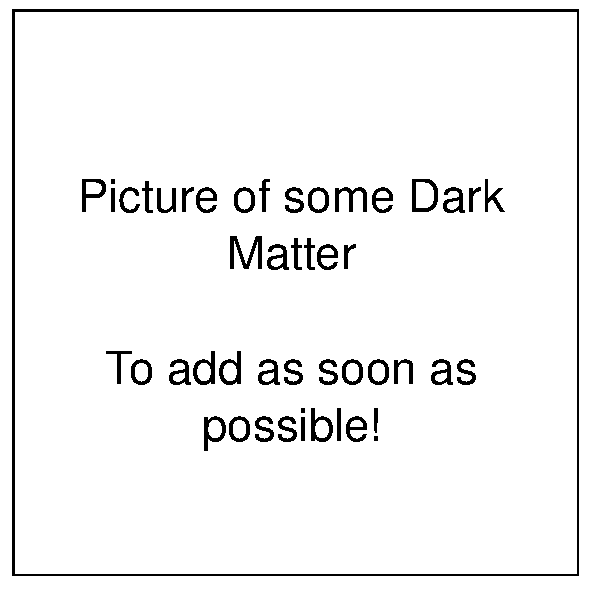
\includegraphics[width=0.3\textwidth]{Theory/figures/dark_matter_pic.pdf}
\end{figure}

The nature of dark matter (DM) is currently one of the most intriguing open questions in physics~\cite{Arbey2021}.
It's an active topic of research in astrophysics and cosmology, where it is implied as the accepted solutions for various phenomena, but is also of great interest for particle physicists, since it will inevitably go beyond the standard model.

Its existence, supported by theoretical models and experimental observations, it's widely accepted by the research community.\\
However, no direct proof has yet be found.

\subsection{Observational evidences}

There have been different evidences of the presence of DM.

\paragraph{Spiral galaxy rotational speed}

In spiral galaxies, the virial theorem dictates that the velocity of a star at distance $R$ from the center of the galaxy should follow~\cite{Belenchia2022}:
\begin{equation}
    v(R) = \sqrt{G\frac{M(R)}{R}}
\end{equation}
where $M(R)$ is the total mass contained a sphere with radius $R$.
Far from the center of the galaxy, where practically no mass is left and $M(R)$ is nearly constant, the velocity decreases as $v (R) \propto R^{-1/2}$.

However, experimental measurements of stars around spiral galaxies, performed with extremely precise Doppler shift measurements, shows a different picture.
In particular, it was observed that the velocity of stars becomes independent from the radius.
The phenomenon, visible for example in the \textit{flat rotation curves} of which \cref{fig:flat_rot_curves} are typical examples, can be explained with a halo of invisible mass of:
\begin{equation}
    M(R) = R\frac{v_0^2}{G}
\end{equation}

\begin{figure}
    \centering
    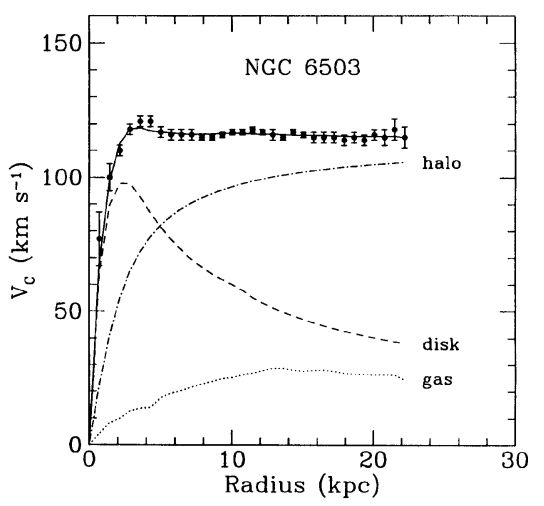
\includegraphics[width=9cm]{Theory/figures/flat_rot_curves.jpg}
    \caption[Flat rotation curves]{Galactic rotation curve for NGC 6503 showing disk and gas contribution plus the dark matter halo contribution needed to match the data. Credits to \cite{fig_rot}}
    \label{fig:flat_rot_curves}
\end{figure}

Since this mass, that seems to represent up to 80-90\% of the total mass of galaxies, appears to not interact in any way except by gravitational force, we identify it and call it as Dark Matter (DM).

\paragraph{Galaxy clusters dynamic}

A Galaxy cluster is a massive object composed of hundreds or thousands of galaxies bound together. 
In the intergalactic medium, among galaxies, it contains large quantity of gases that reach high velocities and can emit x-rays via bremsstrahlung.
This effect can be used as a way of measuring the intensity of the gravitational force and, therefore, the distribution of masses in the cluster.
The idea is that photons emitted from the center of the cluster should lose more energy than photons emitted from the edge, because of a stronger gravity.
This effect, known as \textit{gravitational redshift}, showed that a large portion of mass was not visible and distributed all around the cluster.

This method leads to results with high uncertainties, so it has been superseded by gravitational lensing techniques.

\paragraph{Gravitational lensing}

The observation of distant galaxies and galaxy clusters is usually affected by the gravitational lensing phenomenon depicted in \cref{fig:grav_lense}.
Namely, the light does not follow a straight line, being distorted by any mass between source and observer (the earth) forming the so-called \textit{Einstein circle}.

\begin{figure}
    \centering
    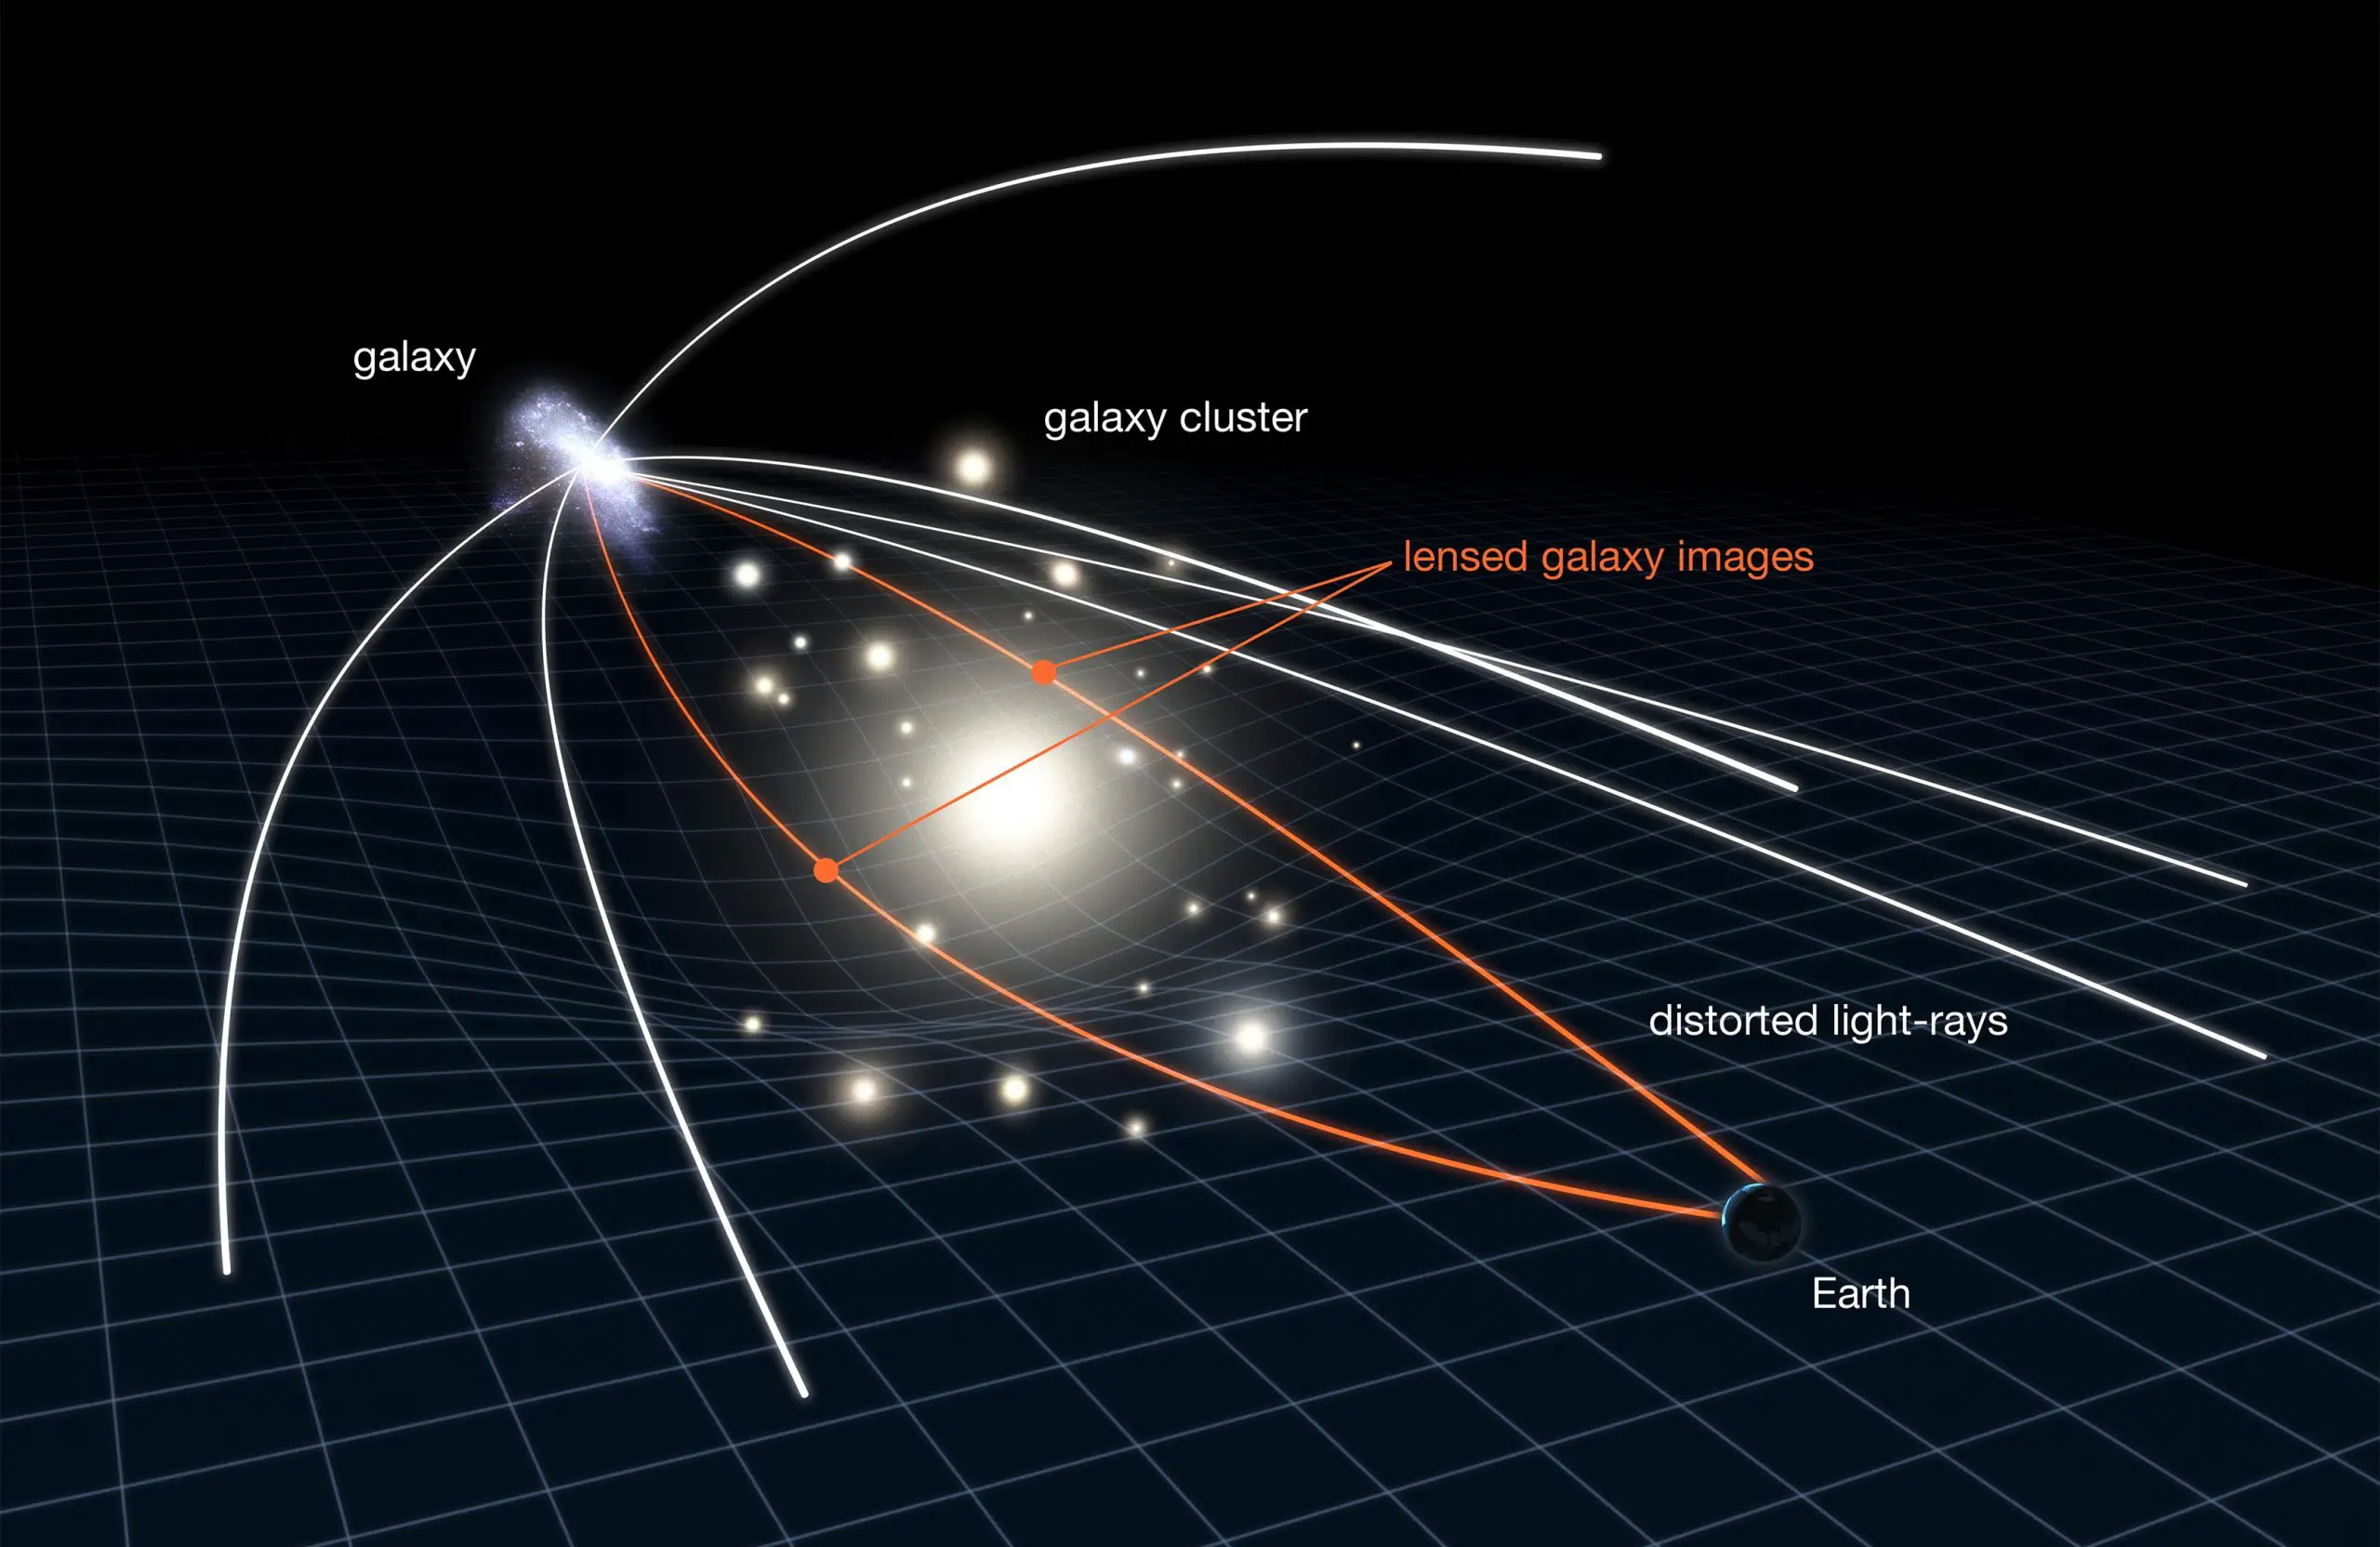
\includegraphics[width=\textwidth]{Theory/figures/gravitational_lense.png}
    \caption[Graphical depiction of gravitational lensing]{This illustration depicts the gravitational lensing phenomenon. The scale has been greatly exaggerated in this diagram. Credits to \cite{fig_lensing}}
    \label{fig:grav_lense}
\end{figure}

The radius of an Einstein circle is related to the mass which causes the light deflection following:
\begin{equation}
    \theta_E = \sqrt{\frac{4GM}{c^2}\frac{(D_S-D_L)}{D_S D_L}}
\end{equation}
with $\theta_E$ being the angular radius, $M$ the mass of the lens (in between) , $D_L$ the distance to the lens and $D_S$ the distance to the source.
This technique to weigh galaxies (and other astrophysical structures) has been used with success for many years.
Numerous studies, however, consistently reported a much larger mass measured than seen.
Again, this is explainable with presence of DM.



\paragraph{Cosmology}

The currently most widely accepted cosmological theory requires dark matter to explain the formation of structures in the early universe.

In particular, in the early universe, the energy distribution (so the mass distribution) was more or less uniform.
Two opposite processes were involved in the generation of structures: gravitational forces that were favouring structures and the expansion of the universe itself, that was "countering" structures.

In this situation, it is possible to differentiate the role of baryonic and non baryonic matter that is collisionless.
Various simulations, and in particular the Millennium Simulation~\cite{Springel2005}, were able to simulate all the early stages of the universe, with the requirement of dark matter and dark energy. 
Without DM, the current model was not able to explain nor the structures formation nor the CMB spectrum.

The current best theory, the $\Lambda$CDM (Lambda cold dark matter) shows a remarkable agreement with all the observations from disparate scales as shown in \cref{fig:convergence_dm}.

\begin{figure}
    \centering
    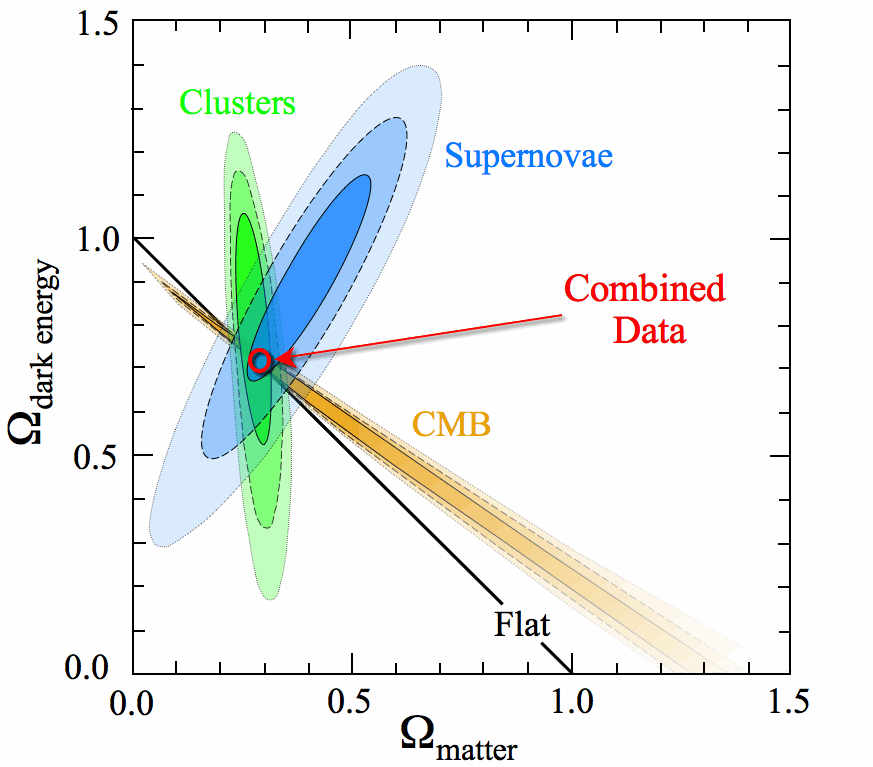
\includegraphics[width=0.6\textwidth]{Theory/figures/dark_energy_concordance.png}
    \caption[Dark Matter quantity expected from observations and theory]{Convergence of the experimental observations and of the $\Lambda$CDM model. Leading to a a percentage of $95$\% of non-baryonic energy. Credits to \cite{Einasto2009}}
    \label{fig:convergence_dm}
\end{figure}

\subsection{DM candidates}

Now that we saw the many evidences supporting the existence of dark matter, the challenge becomes to determine its nature.

We are looking for a particle (or, for what we know, a set of particles) that is stable over billions of years, collisionless, non-baryonic and interacting mostly gravitationally.

Within the Standard Model (SM), the only neutral non-baryonic particles are the neutrinos that are, however, very light particles.
This leads neutrinos to be generally relativistic, constituting an example of fast or "hot" DM.
The CMB spectrum, however, cannot be properly explained with only "hot" (relativistic) DM and rather requires the presence of a large quantity of "cold" (non relativistic) particles.
Therefore the neutrinos can eventually explain just a minimal portion of the hidden mass.
We need to find new particles, beyond SM.

Tens of candidates, of which the main ones are shown in \cref{fig:dm_candidates}, have been proposed over the years, but none has been yet successfully discovered. Indeed this is also referred to as the "dark matter candidates zoo", because of the large and never ending number of proposed new  particles.\\
Since this thesis is not directly focused on DM, we will briefly mention the two main candidates: WIMPs (weakly interacting massive particles) and axions.

\begin{figure}[ht]
    \centering
    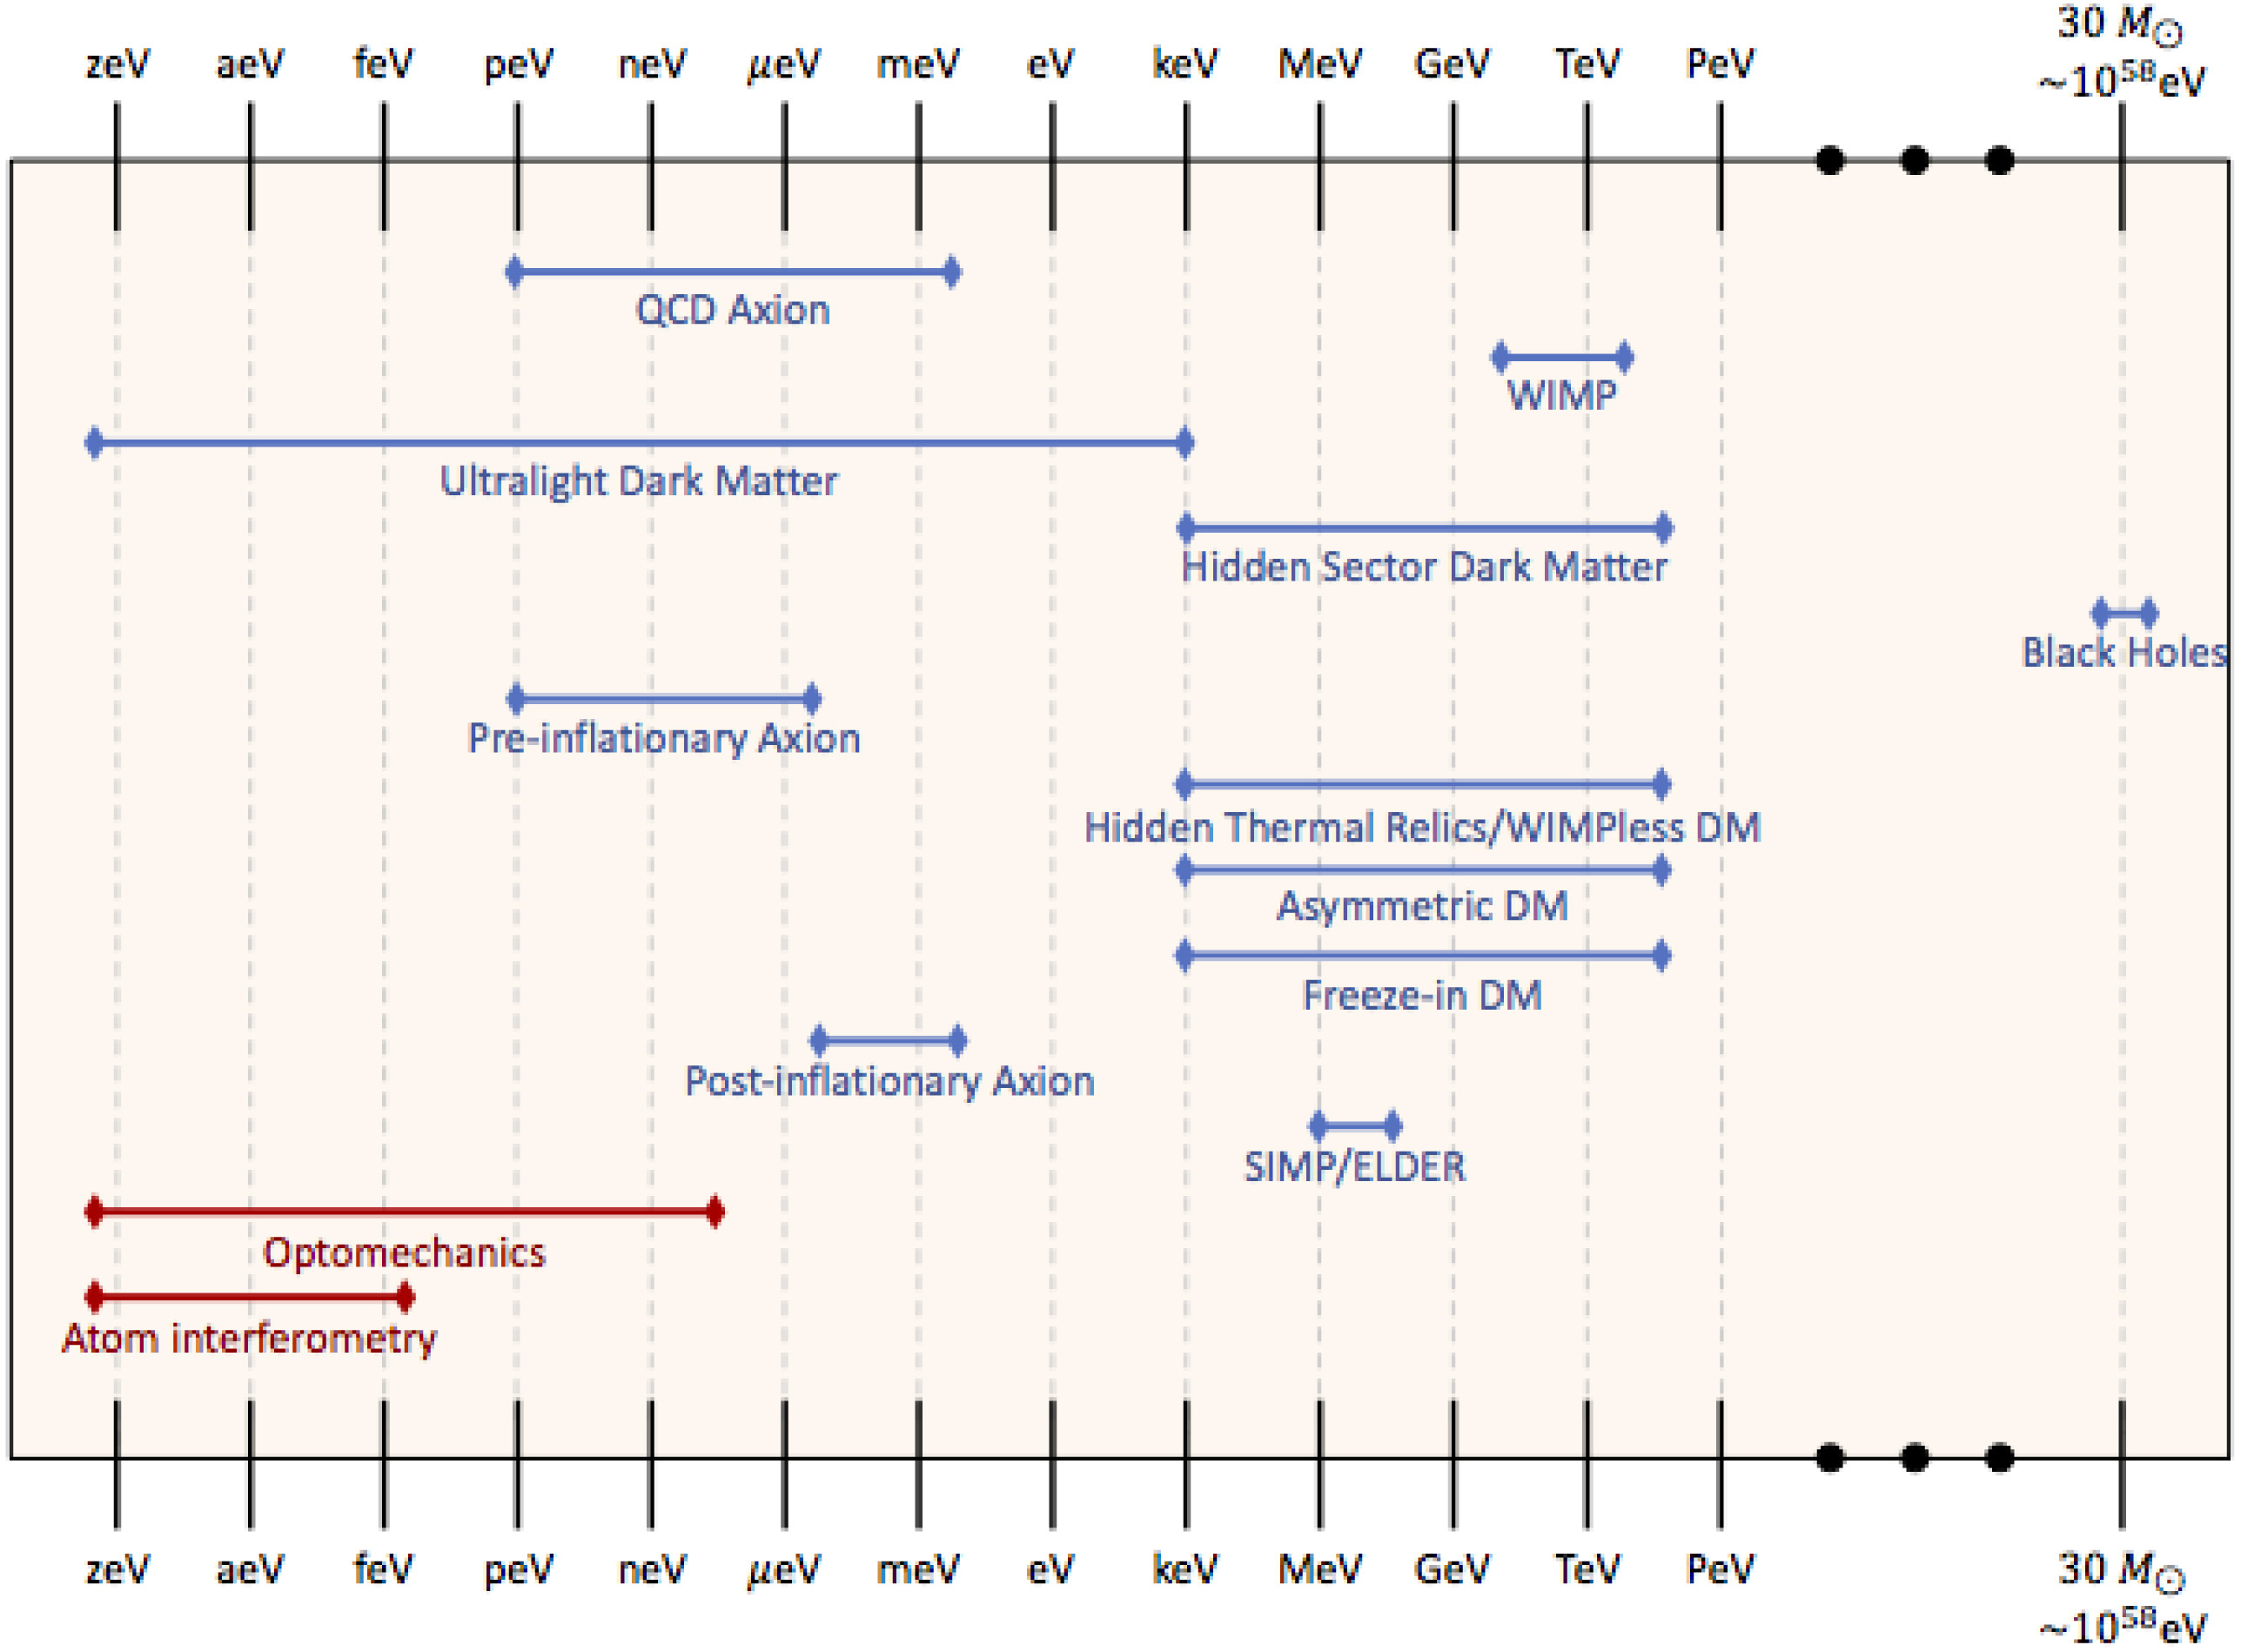
\includegraphics[width=\textwidth]{Theory/figures/candidates_dm.jpg}
    \caption[Dark Matter candidates]{DM candidates, in respect to the possible masses. Credits to \cite{Belenchia2022}}
    \label{fig:dm_candidates}
\end{figure}


\paragraph{WIMPs} were, until very recently, the most prominent DM candidate. With the name of WIMPs, various particles were described. They were supposed to have been produced thermally in the early universe (as the SM particles) with a mass of $\approx 100$ GeV. The introduction of WIMPs was often referred to as the "WIMPs miracle" since these particles are "automatically" introduced with a minimal extension of the SM to a super-symmetric theory. Moreover, WIMPs should have been detectable both indirectly, looking at annihilation products, and directly in collision experiments. No experiment\footnote{With the notable exception of the non-reproducible results of DAMA~\cite{Petriello2008}.} has ever found direct evidence and, lately, the hype for super-symmetric theories has also been decreasing, since no evidence has yet to be found ad LHC and other colliders (although it was indeed expected).

\paragraph{Dark Photons}~\cite{Caputo2021} introduce an intriguing dimension to the realm of dark matter, akin to WIMPs and axions. These hypothetical particles, often associated with hidden or "dark" forces that operate outside the framework of the Standard Model of particle physics, are captivating for their unique characteristics. Dark photons are postulated as mediators of a novel force, commonly termed the "dark force," which interacts exceptionally weakly with ordinary matter. Just as with their counterparts, dark photons may trace their origins back to the early universe, potentially emerging through mechanisms reminiscent of WIMPs.
Dark Photons still are a viable candidate, but require a large theoretical extension of the Standard Model and, being also particularly difficult to detect, are often discarded in comparison to other candidates. 

\paragraph{Axions} The original axion model is related to the strong violation of the charge conjugation (C) and parity (P) symmetries (CP-violation). The QCD Lagrangian can be written as 
\begin{equation}
    \mathcal L _{QCD} = \mathcal L _{QCD, perturbative} + \Bar{\theta} \frac{g^2}{32 \pi^2} G^a_{\mu \nu} \Bar{G}^a_{\mu \nu}
\end{equation}
where $G^a_{\mu \nu}$ is the gluon tensor, $\Bar{G}^a_{\mu \nu}$ its dual and $\Bar{\theta}$ a constant. The first term is the standard perturbative Lagrangian and the second one is an effective term coming from the topological properties of non-Abelian gauge theories and from the diagonalization of the quark mass matrix.
The problem with this term is that it violates the P and CP symmetries and measurements on the neutron electric dipole moment reveal no violation of those symmetries for the strong-force. 
A solution for this missing violation was proposed by Peccei and Quinn, in which the constant is substitute with a dynamical term coming from a new chiral global symmetry $U(1)$. This new symmetry spontaneously break and gives rise to a new scalar boson, called "axion". The symmetry also generates a new term in the Lagrangian, that removes the violation. From theory we have that:
\begin{equation}
    m \approx \frac{\Lambda^2_{QCD}}{f_a}
\end{equation}
where $m$ is the expected mass of the new particle (ranging from $\mu$eV and eV), $\Lambda_{QCD}\approx 200$ MeV and $f_a$ is a constant with the dimension of an energy, of the order of the symmetry breaking scale.

Axions are an interesting candidate for these reasons: they were not introduced for DM and solve two huge problems of modern physics. They could indeed explain the missing mass of the universe, while at the same time solving the strong CP problem.




\newpage
\section{Qubits}

A possible way of detecting dark matter, in particular axions, is through the use of superconducting qubits.

A qubit is defined, in quantum computing, as a two-state quantum-mechanical system. One of the simplest systems that can show quantum properties.

A qubit can be built with very different technologies: some examples include qubits composed of polarized photons, ions and cold atoms. 
\begin{figure}[H]
    \centering
    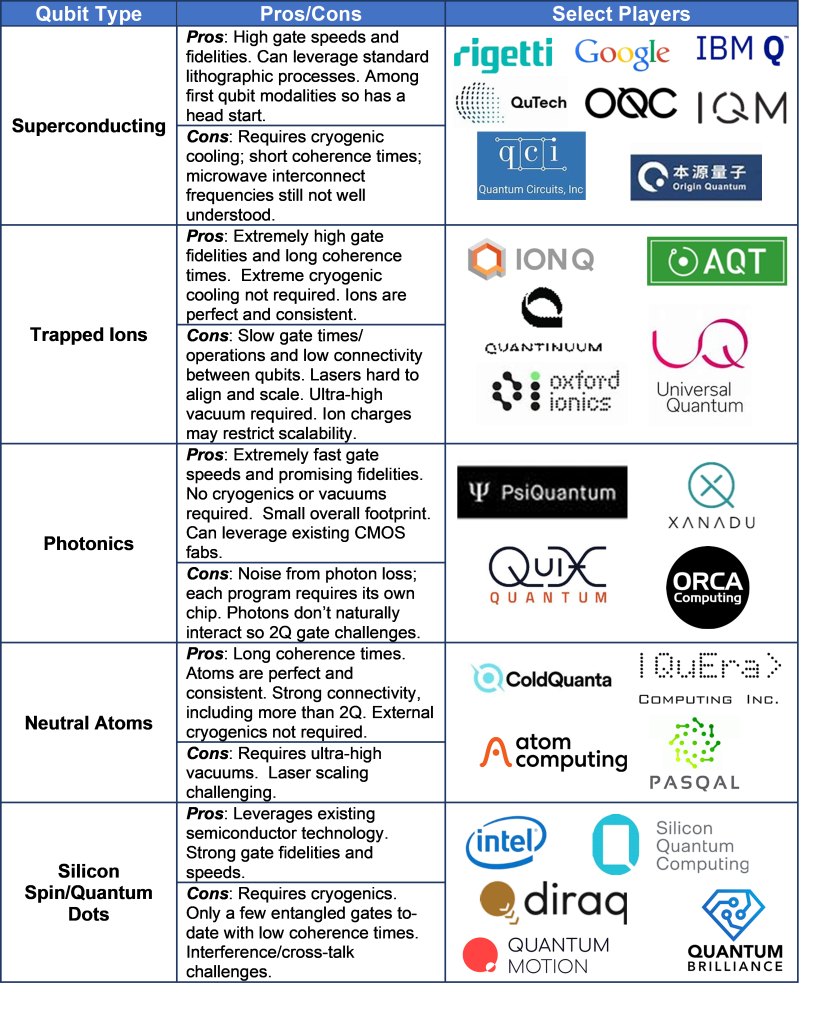
\includegraphics[width=0.8\textwidth]{Theory/figures/qubit_techs.png}
    \caption{Highlight of the main qubit technologies and companies involved in the field. Credits~\cite{quantumtech-blog}.}
    \label{fig:qubit_players}
\end{figure}
In \cref{fig:qubit_players} some of the main companies researching in quantum computing are shown, together with indication on the qubit technology used.
The preferred qubits in the last years were superconducting-based. 
In this thesis, these will be the utilized qubits.


Superconducting qubits are often called artificial atoms and the main idea behind them, is to build a circuit with the first two level very distinguishable from the others. 
So the qubit is obtained by restraining the system.

The superconducting technology has reached very good results~\cite{Arute2019}, but it is still dealing with huge problems also in the hardware and design section.

\subsection{Josephson junction}

To obverse quantum behaviour at a macroscopic level, (so at the size of circuit components), a strong degree of coherence is needed.
In superconducting qubits this is achieved exploiting the phenomenon of superconductivity that is found in some specific metals at cryogenic temperatures~\cite{Tinkham2004}.\\
At these temperatures (i.e. $T\ll T_c$ where $T_c$ is the critical temperature of the material), electrons bound together forming \textit{Cooper pairs} composed of two electrons with equal and opposite momenta~\cite{Langford2013}.
Cooper pairs have a bosonic nature, allowing them to form a condensate, where they are all described by a single quantum ground state, effectively creating a macroscopic quantum phenomenon.
To assure that the number of Cooper pairs remains stable and increase coherence times, superconducting qubits are usually operated below $50$ mK by exploiting complex cryogenics system called cryostat~\cite{Pobell2007}.

The core of a superconducting qubit is the \textit{Josephson junction}~\cite{Kockum2019}: a superconducting inductor that enables the transformation from a harmonic oscillator (standard LC circuit) to an an-harmonic oscillator, needed to separate the 0-1 states and build a qubit.\\
A Josephson junction is composed by a thin insulative gap (order of nm) between two superconductors as presented in \cref{fig:junction}.
The small thickness of the insulator enables the Cooper pairs wavefunction in the two superconductors to overlap, creating a coherent tunneling phenomenon where Cooper pairs can "jump" from one superconductor to the other without any applied voltage.
The resulting current (often referred to as \textit{supercurrent}) has a nonlinear dependence on the voltage applied over the junction, causing the anharmonicity.

\begin{figure}[ht]
    \centering
    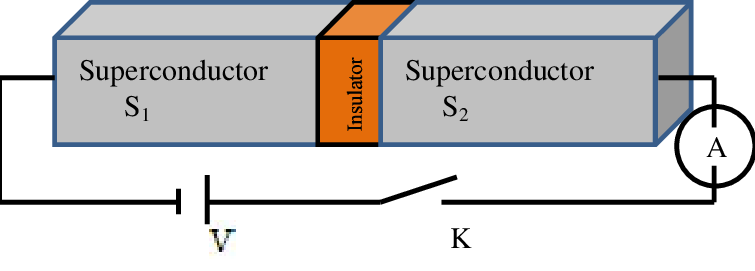
\includegraphics[width=0.6\textwidth]{Theory/figures/josephson_junction.png}
    \caption[Schematic drawing of a Josephson junction]{Schematic drawing of a Josephson junction. Credits~\cite{Vool2017}.}
    \label{fig:junction}
\end{figure}

The Hamiltonian of the Josephson junction can be found from the two equations under the name of \textit{Josephson effect}~\cite{FundamentalsAndFrontiersJosephsonEffect, Josephson1962}:
\begin{align}
    \label{eq:jos_eff_DC}
    I &= I_c \sin \phi \\
    \label{eq:jos_eff_AC}
    \pd{\phi}{t} &= \frac{2e}{\hbar}V
\end{align}
where $I$ is the supercurrent flowing through the junction, $I_c=2eE_J/\hbar$ is the critical current over which the junction starts to exhibit dissipation, $V$ is the voltage applied over the junction and $\phi$, called Josephson phase, is the phase difference between the wavefunction of the two superconductors. 
$E_J$, called Josephson energy, is the energy associated with a single Cooper pair that tunnels through the junction and can be computed as $E_J=L_J I_c^2$ with $L_J=\hbar/2eI_c$ being the inductance of the junction.

The relations expressed in \cref{eq:jos_eff_DC} and \cref{eq:jos_eff_AC} can be used to find the I-V relation:
\begin{equation}
    \pd{I}{t}=\pd{I}{\phi}\pd{\phi}{t} = I_c \frac{2e}{\hbar}V\cos\phi
\end{equation}
That gives an effective inductance term of $L(\phi)=L_J/\cos\phi$ and a inductance Hamiltonian of:
\begin{equation}
    H_L=-E_J\cos\phi
\end{equation}
The physical arrangement of the junction is extremely similar to a parallel plate capacitance and, indeed, this add to the Hamiltonian a capacitive part:
\begin{equation}
    H_C=\frac{Q^2}{2C}=\frac{(2en)^2}{2C} = \frac{4e^2n^2}{2C} = 4E_C n^2
\end{equation}
where we defined the charging energy of a single \textit{electron} as $E_C=e^2/2C$ and $n$ is the number of electron on the capacitor.

Overall, the Hamiltonian of the junction is:
\begin{equation}
    H=H_C+H_L=4E_Cn^2 - E_J \cos \phi
\end{equation}

For now, $n$ and $\phi$ where simple classical variables, now we elevate them to be quantum operators that satisfy the commutator $\left[\hat\phi,\hat n\right]=i$.
For clarity, we will use a \textit{Cooper pair box} (CPB) as system and not a standalone junction~\cite{Bladh2005}. A scheme is presented in \cref{fig:CPB}. 

\begin{figure}[ht]
    \centering
    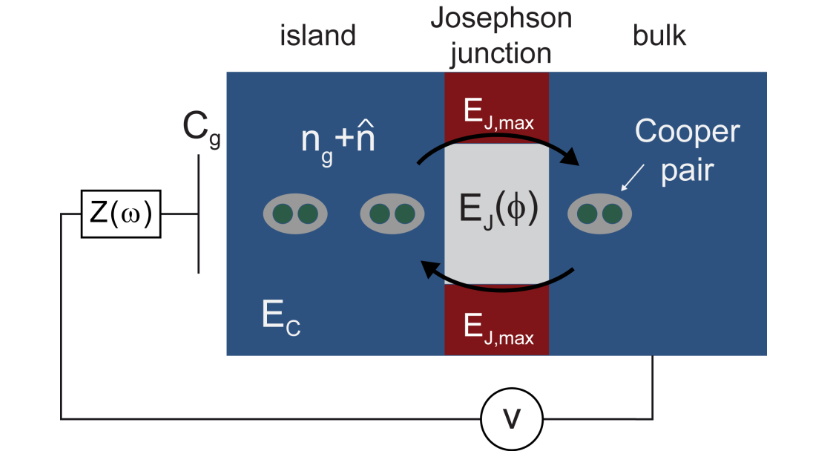
\includegraphics[width=0.6\textwidth]{Theory/figures/CPB.png}
    \caption[Scheme of a Cooper pair box]{Scheme of a Cooper pair box (CPB). Credits~\cite{CPBimage}.}
    \label{fig:CPB}
\end{figure}

The Hamiltonian is almost identical, but we add a $n_g$ term that is the offset charge induced by a voltage source:
\begin{equation}
    H = 4E_C (n-n_g)^2 - E_J \cos\phi \rightarrow  \hat H = 4E_C (\hat n-n_g)^2 - E_J \cos{\hat \phi}
\end{equation}

For a typical CPB we have $E_J/E_C < 1$ so we can express the Hamiltonian in term of \textit{charge states} $\ket N$, namely the eigenstates of $\hat n$ (note that $\left[ \hat H, \hat n \right]=0$).
Note also that with $N$ we indicate the difference of Cooper pairs between the two islands and \textit{not} the total number of Cooper pairs that would be impractical.\\
We can write~\cite{Vool2017}:
\begin{align}
    4E_C(\hat n - n_g)^2 &= 4E_C \sum_N (N-n_g)^2 \ket N \bra N \\
    -E_J \cos{ \hat \phi} &= \frac{E_J}{2}\sum_N (\ket N \bra{N + 1} + \ket{N+1} \bra N)
\end{align}
Note that $\ket N \bra N$ is essentially the number operator for the Cooper pairs, while $\ket N \bra{N+1}$ represents the coherent transfer of a single Cooper pair from island to the reservoir (and the other combination the opposite transfer).

\subsubsection{Flux-tunable Josephson junction}\label{sec:flux_tunable_junction}

A single Josephson junction can be used to build a qubit, but its resonance frequency will be fixed by a relation with $E_J$.
For various reasons, and in particular to achieve two-qubits interactions, it is important to have the capability of "freely" controlling the resonance frequency.

To achieve this tunability, we substitute the Josephson junction with a \textit{superconducting quantum interference device} (SQUID), namely two junctions connected in a loop.
The SQUID, depicted in \cref{fig:squid}, roughly behaves like a single junction, but its Josephson energy is dependent on an external magnetic flux that may run through the loop, thus giving us tunability.

\begin{figure}[ht]
    \centering
    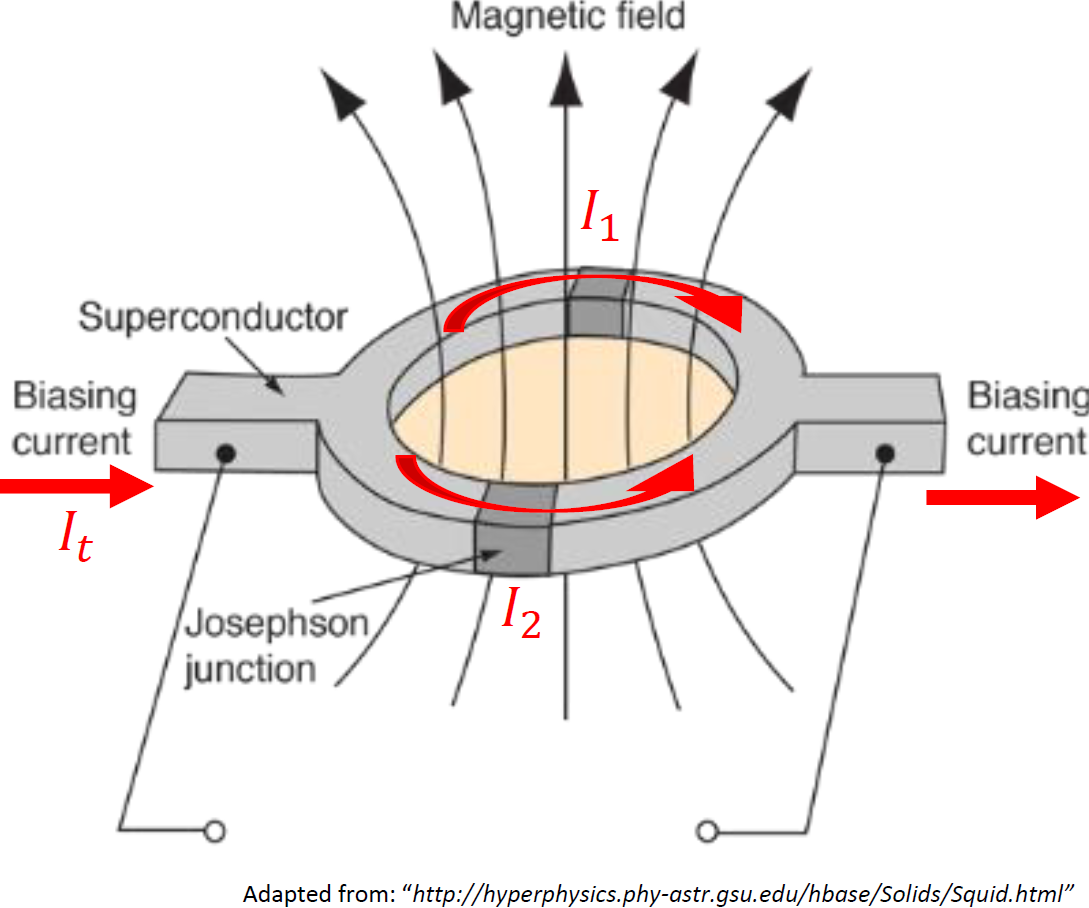
\includegraphics[width=0.5\textwidth]{Theory/figures/squid.png}
    \caption{Schematic layout of a SQUID.}
    \label{fig:squid}
\end{figure}

Let us return to the inductance Hamiltonian (non as an operator), that for a SQUID is:
\begin{equation}
    H_L=-E_J \cos{\phi_1}-E_J \cos{\phi_2}
\end{equation}
where we are assuming that the two junctions are identical (so $E_{J1}=E_{J2}+E_J$).
This simplifies the calculations here, but note that in reality the two energies are purposefully made different to limit the tuning range of the SQUID~\cite{Koch2007}.\\
Between the two phases there is a strict relation:
\begin{equation}
    \phi_1 - \phi_2 = 2\pi l + 2\pi \Phi/\Phi_0
\end{equation}
where we considered two phenomena: the difference in phase, without external flux, must be a multiple of $2\pi$ ($l$ here is an integer) so that the wavefunction is single-valued; and the addition of an external flux $\Phi$ changes the overall phase by a factor dependent on the ration between $\Phi$ and $\Phi_0=h/2e$, the superconducting flux quantum.

So we can now write:
\begin{equation}\label{eq:hl_flux_tunable}
    H_L = -2E_J \cos \left( \frac{\phi_1 - \phi_2}{2} \right) \cos \left( \frac{\phi_1  \phi_2}{2} \right) = -E_{J\Phi} \cos \phi
\end{equation}
where we defined $\phi=(\phi_1 + \phi_2)/2$ and $E_{J\Phi} = 2E_J\cos (\pi \Phi / \Phi_0)$.

So we re-obtain the same exact Hamiltonian form than the simple Josephson junction, but with a tunable $E_J$.

\subsection{Transmon qubits}

A Cooper pair box can already work as a qubit, but the its property are not ideal.
In general, we use a variation called \textit{transmon}.\\
A transmon qubit is a CPB shunted by a capacitor that is large in respect to the capacity of the junction.
The result is the characteristic ratio $E_j/E_C \gg 1$ (CPB usually have $E_J/E_C < 1$).

The physical implementation of a transmon is usually very different from a CPB (in particular for XMONs, the main transmon architecture), but the Hamiltonian is always of the same form.
The eigenvalues, however, are extremely dependent on the $E_J/E_C$ ratio, as visible in \cref{fig:levels-ratio}.
\begin{figure}[ht]
    \centering
    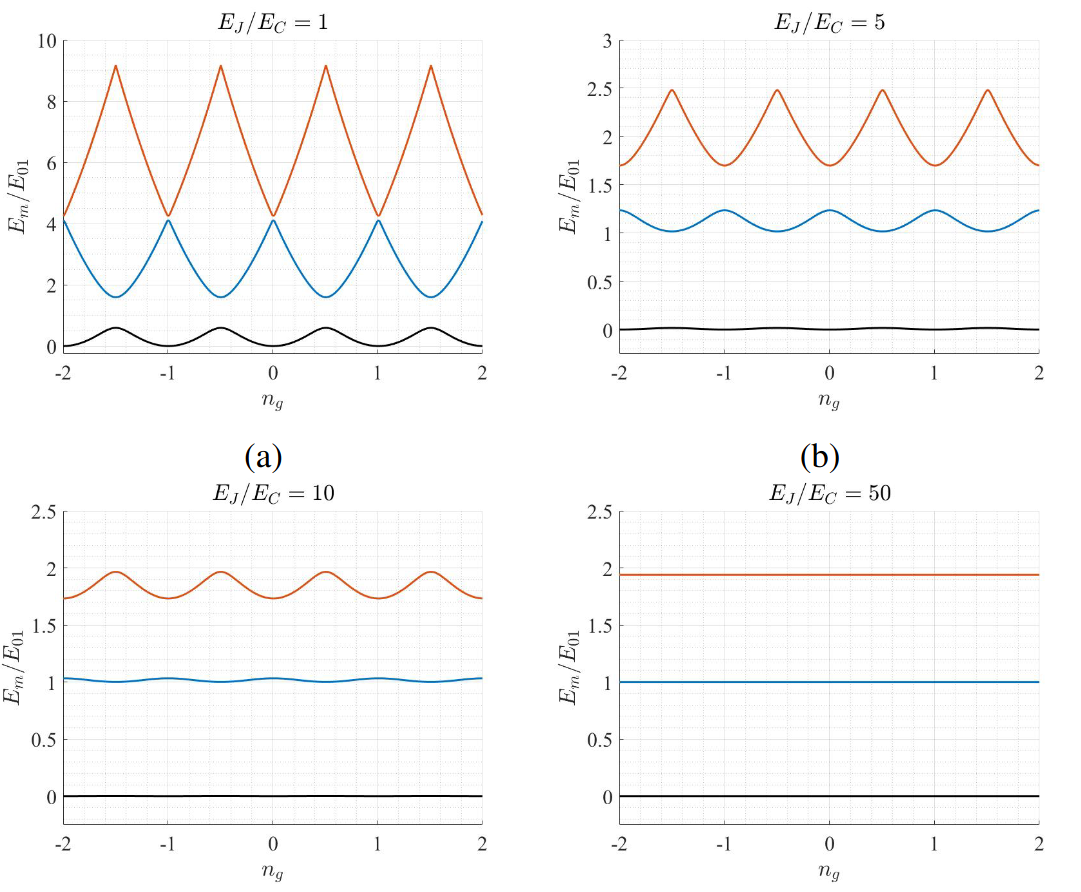
\includegraphics[width=\textwidth]{Theory/figures/levels_ratio.png}
    \caption[Comparison of qubit Hamiltonian eigenvalues for different ratios of $E_J/E_C$.]{Comparison of the Hamiltonian eigenvalues for different ratios of $E_J/E_C$. Credits \cite{Roth2021}.}
    \label{fig:levels-ratio}
\end{figure}
In the transmon limit the energy levels are extremely flat in respect to $n_g$, so much more stable, but also more harmonic.
Since the sensitivity from charge noise decreases faster than the anharmonicity, then we achieve a practical insensitivity from charge noise, while still having enough anharmonicity to consider the system a qubit (typically we have transition of $\approx 10$ GHz and anharmonicities of $\approx 200$ MHz).

The Hamiltonian of this system, derivable from classical circuits Hamiltonians, can be written as:
\begin{equation}\label{eq:hamiltonian_transmon}
    \hat H = 4 E_c (\hat n - n_g ) ^ 2 - E_J \cos \hat\phi
\end{equation}

\subsubsection{Flux tunable qubits}\label{sec:flux_tunable_qubits}

The introduction of a SQUID instead of a single junction leads, as we have seen in \cref{sec:flux_tunable_junction}, to flux tunability of $E_J$. For identical junctions in the SQUID we have:
\begin{equation}
    E_J = E_{j,max} \left|  \cos (\pi \Phi / \Phi_0)  \right|
\end{equation}
where the external magnetic flux is $\Phi$.

This flux dependency will be exploited in two-qubit gates applications, but also has some major drawbacks.

The idea is that, changing $E_J$, the first effect is to change the transition frequency 0-1 of the qubit. This follows the relation:
\begin{equation}
    f (\Phi) \approx \frac{1}{h} \left ( \sqrt{8 E_J E_C \left| \cos \left ( \pi \frac{\Phi}{\Phi_0} \right) \right|} - E_C \right)
\end{equation}

This gets translated into saying that the frequency is tunable by applying external flux, but also that spurious magnetic currents will affect the qubit.

It is currently not possible to completely remove magnetic fluxes "trapped" in a cryostat and the problem becomes worse when you know that, for every warm up the trapped flux changes and the qubit needs to be re-calibrated.

However, flux-tunable qubits offers a straightforward way of implementing two-qubit interactions, "moving" one qubit frequency to the same value of a neighbor qubit, causing hybridization of states and creation of polarons.

Note that the flux-tunable technology is not the only one for implementing two-qubit interactions. For example, IBM, one of the most important player in the superconducting qubit development, never used flux tunable qubits for their backend and even Nakamura's lab (one of the most prominent labs in the word) is moving away from them, because of the problems related to flux-noise.

In any case, it is possible to minimize the sensitivity of the transition frequency, using a special bias value. The charge-degeneracy point $n_g = 1/2$, that identifies the so-called \textit{sweetspot}.
The idea is to move the qubit to its maximum frequency, where we have that higher \textit{and} lower biases both lead to a decrease.

Since the charge dispersion has no slope there, linear noise contributions cannot change the qubit transition frequency.
With this procedure, the unfavorable sensitivity of CPBs to charge noise can be improved significantly, potentially raising T2 times from the nanosecond to the microsecond range.
Unfortunately, the long-time stability of CPBs at the sweet spot still suffers from large fluctuations which drive the system out of the sweet spot and necessitate a resetting of the gate voltage.




\section{Transmon interactions}

An isolated transmon offers no mean of control and readout, so it is completely useless.
We have to add components for readout, drive (control of the qubit state) and flux (control of the qubit frequency).

For a single qubit, we can expect a scheme like the one represented in \cref{fig:scheme-basic_interaction}.

\begin{figure}[ht]
    \centering
    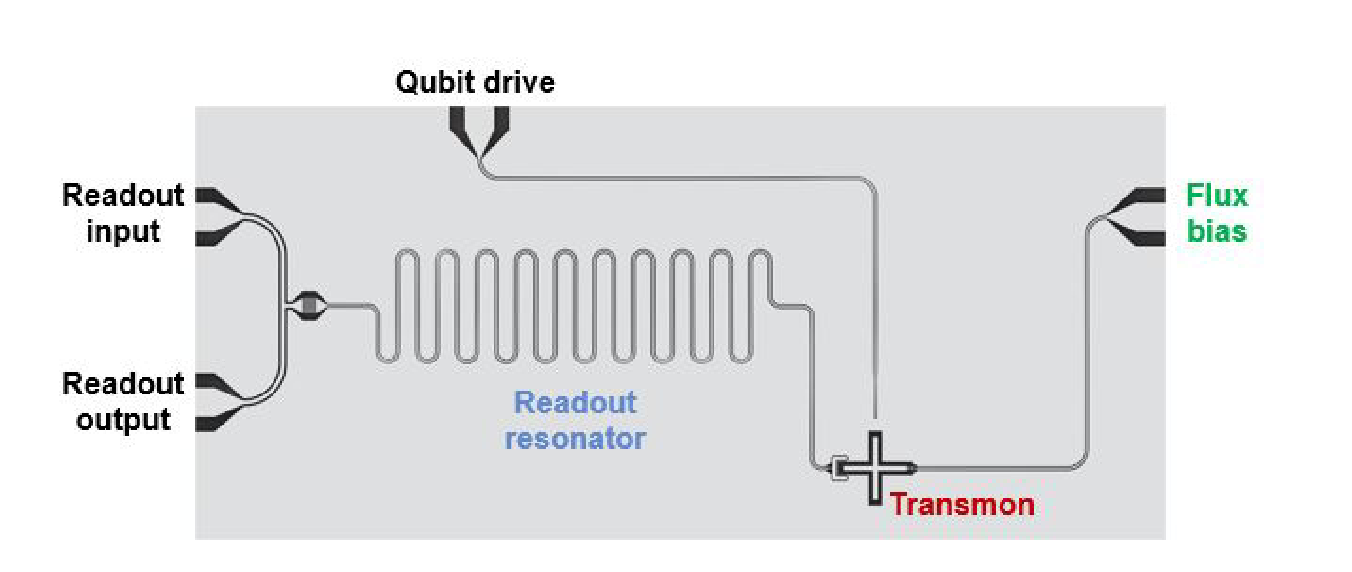
\includegraphics[width=0.8\textwidth]{Theory/figures/scheme_basic_interactions.png}
    \caption{Basic scheme for the complete control of a single flux-tunable transmon.}
    \label{fig:scheme-basic_interaction}
\end{figure}

In \cref{fig:scheme-basic_interaction} we can see all the standard lines present in a single qubit system:

\begin{description}
    \item[Readout input:] a line where a signal can be send to probe a resonator that is coupled to the qubit and, because of this, dependent on its state;
    \item[Readout output (feedback):] a line where the sent readout signal gets acquired, after the resonator interaction. This signal can be the input {\it reflected signal} (as in the scheme presented) or, in some configurations, the {\it transmitted signal}
    \item[Drive:] a line coupled to the qubit, that we can use to change the qubit state itself;
    \item[Flux:] a line that contains an inductor, so that a DC current passing through it can generate a magnetic field to change the qubit frequency.
\end{description}

An illustration, in circuit form, of the system is presented in \cref{fig:circuit-basic_interaction}.

\begin{figure}[ht]
    \centering
    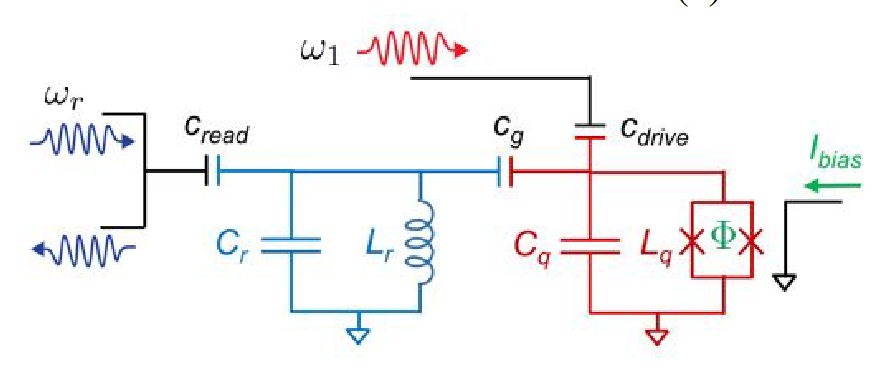
\includegraphics[width=0.8\textwidth]{Theory/figures/scheme_basic_interactions2.png}
    \caption{Basic circuit scheme for the complete control of a single flux-tunable transmon.}
    \label{fig:circuit-basic_interaction}
\end{figure}

To study the system we can start writing the Hamiltonian of the resonator-qubit system.
We can express the diagonalized qubit Hamiltonian, non limited to the first two states, as:
\begin{equation}
    \hat H_T = \sum_j \hbar \omega_j \ket j \bra j
\end{equation}
where $\omega_j$ is the eigenvalue associated with the $\ket j$ eigenstate.

The resonator Hamiltonian can be written in the standard harmonic oscillator form:
\begin{equation}
    \hat H_R = \hbar \omega_r \hat a^\dagger \hat a
\end{equation}

The total Hamiltonian of the system will add one more term:
\begin{equation}
    \hat H = \hat H_T + \hat H_R + \hat H_I
\end{equation}

The interaction term can be written as:
\begin{equation}
    \hat H_I = 2e \frac{C_g}{C_g+C_q}\hat V_r \hat n= 2e \frac{C_g}{C_g+C_q}V_{rms} (\hat a + \hat a ^ \dagger) \hat n
\end{equation}
where $\hat V_r$ is the resonator voltage operator and $V_{rms}=\sqrt{\hbar \omega/2C_r}$.\\
If we write the qubit charge operator in terms of the transmon eigenstates, define the coupling $g_j=2e\frac{C_g}{C_g+C_q} V_{rms} \bra{j-1} \hat n \ket{j}$ and simplify the equation considering only the relevant terms:
\begin{equation}\label{eq:jaynes-cummings-generalized}
    \hat H = \sum_j \hbar \omega_j \ket j \bra j + \hbar \omega_r \hat a^\dagger \hat a + \sum_j g_j (\ket{j-1} \bra{j}\hat a^\dagger  + \ket j \bra{j-1} \hat a)
\end{equation}
this equation is usually called \textit{Jaynes-Cummings Hamiltonian}.

To understand the simplification we can write the generalized Jaynes-Cumming Hamiltonian as:
\begin{equation}
    \hat H = \omega_r(\hat a ^ \dagger \hat a) - \frac{1}{2}\omega_1\sigma_z - g(\hat a ^ \dagger + \hat a)(\sigma_-+\sigma_+)
\end{equation}
where $\sigma_z$  is the Z Pauli matrix and the $\sigma_\pm$ are the transmon ladder operators.\\
This representation does not add anything to the previous one, but it could maybe be a bit more easy to understand when we focus on the interacting Hamiltonian:
\begin{equation}
    \hat H_{I} = \hat a ^ \dagger \sigma_- + \hat a \sigma_+ + \hat a ^ \dagger \sigma_+ + \hat a \sigma_-
\end{equation}
The first term describes a qubit decay while creating a new photon in the resonator and so on.\\
Now it's easy to identify that, of those 4 terms, only 2 conserve the energy and are much less likely to occur.
Actually, using the \textit{Rotating Wave Approximation} (RWA), we can remove these terms, reaching again the form of \cref{eq:jaynes-cummings-generalized}.

In the dispersive regime ($\Delta = \abs{\omega_j - \omega_r}\gg g_j$) we can define the \textit{dispersive shift} $\chi = g_1^2/\abs{\omega_1-\omega_r}$ and, considering only $\ket 0$ and $\ket 1$ as the first two transmon states, write:
\begin{equation}
    \hat H = \hbar (\omega_r - \chi \ket 1 \bra 1 + \chi \ket 0 \bra 0 ) \hat a ^ \dagger \hat a + \frac{\hbar}{2}(\omega_1 + \chi) (\ket 0 \bra 0 - \ket 1 \bra 1)
\end{equation}
or better:
\begin{equation}\label{eq:readout_equation}
    \hat H = (\omega_r - \chi \sigma_z) \hat a ^\dagger \hat a - \frac{1}{2}\omega_q\sigma_z
\end{equation}
where $sigma_z$ is the Pauli matrix and $\omega_q =\omega_1$.

This is the relation exploited in the standard transmon readout scheme.



\subsection{Control and readout}

\subsubsection{Driving a qubit}

Ignoring the resonator, we can consider the dynamic Hamiltonian of a driven qubit with:
\begin{equation}
    H_{\text{drive}} = -\frac{1}{2}\omega_q \sigma_z - E(t) \cdot \hat d 
\end{equation}
where we are considering a classical coherent signal with dipole interaction: $E(t)=E\cos(\omega_d t)$.
If the dipoles are aligned we can simplify  the Hamiltonian as:
\begin{equation}\label{eq:drive_hamiltonian}
    H_{\text{drive}} = -\frac{1}{2}\omega_q \sigma_z - A\cos(\omega_d t) \sigma_x
\end{equation}

We can describe the interacting qubit dynamic considering a state:
\begin{equation}
    \ket{\psi(t)} = C_0 (t) e^{+i\frac{\omega_q}{2}}\ket 0 + C_1 (t) e^{-i\frac{\omega_q}{2}}\ket 1
\end{equation}
Solving the Schrodinger equation we obtain:
\begin{align}
    C_0(t) &= \frac{e^{-i\frac{\Delta_d}{2}t}}{\Omega_R}\left(  \Omega_R \cos\left( \frac{\Omega_R}{2}t \right) + i \Delta_d \sin \left( \frac{\Omega_R}{2}t \right) \right)\\
    C_1(t) &= i \frac{Ae^{i\frac{\Delta_d}{2}t}}{\Omega_R}\sin \left( \frac{\Omega_R}{2}t \right)
\end{align}
where we defined $\Delta_d = \omega_q - \omega_d$, $A=Ed$ and $\Omega_R=\sqrt{A^2+\Delta^2_d}$.

These equations describe the dynamic of a driven qubit.
We can extract the solution in terms of probabilities:
\begin{equation}\label{eq:probability_1}
    P_1(t) = \abs{C_1(t)}^2= \frac{A^2}{A^2 + \Delta_d^2}\sin^2\left( \frac{\sqrt{A^2+\Delta_d^2}t}{2}t\right)
\end{equation}

\subsubsection{Measurements}

To measure the state of a qubit, we will never probe it directly but rather use \cref{eq:readout_equation} to our advantage.

The idea is that the effective resonance frequency of the resonator will be dependent on the state of the qubit as: $\omega = \omega_r - \chi \sigma_z$. 
So it will be sufficient to measure this frequency to infer the qubit state.

Note that the resonance frequency corresponds to the excitation energy.

Considering the resonator at the ground state, we can identify two states: $0(G)$, corresponding to the qubit in state $\ket 0$, and $0(E)$ corresponding to the qubit in $\ket 1$. To these states, different transition energies (or frequency) will be available so we can write, defining $\gamma$ as a photon with the transition energy tuned to the excitation of the state in the underscript:
\begin{align*}
    \gamma_{0(G)} &+ 0(G) \rightarrow \ket 1(G) \\
    \gamma_{0(G)} &+ 0(E) \rightarrow \gamma_{0(G)} + 0(E) 
\end{align*}

this difference is explained considering that, in the second case, the sent photon does not have the energy tuned to the transition.

Consider first a circuit with a planar resonator. A planar resonator is a type of resonant structure designed on a single plane, typically on the surface of a printed circuit board (PCB) or a similar substrate.
The readout line, often called transmission line, will be coupled to the resonator just by proximity.
This means that, if we send a certain number of photons through the line and they are tuned to the transition frequency, they will get absorbed by the resonator that will get excited. We will therefore have "missing photons" at the end of the readout line.

The situation is sightly different in the case of a 3D resonator, in which the readout line passes within. 3D resonators are resonant structures that extend into three dimensions, and they are not confined to a single plane. Usually, in quantum computing, the typical structure is a cavity resonator.
Indeed , the phenomenon appears here in the opposite way, with an increase in the photon number for on resonance energies. This can be explained with the classic constructing interference effect seen in all kind of standing waves, as they are the ones in the 3D resonator.

So this is the very simple idea behind superconducting qubit measurements.
But what happens in case of superposition states?

From the principles of quantum mechanics, we will have the wave-function collapsing in the measured state. This should not come as a surprise, but what it's interesting to note is the non-destructiveness of this protocol.
The idea is that two consecutive measurements, should lead to the same exact result, because the measurement should not disturb the state of the qubit (note that the wavefunction collapse is not considered a disturb here).
This property is desired and expected in ideal conditions, and it is also required in numerous error correction schemes however, in real hardware, it is often not completly achievable.





%
\section{Signals}

\chapter{Experimental setup and software}
\section{Experimental setup}

In this section I will schematically present the experimental setup used for this thesis.
Note however that, being this an experimental work, the setup changed various times and it is difficult to give a complete description of it, for all the states it had.

The schematics presented here correspond to the final setup.

\subsection{Cryostat}

Since the qubits that we are considering are transmons, they work exploiting the superconductivity phenomenon.
To reach the superconductivity regime, we need a device capable of refrigerating it to the mK region.
The device employed for this task is called cryostat.

In this thesis I used both the SD and XLD cryostats manufactured by Bluefors, but the majority of the data presented here was acquired with qubits in the XLD so I will focus on the description of those last setups.

The technique used by cryostats to achieve these temperatures is the dilution refrigeration~\cite{McClintock2003, Craig2004}: a process that exploit a mixture of $^4\mathrm{He}$ and $^3\mathrm{He}$ to reach temperatures below the minimal one achievable through pressure process.
The two isotopes are quite different: the former is a boson with spin $0$ that can be found in natural gas reservoirs, while the latter is a fermion (spin $1/2$) and is the byproduct of tritium fabrication in nuclear reactors.

$\mathrm{^3He}$ can be diluted in $\mathrm{^4He}$ at any concentration, but when the mixture is cooled below $\sim 0.85$ K (note that pure liquid $\mathrm{^3He}$ can be cooled to a minimum of $0.3$ K) it undergoes a spontaneous phase separation.

Two phases now coexist: a concentrated phase composed essentially only of $\mathrm{^3He}$ and a diluted phase that, on the contrary, is mostly composed of $\mathrm{^4He}$.

\begin{figure}[ht]
    \centering
    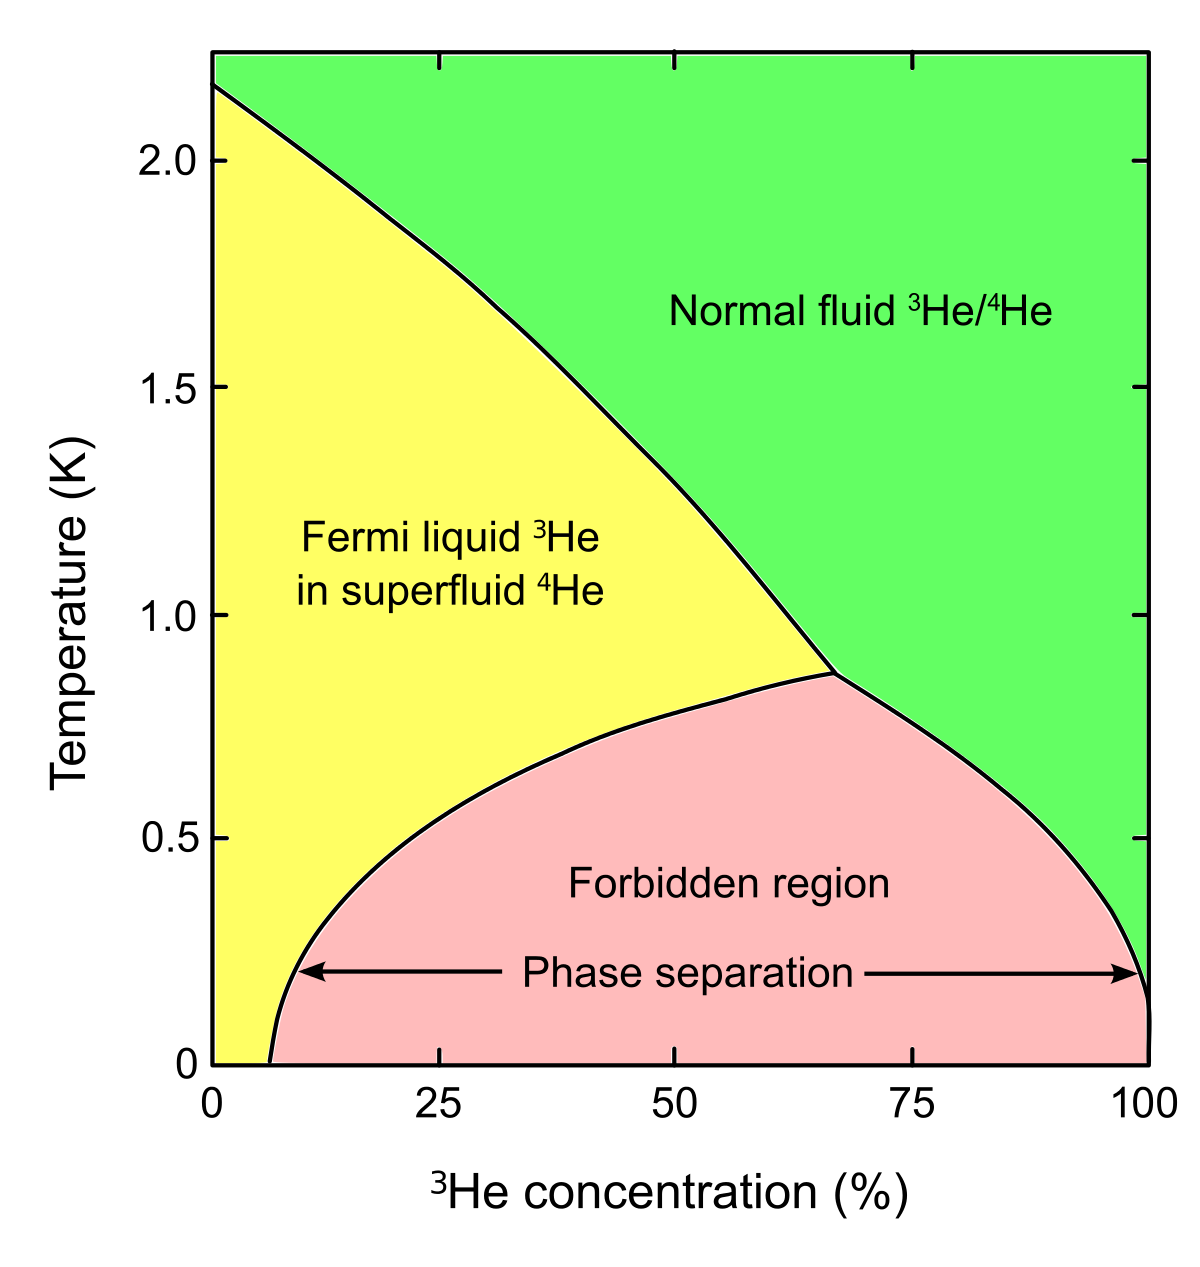
\includegraphics[width=0.6\textwidth]{Setup-software/figures/Helium_phase_diagram.svg.png}
    \caption{Phase diagram for $\mathrm{He}$ as a function of $\mathrm{^3He}$ concentration.}
    \label{fig:cryostat:heliumphasediagram}
\end{figure}

The graph in \cref{fig:cryostat:heliumphasediagram} shows equilibrium concentrations: intersections of the phase separation line and a horizontal isotherm line correspond to the concentrations of the two different phases (if below the $0.85$ mK threshold).

In the coldest part of the cryostat, the mixing chamber, $\mathrm{^3He}$ atoms cross the interface between the concentrated and the diluted phase.
This transition is endothermic and removes heat from the mixing chamber.
When $\mathrm{^3He}$ dissolves in $\mathrm{^4He}$ at such low temperatures, it undergoes a process similar to evaporation in a vacuum and produces vapor.
The diluted phase is connected to another chamber called still (short for distilling pot) that is held by a heater at $\sim0.7$ K and continuously pumped to remove the vapor which is mainly composed of $\mathrm{^3He}$ because of its greater vapor pressure.
The depletion of $\mathrm{^3He}$ within the still produces an osmotic pressure that drives more $\mathrm{^3He}$ to the still from the mixing chamber where phase transition can continue to happen.
$\mathrm{^3He}$ pumped from the still is reintroduced to the mixing chamber through a flow impedance that enables the helium to condense and that cools it down via heat exchangers that work making use of the cold $\mathrm{^3He}$ that is flowing upwards toward the still. This process is schematized in \cref{fig:cryostat:heliumdilutionrefrigerator}.

In \cref{fig:xldcryostat} some picture of the XLD are present.
Without any thermal load can reach $8$ mK, while with minimal thermal load (the qubits mounted but not probed) is stable at $9$ mK.

\begin{figure}[H]
    \centering
    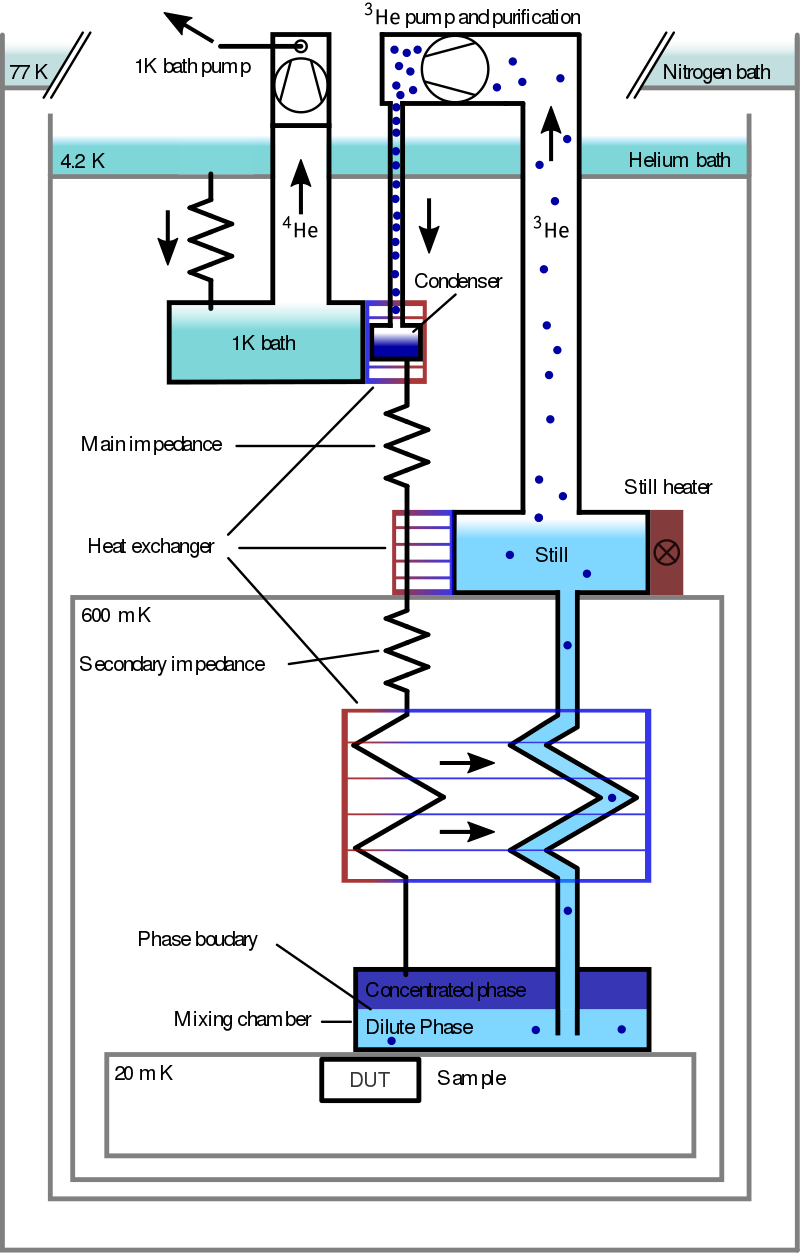
\includegraphics[width=0.6\textwidth]{Setup-software/figures/dilution_refrigerator.png}
    \caption{Outline of the dilution process.}
    \label{fig:cryostat:heliumdilutionrefrigerator}
\end{figure}


\begin{figure}[ht]
    \centering
    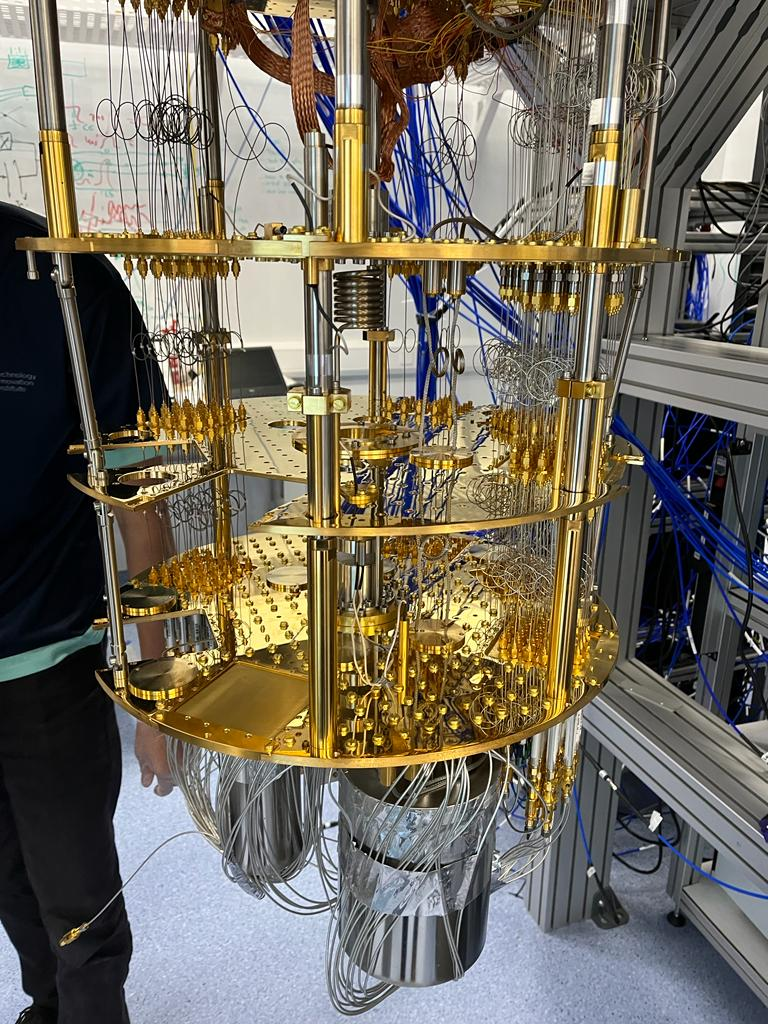
\includegraphics[width=0.55\textwidth]{Setup-software/figures/XLD.jpeg}
    \caption{Bluefors XLD.}
    \label{fig:xldcryostat}
\end{figure}

\subsection{FPGA \& RFSoC}

A Field-Programmable Gate Array (FPGA) is an electronic board that supports complete firmware configuration \textit{after} manufacturing as well as partial re-configurations while executing a specific program.\\
While integrated circuits serve a specific purpose and cannot be re-configured after fabrication, FPGAs can contain arrays of programmable logic blocks that can serve simple logic purposes (as Boolean operations) or complex functions, depending on the loaded firmware.
Since they are completely re-configurable and since they can improve the performance of standard CPU (with task-specific firmwares) without the large energy conception required by GPUs, FPGAs are rapidly becoming of widespread use.
Moreover, since the same FPGA can serve different purposes in extremely different fields, it is usually a cheap alternative to standard systems.\\
The drawback of all of this is in the overhead that programming a FPGA introduces.
To compile a FPGA firmware one first has to define the logic to use via Hardware Description Languages (HDL) then design the connections internal to the FPGA logic and conduct precise tests on the produced firmware.

The type of FPGAs used in my thesis are RFSoC, namely Radio Frequency System on Chip: their main characteristic is the capability of synthesizing directly frequency up to $\approx 10$ GHz, as well as the capability of acquiring extremely high frequency by exploiting the downsampling technique. 
All of this combined in the same board, along with a standard CPU, RAM and memory: enabling the creation of a full on-board system.\\
In this section I will provide some explanation on the techniques used for high-frequency synthesis and high frequency acquisition. 
Also, some details on the FPGAs used will be provided.

\subsubsection{Direct Digital Synthesis (DDS)}
The technique used for direct microwave synthesis is called \textit{Direct Digital Synthesis} (DDS) and it enables to use the DACs as arbitrary waveform generators for high frequencies~\cite{DDS}.

In general, a DDS system consist in a precision reference clock (often a crystal clock), an address counter, a programmable read-only memory (PROM) and a DAC (see \cref{fig:simple_DDS} for reference).\\
In the PROM, a complete cycle of a periodic function is stored and the address counter steps through it, accessing sequentially  all the PROMS's memory locations (so the PROM is working a lookup table).
The DAC then converts the input from the PROM, to analog outputs.

Note also that the PROM can be composed of two different lookup tables, for complex I-Q signals, often referred to "in-phase and quadrature signals," are a pair of time-varying signals used in signal processing and communications. They represent:
\begin{description}
    \item[In-Phase (I) Component] The "I" component represents the signal's amplitude or phase information. It corresponds to the real part of the complex signal.
    \item[Quadrature (Q) Component] The "Q" component is also a real part of the complex signal but is phase-shifted by 90 degrees relative to the "I" component. The "Q" component carries information orthogonal to that of the "I" component.
\end{description}


\begin{figure}[ht]
    \centering
    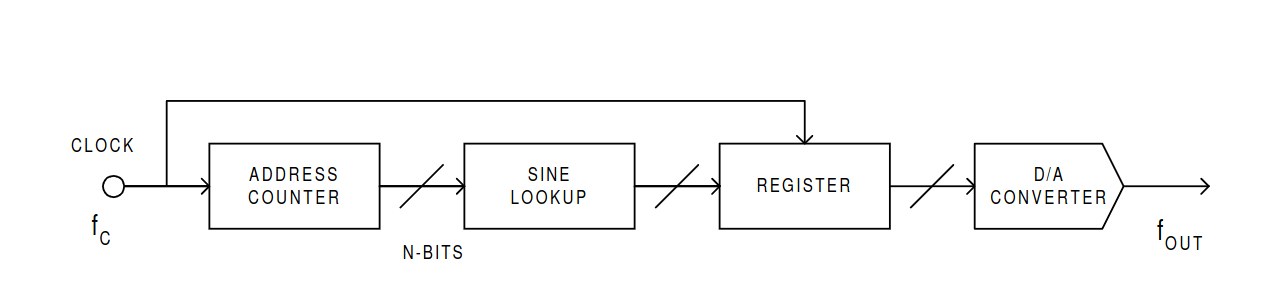
\includegraphics[width=\textwidth]{Setup-software/figures/simple_DDS.png}
    \caption{A simple Direct-Digital-Synthesizer, where the function stored in PROM is a sine wave. Credits~\cite{DDS}.}
    \label{fig:simple_DDS}
\end{figure}

This implementation of DDS is a bit simplified and, although it works, it lacks tuning flexibility and the output frequency is effectively fixed to the reference clock one.\\
A modern DDS system adds to the shown signal chain a phase accumulator, creating an architecture usually referred to as numerically-controlled oscillator NCO (see \cref{fig:phase_accumulator_DDS}).
\begin{figure}[ht]
    \centering
    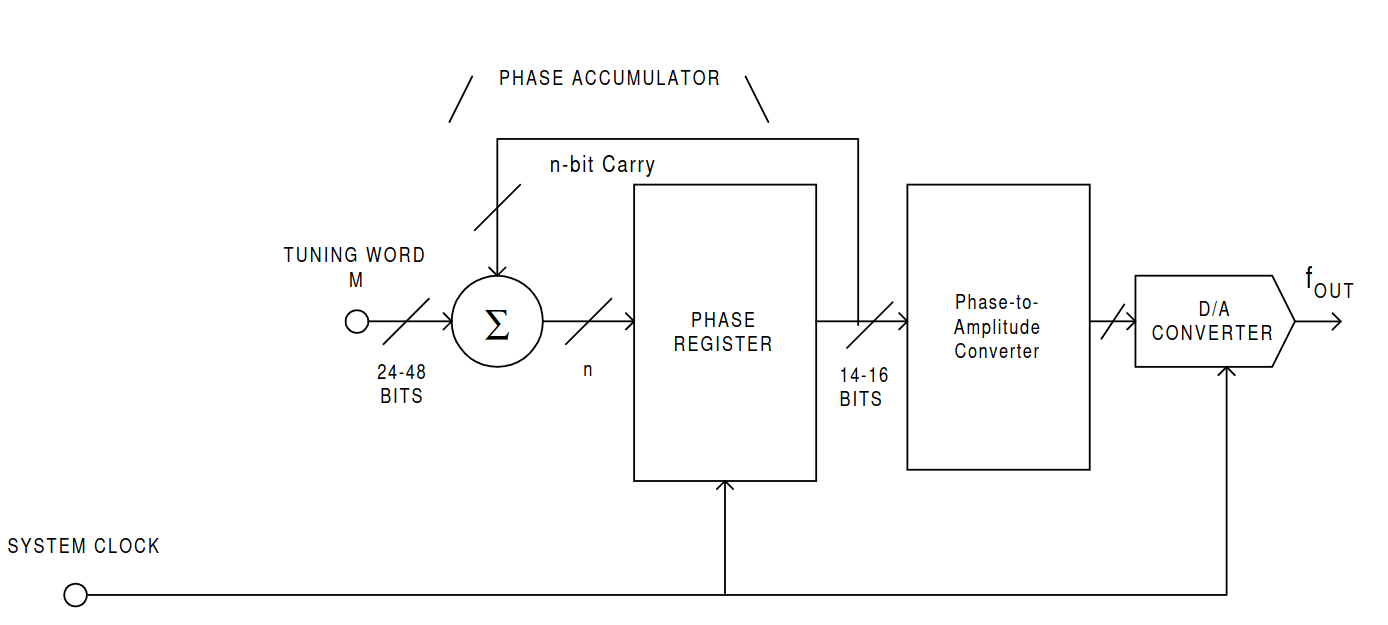
\includegraphics[width=\textwidth]{Setup-software/figures/phase_accumulator_DDS.png}
    \caption[Details of the phase accumulator component of a DDS system]{Details of the phase accumulator component of a DDS system. Credits~\cite{DDS}.}
    \label{fig:phase_accumulator_DDS}
\end{figure}
The address counter is replaced with an N-bit variable-modulus counter and a phase register: effectively storing not a "random" real number, but an integer mapped to a "phase wheel" that indicates the function points to be generated. A typical scheme is presented in \cref{fig:DDS}.

\begin{figure}[ht]
    \centering
    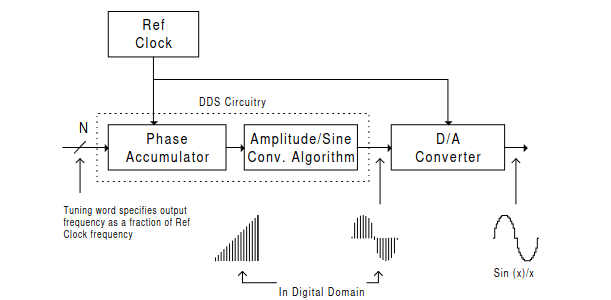
\includegraphics[width=\textwidth]{Setup-software/figures/DDS.png}
    \caption[Scheme of a generic NCO DDS system]{Scheme of a generic NCO DDS system. Credits~\cite{DDS}.}
    \label{fig:DDS}
\end{figure}

This architecture, in respect to the more standard \textit{Phase-Locked Loop} (PLL), offers the advantages of micro-Hertz tuning resolutions, unparalleled matching and control of I-Q synthesized outputs, extremely fast changing speed in frequency and phase.


\subsubsection{Aliasing and synthesis at higher Nyquist zones}\label{sec:aliasing}
Now that we have an idea of the hardware involved for the synthesis, let's try to understand analytically how the DACs behave, how can they be used to synthesize directly in the microwave region, and what are some of the problems involved. 

We can write the output of the DACs as an analytical function~\cite{Kalfus2020}.
Given $f_s$ the sampling frequency, so the rate of conversion from digital samples of a generic analytical function $x(t)$ to analog outputs $v(t)$, we can write:
\begin{equation}\label{eq:v(t)_DAC}
    v(t) = \left[ x(t) \sum^\infty_{k=-\infty} \delta (t - kT) \right] * r(t)
\end{equation}
Where $T=1/f_s$ is the sampling period, inverse of the sampling frequency, and $*$ is the convolution in time operator.
The $r(t)$ function is called \textit{reconstruction waveform} and describes the DAC behaviour between two subsequent samples (so it is non-zero only for $0\le t \le T$).
So, trying to understand \cref{eq:v(t)_DAC}, the summation if a function that is always zero, but in multiples of $T$, where the value between brackets reproduces the $x(t)$ function. Then we have to "connect the dots" to reach an analog continuous function, and this is the role of $*r(t)$.

We now apply Fourier Transform to $v(t)$ to obtain the frequency spectrum (capital functions are the FT of the corresponding time domain function):
\begin{equation*}
    V(\omega) = \mathcal{F}\{v(t)\}=\left[X(\omega) * \mathcal{F} \left\{\sum^\infty_{k=-\infty} \delta (t - kT)  \right\}\right] R(\omega)
\end{equation*}
For the sum we can recognize the $T$ periodicity:
\begin{equation*}
    \sum^\infty_{k=-\infty} \delta (t - kT)  = \sum^\infty_{n=-\infty} c_n e^{2\pi n / T}
\end{equation*}
From $k=0$ we can extract:
\begin{equation*}
    c_n = \frac{1}{T}\int^{T/2}_{T/2} \delta(t) e ^{2\pi n / T}dt = \frac{1}{T}
\end{equation*}
So we can compute the remaining part of FT:
\begin{equation*}
    \mathcal{F} \left\{\sum^\infty_{n=-\infty} \frac{1}{T} e^{2\pi n / T}  \right\} = \frac{1}{T}\sum^\infty_{n=-\infty}\delta (\omega - 2\pi n / T) = \sum^\infty_{n=-\infty} \delta (\omega T - 2\pi n)
\end{equation*}
And finally:
\begin{equation}
    V(\omega) = R(\omega) \left[ X(\omega) * \sum^\infty_{n=-\infty} \delta ( \omega T - 2\pi n) \right]
\end{equation}

The summation represents a series of peaks at multiple of the sampling frequency $f_s$ and the convolution with $X(\omega)$ creates copies of the original signal spectrum at each peak.
If $X(\omega)$ has a bandwidth larger than $f_s/2$ these copies will overlap, leading to a noise phenomenon called \textit{aliasing}.
The frequency bands to be considered, each extending for $f_s/2$, with the first starting at $0$ are called \textit{Nyquist zones}.
So it is not possible to synthesize a signal in a single zone: if $X(\omega)$ is confined in a single one, then every odd zone will have an identical image of the signal, while every even zone will have an inverted image.\\
This is why we generally need to use band pass filters: to exclude the images of spurious Nyquist zones and reduce aliasing effects.

The reconstruction waveform $r(t)$ manifest itself as a frequency-dependant attenuation and different functions will be used for maximize the output power for different Nyquist zones. In particular, the three most common choices are (note that they are all defined in the interval $[0\le t \le T]$):
\begin{description}
    \item[non-return-to-zero (NRZ):] $r(t) = 1\rightarrow R(\omega)=Te^{-i\omega T / 2}\ \frac{\sin\left(\omega T / 2\right)}{\omega T / 2}$
    \item[return-to-zero (RZ):] $r(t) = \theta (-t+0.5T)\rightarrow R(\omega) = \ \frac{T}{2}e^{-i\omega T/4} \ \frac{\sin(\omega T / 4)}{\omega T / 4}$\footnote{$\theta$ is the Heaviside function.}
    \item[mix-mode-rf (MIX):] $r(t) = -sign(t - 0.5T) \rightarrow R(\omega) = \ \frac{\omega T^2}{4}e^{-\ \frac{i}{2}(\omega T - \pi)}\left(\ \frac{\sin(\omega T / 4)}{\omega T / 4}\right)^2$
\end{description}

In \cref{fig:dac-modes} it is shown the attenuation-frequency dependence for different Nyquist zones and different reconstruction waveforms.

\begin{figure}[ht]
    \centering
    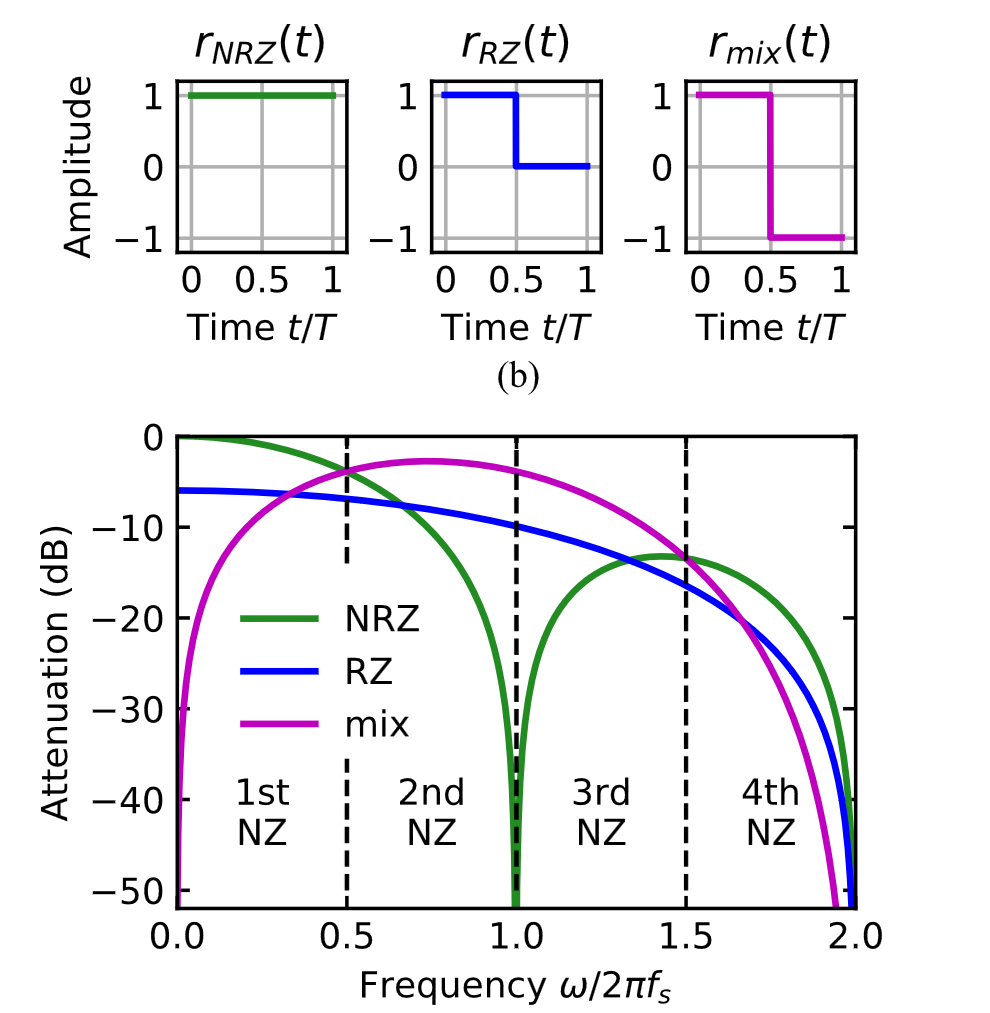
\includegraphics[width=0.6\textwidth]{Setup-software/figures/DAC_modes.png}
    \caption[Attenuation-frequency relationship at different Nyquist zones, for different reconstruction waveforms]{Attenuation-frequency relationship at different Nyquist zones, for different reconstruction waveforms. Credits~\cite{Kalfus2020}.}
    \label{fig:dac-modes}
\end{figure}

The RFSoC-based system that I developed used RNZ for the first Nyquist zone and MIX for all the others.

\subsubsection{Undersampling, decimation and Direct Down Conversion (DDC)}

In last section we saw the main principles and ideas that enable high-performance digital-to-analog conversion, now let's illustrate analog-to-digital.

The starting point for this discussion is the Nyquist-Shannon sampling theorem that establish a sufficient condition for a discrete-time signal to capture all the information contained in a continuous-tine signal.
Without entering in any details regarding the mathematical demonstration, we can express the theorem as\footnote{This theorem is often simply referred to as Nyquist sampling theorem.}:
\begin{theorem}
    If a function $x(t)$ does not contain any frequencies higher than $M$ Hz, then it can be completely described by finite samples spaced less than $1/(2M)$ s.
\end{theorem}
So, a signal must be sampled at a rate greater than twice its maximum frequency in order to assure complete and unambiguous reconstruction.
In general, the effect of not meeting the Nyquist-Shannon criterion is again aliasing.\\
Sampling with a frequency $\ge 2M$ is called \textit{normal sampling} or \textit{oversampling}.

If we use sampling frequency that are less than twice the maximum frequency than we use \textit{undersampling}.
Here we have another theorem, also called Nyquist-Shannon sampling theorem:
\begin{theorem}
    If a function $x(t)$ has a bandwidth of $B$ Hz, then it can be completely described by finite samples spaced less than $1/(2B)$ s.
\end{theorem}
The two theorems are similar, but note that they apply at the same time, so we will have aliasing.
While aliasing usually is a non-desired effect, with undersampling we try to exploit it.
The aliased signal always appear at:
\begin{equation}\label{eq:undersampling}
    f_{ADC} = f_s - f_{in}
\end{equation}
where $f_s$ is the sampling frequency, $f_{in}$ the input frequency and $f_{ADC}$ the acquired one.
If we know in advance that the signal is aliased, than we can easily recover the actual frequencies using the inverse of \cref{eq:undersampling}.

Since in our system we are acquiring a reflected/transmitted signal that was produces by us, we know exactly what frequencies we have in input and is very easy to reconstruct the signal.
Also note that the undersampling technique has several advantages:
\begin{itemize}
    \item higher sampling rate increases data rates to FPGAs and this can deteriorate performances or increase the cost of the FPGAs;
    \item higher data rates usually need more time to setup, meaning larger dead times;
    \item higher sampling rate are linked to higher power consumption;
    \item to reach a situation where the Nyquist-Shannon criterion is met we usually need to involve external Local Oscillators and Mixing, that are not needed for undersampling.
\end{itemize}

And there are also some disadvantages:
\begin{itemize}
    \item worse S/N ratios~\footnote{The Signal-to-Noise Ratio (S/N ratio) is a measure used in signal processing and communication systems to quantify the relative levels of a desired signa to unwanted background noise. It is typically expressed in decibels (dB) and is calculated as: \[ \text{S/N ratio (dB)} = 10 \cdot \log_{10}\left(\frac{P_{\text{signal}}}{P_{\text{noise}}}\right) \] Where: \(P_{\text{signal}}\) is the power of the signal (the strength of the desired information-carrying component of the signal) and \(P_{\text{noise}}\) is the power of the noise (the unwanted or interfering components of the signal, typically background or random variations).};
    \item we need to plan in advance what frequency we want to sample, otherwise we will not be able to directly apply \cref{eq:undersampling};
    \item undersampling cannot be used to sample high signal bandwidths.
\end{itemize}

The RFSoC-base system developed in this thesis used the undersampling, with the great advantage of not requiring external local oscillator.

Moreover, at the output of each ADC, internally to the FPGA logic, another operation was conducted: an eight-time \textit{decimation}.
The idea of decimation is that it is inefficient to transmit a wideband spectrum when only a narrow band is required, so we conserve only a small periodic portion of the ADC samples.
The results is to effectively reducing the sample rate of the ADC: for our system, a decimation by 8 means that $7/8$ of the total samples were completely discarded.\\
The ADC also contains a NCO and a digital filters that remove the out-of-band noise.

All this system, that can usually be called \textit{Digital Down Conversion} (DDC) in analogy with DDS preserves all the information in the frequency band of interest, while also removing much all noise at different frequencies.\\
In the RFSoC-base system for quantum control it will be used to efficiently acquire complex (I-Q) samples.

\subsubsection{Used RFSoC boards}

The system for quantum control and readout that was developed during this thesis can in theory be used without any modification with all the boards supported by the \Qick~\cite{Stefanazzi2022} package: a firmware and software library developed at Fermilab for using RFSoC boards for quantum computing.
However, all the results produced and experiment conducted where obtained using a \RFSoC and a \ZCU (for some part of the thesis I also worked with a \textbf{ZCU216} which shares the main characteristics with the \ZCU).
Some details about these boards are presented in \cref{tab:used_rfsocs}.

\begin{table}[ht]
    \centering
    \begin{tabular}{llll}
                            & RFSoC4x2            & ZCU111               & ZCU216 \\ \hline
    Number of ADCSs         & 4 (1 used)          & 8 (2 used)           & 16 (2)      \\
    Number of DACs          & 2                   & 8                    & 16          \\
    DAC sampling frequency  & 9.85 GSPS           & 6.55 GSPS            & 9.85 GSPS   \\
    ADC sampling frequency  & 5.00 GSPS           & 4.09 GSPS            & 2.5 GSPS    \\
    Chip generation         & third gen.          & first gen.           & third gen.  \\
    \end{tabular}
    \caption[Characteristics of the supported RFSoCs]{Outline of the main characteristics of the \RFSoC, \ZCU and \textbf{ZCU216} boards.}
    \label{tab:used_rfsocs}
\end{table}
Both of these boards have Ethernet connectors so they were always controlled over the internet.

\begin{figure}[ht]
    \centering
    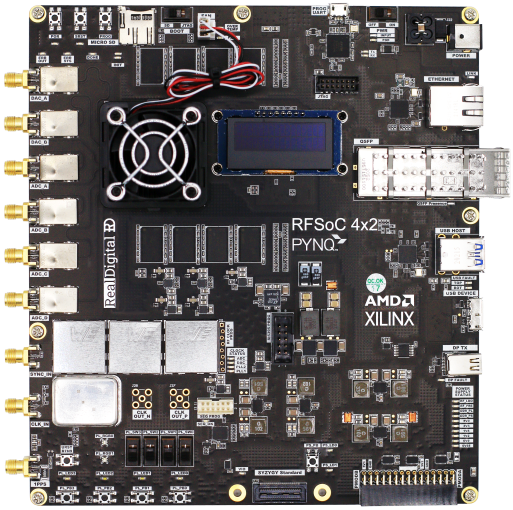
\includegraphics[width=0.6\textwidth]{Setup-software/figures/rfsoc4x2.png}
    \caption{Picture of a RFSoC4x2 board.}
    \label{fig:rfsoc4x2}
\end{figure}

The \RFSoC is much smaller than the \ZCU, while it is smaller, the \RFSoC is a FPGA of third generation, meaning it has much higher sampling frequencies.
Since there are just two DACs, this board can be used to control a single non-flux-tunable qubit. The connections will be:
\begin{itemize}
    \item \textbf{DAC 1:} drive line
    \item \textbf{DAC 2:} readout line
    \item \textbf{ADC 1:} feedback line (for readout)
    \item \textbf{ADC 2:} not active
    \item \textbf{ADC 3:} not active
    \item \textbf{ADC 4:} not active
\end{itemize}
As visible in \cref{fig:rfsoc4x2} \RFSoC has direct connections to SMA cables so it does not require any specific additional connector.
By \textit{not active} I mean that the firmware used never activates it; a different firmware potentially could.

On the other hand, the \ZCU board is a bit more complex. As is visible in \cref{fig:zcu111} there are no SMA connectors and an additional board is needed to convert from the black band connectors (the two band on the left in the figure) to SMAs.
\begin{figure}[ht]
    \centering
    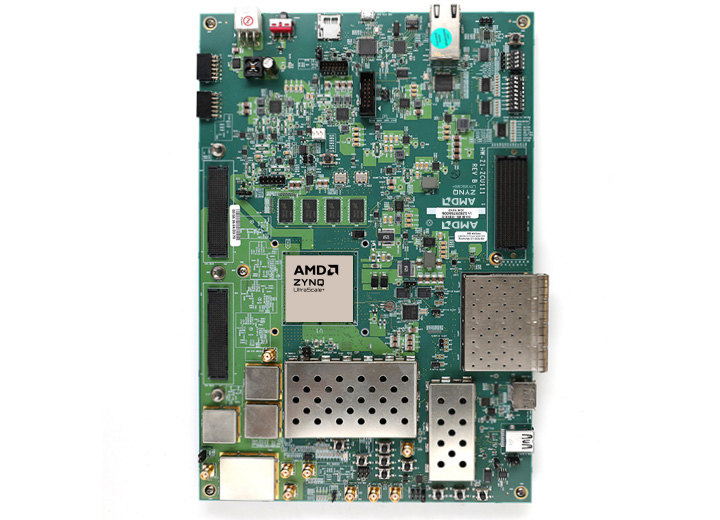
\includegraphics[width=\textwidth]{Setup-software/figures/zcu111.jpg}
    \caption{Picture of a ZCU111 board.}
    \label{fig:zcu111}
\end{figure}

Fortunately, with the \ZCU is sold by default a \textbf{XM500} board, shown in \cref{fig:xm500}.\\
Unfortunately, the \textbf{XM500} board is not just a convertor, but also adds some filtering and changes the output in non trivial ways.
\begin{figure}[ht]
    \centering
    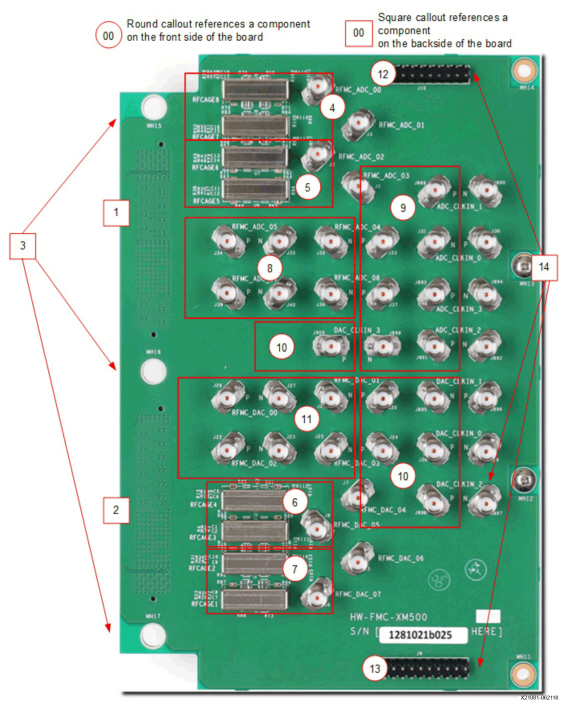
\includegraphics[width=0.65\textwidth]{Setup-software/figures/xm500.jpeg}
    \caption{Picture of a XM500 board.}
    \label{fig:xm500}
\end{figure}
In particular, the \textbf{XM500} has:
\begin{itemize}
    \item \textbf{external clock inputs/outputs:} not active;
    \item \textbf{4 single output DACs:} these are all active, but they have a balun filter added to it. That is a high-pass filter that removes DC components. So these cannot be used for DC flux control;
    \item \textbf{2 ADC:} active and also with baluns (but there are no downsides here);
    \item \textbf{3 differential output DACs:} these do not have baluns, so they can be used for flux lines, but require specific differential amplifiers to subtract the two outputs to convert them to a single SMA (also, the vast majority of differential amplifiers does not work for DC signals).
\end{itemize}

For the \ZCU, the \Qick project offers two different firmwares: one uses both ADCs, so can be used to control up to two flux-tunable qubits, the other uses a single ADC multiplexed.
The multiplex firmware is of particular interest and has been extensively used during the thesis.
Loading it, one of the DACs become capable of sending 4 different pulses at different frequencies but at the same time, while one of the ADC becomes capable of acquiring 4 different pulses (again at 4 different frequencies) at the same time.

This is one of the perks of using a re-configurable FPGA: since the ADCs and DACs are products of the FPGA logic is possible to reconfigure them so that a single ADC is actually composed of 4 with smaller bandwidth.\\
For this configuration, anyway, we used a standard upconversion system for the DAC so that, even with a smaller $f_s$, the output was in the first Nyquist zone (for power reasons).


\subsection{Qubits Configuration}

At TII, the XLD cryostat was used at its full capacity and contained, at the mixing chamber level:
\begin{itemize}
    \item 3 single non-flux-tunable qubit manufactured by TII, in custom 3D cavities;
    \item a 5 flux-tunable qubits chip, with a star connectivity (namely a single qubit in the middle that can couple to the other four);
    \item a 5 flux-tunable qubits with couplers (namely flux-tunable qubits between other qubits, used to mediate the interaction between the two qubits);
    \item  a 25 qubit chip with 5 readout lines and various qubits connected to each other.
\end{itemize}

In the work for this thesis, I tested and interacted, in particular, with the single qubit devices and one readout line of the 25 qubit chip.

The single qubits, that were changed and replaced over my period at TII, generally share the same schematic and the reader can imagine them as presented in \cref{fig:single_qubit}.

\begin{figure}[ht]
    \centering
    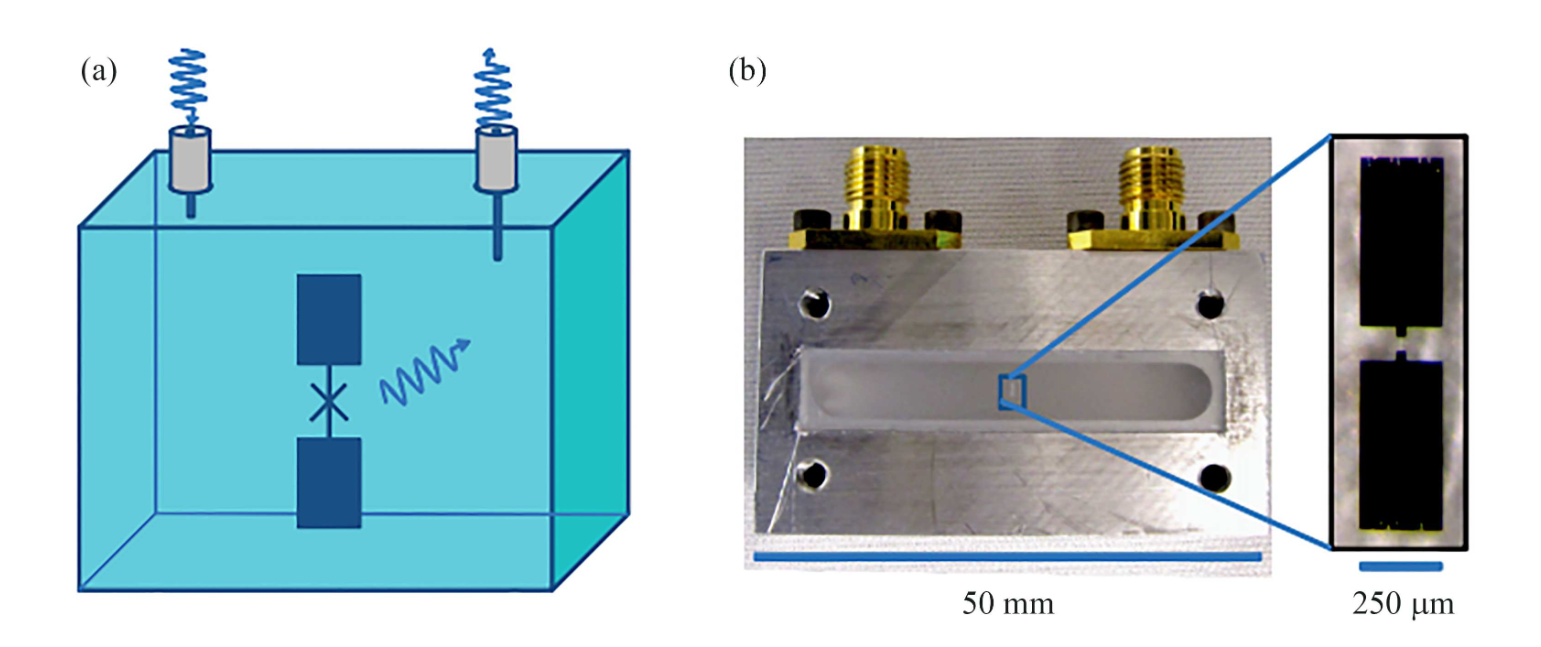
\includegraphics[width=\textwidth]{Setup-software/figures/ex:transmon.png}
    \caption[Example of a single qubit in a 3D cavity]{Example of a single qubit in a 3D cavity. Credits~\cite{Huang2020}.}
    \label{fig:single_qubit}
\end{figure}

\begin{figure}[ht]
    \centering
    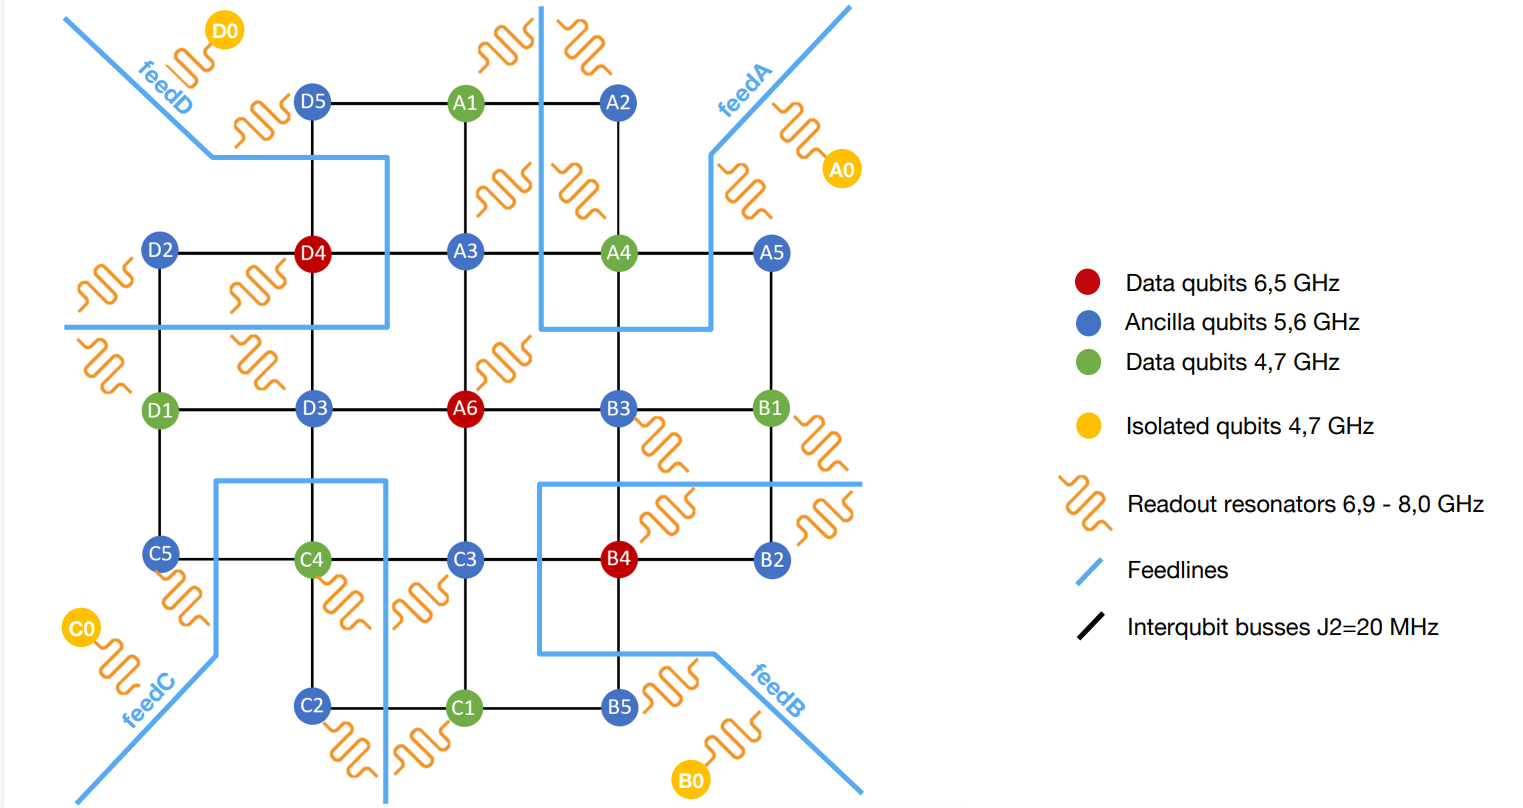
\includegraphics[width=0.8\textwidth]{Setup-software/figures/contralto.png}
    \caption[Topology of the Contralto QuatWare chip]{Topology of the Contralto QuatWare chip. Credits~\cite{contralto}.}
    \label{fig:contraltro_chip}
\end{figure}
The 25 qubits chip is schematically presented in \cref{fig:contraltro_chip}

Among all the present qubits, the \ZCU was connected to line D.\\
Note that every line has 5 qubits plus an isolated one (the yellows) that are qubit used only for testing.\\
Moreover, all the black interconnecting lines are possible two-qubits gates.


\subsection{Configuration and setup for RFSoC4x2}

During this thesis work, the \RFSoC was connected to multiple single qubit in 3D cavities.
Therefore, the setup changed several times, but it always had some stable attributes.
For example, in a single qubit (transmon) non flux tunable, there is only a single line for input (were both readout and drive pulses are fired) and a single readout output (\textit{feedback}).

\begin{figure}[ht]
    \centering
    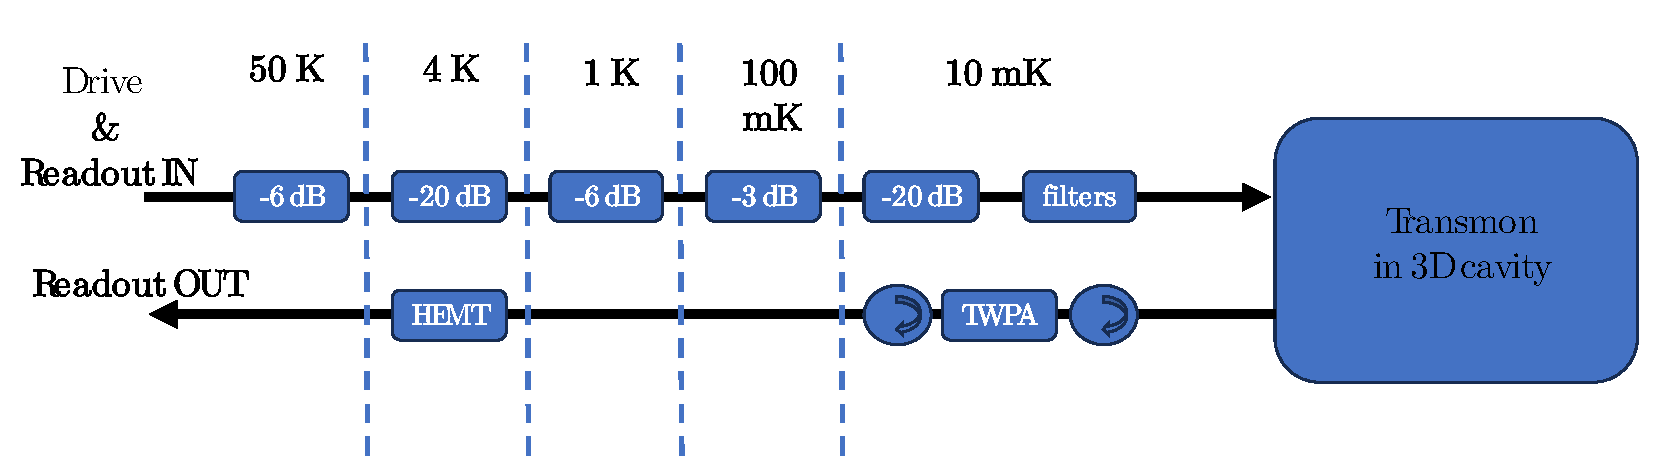
\includegraphics[width=\textwidth]{Setup-software/figures/scheme_lines_single.pdf}
    \caption{Schematics of the lines of a single non-flux-tunable qubit in a 3D cavity.}
    \label{fig:lines_single}
\end{figure}

In \cref{fig:lines_single} the two lines (in-fridge) are presented.
All the attenuation present in the IN line is needed to help to reach the single-photon level (or near-single-photon) and its spread to avoid excessive thermal load to a specific stage of the dilution.\\
The filters represented at the mixing chamber level included both IR filter and low-pass filters to clean in the best possible way any noise.

In the readout OUT line, the first element is TWPA~\cite{Yaakobi2013} manufactured by Silent Waves~\cite{silentwaves} continuously pumped (with another line not present in the scheme) during the experiments.
The role of the TWPA is to amplify the signal, inducing a noise amplification quantum limited.
Note that the TWPA was not present in the majority of the setups, but is inserted in the scheme for completeness.\\
At the $4$ K level, a cryogenic HEMT~\cite{Baulieu2022} is present so that the signal, extremely low in the input, becomes measurable.

At room temperature the \textit{feedback signal} is amplified with a LNA (Low Noise Amplifier) manufactured by MiniCircuit~\cite{minicircuit} (max $+8$ dB ) and sent to the \RFSoC ADC 0.\\
The drive source is DAC 0 (B on the board) and sometimes an amplification of max $+8$ dB was needed.
The readout IN was connected to DAC 1 (A on the board) and merged to the drive by using a passive \textit{splitter}.\\
At room temperature, some band-pass filters were added to remove spurious created by the synthesis process and eventual high frequency noise.


\subsection{Configuration and setup for ZCU111}

Similarly as per single qubit control, in \cref{fig:lines_zcu} are showed the in-fridge lines for the control of the multiplexed qubits of the 25 qubits chip. 

\begin{figure}[ht]
    \centering
    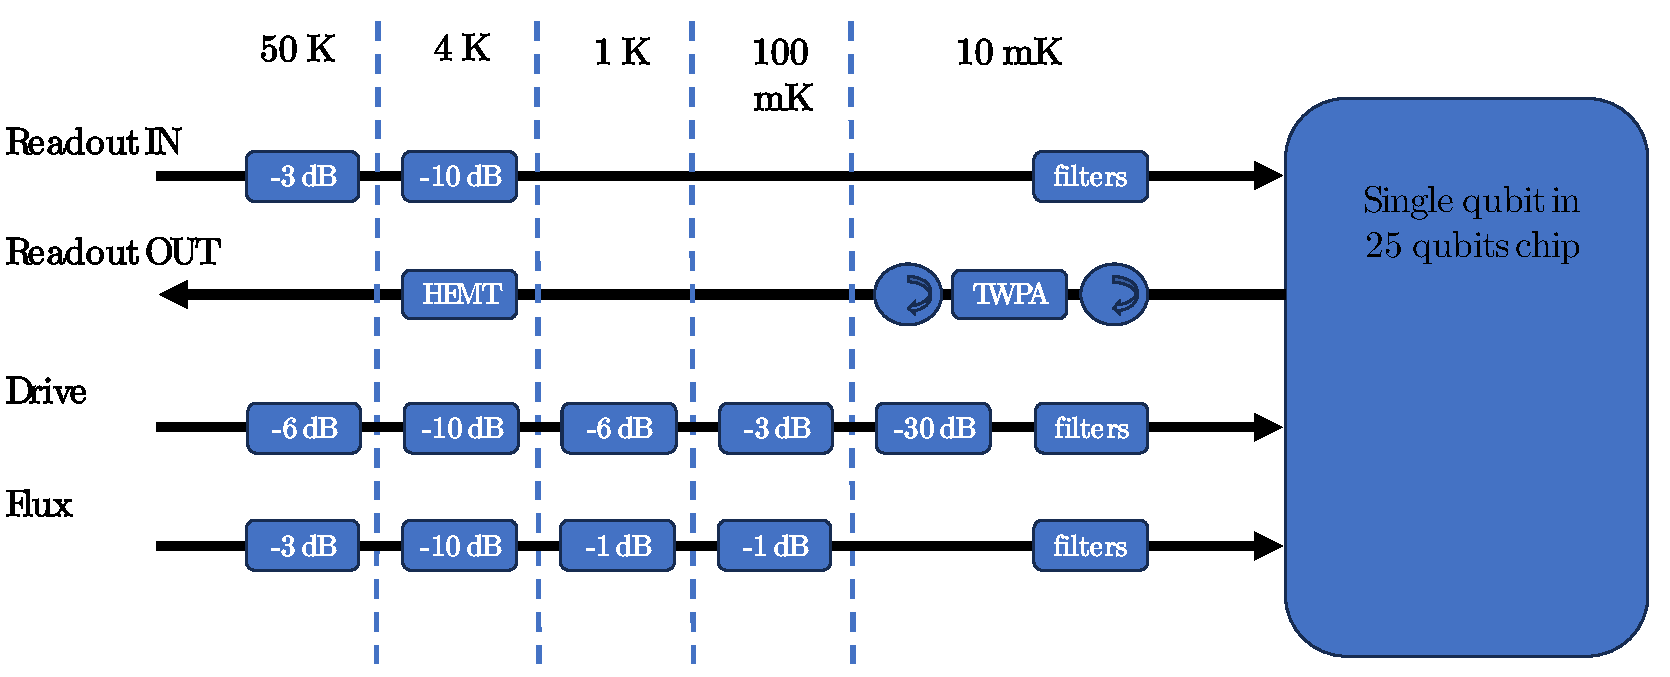
\includegraphics[width=\textwidth]{Setup-software/figures/scheme_lines_25.pdf}
    \caption{Schematics of the lines of a single flux-tunable qubit in the 25 qubit chip.}
    \label{fig:lines_zcu}
\end{figure}

Note first that there are multiple input lines and, in particular, that the readout in and the drive line are are separated.
This is mainly because this is a 2D chip and not a cavity.\\
In any case, both for the readoutIN and the drive the filters are the same already named in the single qubit setup.

For the flux line, on the other hand, the filters are extremely low frequency filters since in theory we just need a DC current.

The TWPA is one of the differing elements. In fact it was not used a standard fixed-band TWPA as per the single qubit setup, but a prototype of a variable-band TWPA~\cite{Ranadive2022}.
This TWPA needs a pump to work and a DC current to tune the amplification band and gain. Both these lines are not showed in the scheme since they are more or less secondary.

Some more differences are present at room temperature, where the setup is a bit more complex.
In particular note that the schematics presented in \cref{fig:lines_zcu} represent a single qubit, but this is a system with 5+1 multiplexed qubits.
Therefore, at room temperature we will have the DAC 6 of the \ZCU connected to the readoutIN while a mux firmware is loaded.
This basically cause the bandwidth to go from $6$ GHz to few MHz, is therefore required a local oscillator with an up-conversion scheme as presented in \cref{fig:up-down-conversion}. 
\begin{figure}[ht]
    \centering
    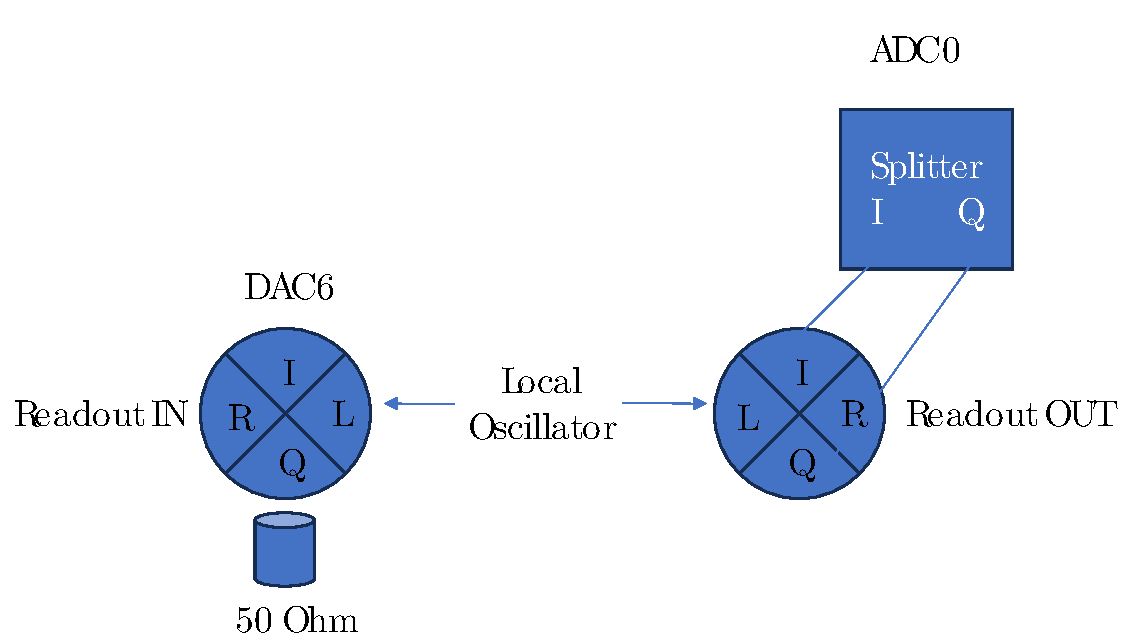
\includegraphics[width=0.7\textwidth]{Setup-software/figures/upconversion.pdf}
    \caption{Scheme used for down and up-conversion.}
    \label{fig:up-down-conversion}
\end{figure}
As it shown, the same local oscillator is also used for down-conversion.
Since this process uses an IQ mixer, in the down-conversion I and Q are splitted and gets merged back again using a splitter connected to the board ADC 0.

For the drive lines is sometimes needed additional amplification that was provided through a LNA.
They were connected to DAC 3-4-5 to achieve full control of 3 qubits at the same time.

For the flux lines some more work is needed since the outputs of the companion XM500 board (that exposes the SMA connections) have baluns (i.e. DC filters) on its single-ended connection.
There are two option to proceed: it is possible to buy/project a new companion boards or to leverage the 3 differential outputs of the XM500.
This second option was chosen for simplicity.
Note that the differential outputs P-N can be merged together via a simple subtraction P-N, something that standard differential amplifiers easily do, but that since we are aiming for DC currents these are not an option because they use capacitors and operates as high-pass filters.
Special active differential amplifiers are needed in this case.\\
Having bought 3 of them, we were able to bias 3 flux-tunable qubits using DACs 0-1-2.

\subsection{Configuration and setup for ZCU216}

The \textbf{ZCU216} was used with the same setup composed for the \textbf{ZCU111}.
This was a temporary solution that was also limiting the board potential.

In particular, the \textbf{ZCU216} could potentially be used to fully control 7 flux tunable qubits (considering 7 drive lines, 7 flux lines and a maximum of 2 readout inputs), while with the used scheme only three qubits were usable.
To fully unblock the board potential, however, it is needed to make some changes to the \Qick firmware and this requires particular work.


%\subsection{FPGA \& RFSoC}

A Field-Programmable Gate Array (FPGA) is an electronic board that supports complete firmware configuration \textit{after} manufacturing as well as partial re-configurations while executing a specific program.\\
While integrated circuits serve a specific purpose and cannot be re-configured after fabrication, FPGAs can contain arrays of programmable logic blocks that can serve simple logic purposes (as Boolean operations) or complex functions, depending on the loaded firmware.
Since they are completely re-configurable and since they can improve the performance of standard CPU (with task-specific firmwares) without the large energy conception required by GPUs, FPGAs are rapidly becoming of widespread use.
Moreover, since the same FPGA can serve different purposes in extremely different fields, it is usually a cheap alternative to standard systems.\\
The drawback of all of this is in the overhead that programming a FPGA introduces.
To compile a FPGA firmware one first has to define the logic to use via Hardware Description Languages (HDL) then design the connections internal to the FPGA logic and conduct precise tests on the produced firmware.

The type of FPGAs used in my thesis are RFSoC, namely Radio Frequency System on Chip: their main characteristic is the capability of synthesizing directly frequency up to $\approx 10$ GHz, as well as the capability of acquiring extremely high frequency by exploiting the downsampling technique. 
All of this combined in the same board, along with a standard CPU, RAM and memory: enabling the creation of a full on-board system.\\
In this section I will provide some explanation on the techniques used for high-frequency synthesis and high frequency acquisition. 
Also, some details on the FPGAs used will be provided.

\subsubsection{Direct Digital Synthesis (DDS)}
The technique used for direct microwave synthesis is called \textit{Direct Digital Synthesis} (DDS) and it enables to use the DACs as arbitrary waveform generators for high frequencies~\cite{DDS}.

In general, a DDS system consist in a precision reference clock (often a crystal clock), an address counter, a programmable read-only memory (PROM) and a DAC (see \cref{fig:simple_DDS} for reference).\\
In the PROM, a complete cycle of a periodic function is stored and the address counter steps through it, accessing sequentially  all the PROMS's memory locations (so the PROM is working a lookup table).
The DAC then converts the input from the PROM, to analog outputs.

Note also that the PROM can be composed of two different lookup tables, for complex I-Q signals, often referred to "in-phase and quadrature signals," are a pair of time-varying signals used in signal processing and communications. They represent:
\begin{description}
    \item[In-Phase (I) Component] The "I" component represents the signal's amplitude or phase information. It corresponds to the real part of the complex signal.
    \item[Quadrature (Q) Component] The "Q" component is also a real part of the complex signal but is phase-shifted by 90 degrees relative to the "I" component. The "Q" component carries information orthogonal to that of the "I" component.
\end{description}


\begin{figure}[ht]
    \centering
    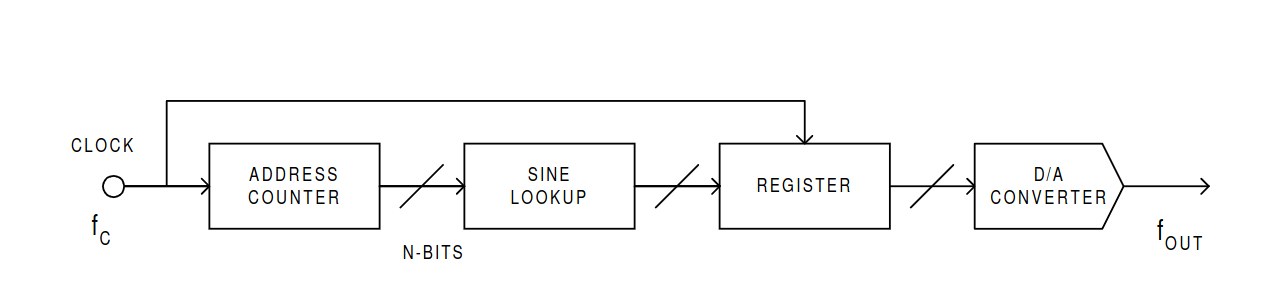
\includegraphics[width=\textwidth]{Setup-software/figures/simple_DDS.png}
    \caption{A simple Direct-Digital-Synthesizer, where the function stored in PROM is a sine wave. Credits~\cite{DDS}.}
    \label{fig:simple_DDS}
\end{figure}

This implementation of DDS is a bit simplified and, although it works, it lacks tuning flexibility and the output frequency is effectively fixed to the reference clock one.\\
A modern DDS system adds to the shown signal chain a phase accumulator, creating an architecture usually referred to as numerically-controlled oscillator NCO (see \cref{fig:phase_accumulator_DDS}).
\begin{figure}[ht]
    \centering
    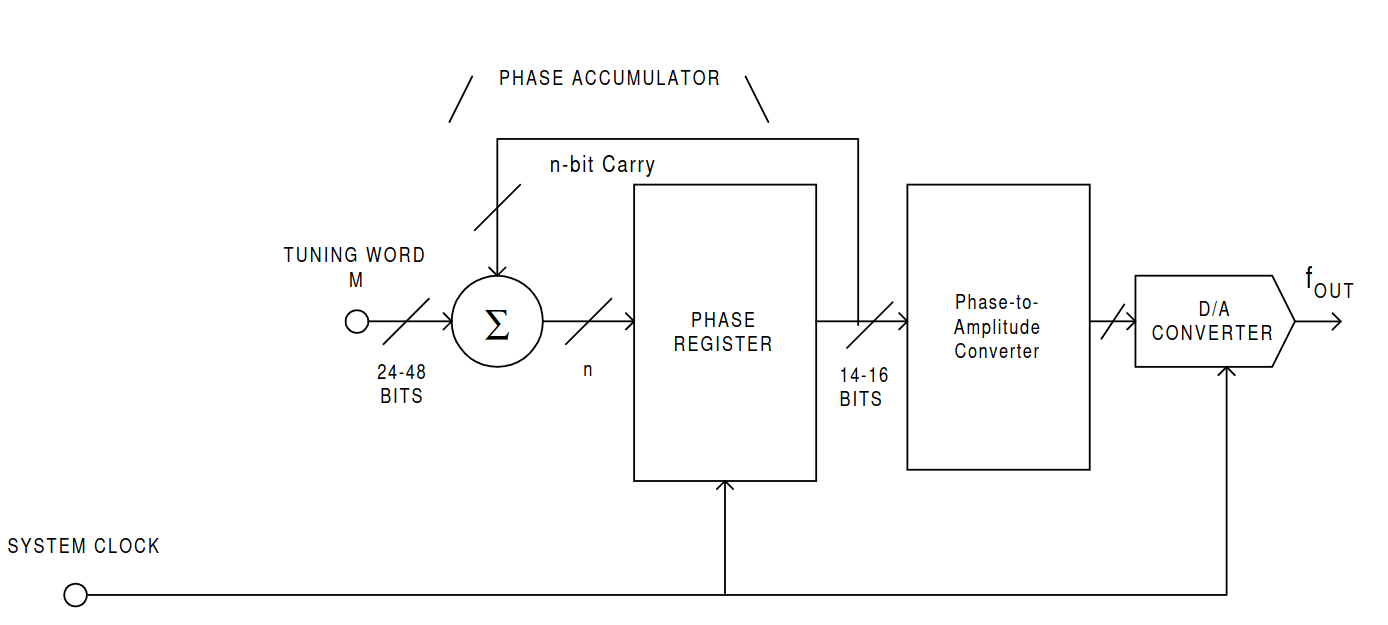
\includegraphics[width=\textwidth]{Setup-software/figures/phase_accumulator_DDS.png}
    \caption[Details of the phase accumulator component of a DDS system]{Details of the phase accumulator component of a DDS system. Credits~\cite{DDS}.}
    \label{fig:phase_accumulator_DDS}
\end{figure}
The address counter is replaced with an N-bit variable-modulus counter and a phase register: effectively storing not a "random" real number, but an integer mapped to a "phase wheel" that indicates the function points to be generated. A typical scheme is presented in \cref{fig:DDS}.

\begin{figure}[ht]
    \centering
    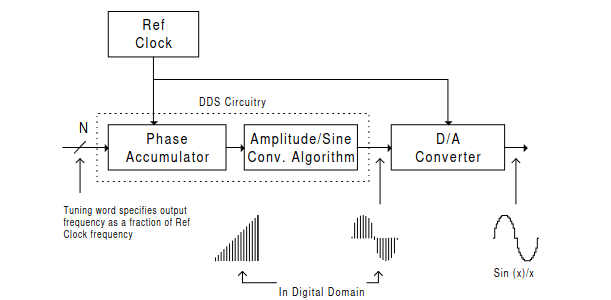
\includegraphics[width=\textwidth]{Setup-software/figures/DDS.png}
    \caption[Scheme of a generic NCO DDS system]{Scheme of a generic NCO DDS system. Credits~\cite{DDS}.}
    \label{fig:DDS}
\end{figure}

This architecture, in respect to the more standard \textit{Phase-Locked Loop} (PLL), offers the advantages of micro-Hertz tuning resolutions, unparalleled matching and control of I-Q synthesized outputs, extremely fast changing speed in frequency and phase.


\subsubsection{Aliasing and synthesis at higher Nyquist zones}\label{sec:aliasing}
Now that we have an idea of the hardware involved for the synthesis, let's try to understand analytically how the DACs behave, how can they be used to synthesize directly in the microwave region, and what are some of the problems involved. 

We can write the output of the DACs as an analytical function~\cite{Kalfus2020}.
Given $f_s$ the sampling frequency, so the rate of conversion from digital samples of a generic analytical function $x(t)$ to analog outputs $v(t)$, we can write:
\begin{equation}\label{eq:v(t)_DAC}
    v(t) = \left[ x(t) \sum^\infty_{k=-\infty} \delta (t - kT) \right] * r(t)
\end{equation}
Where $T=1/f_s$ is the sampling period, inverse of the sampling frequency, and $*$ is the convolution in time operator.
The $r(t)$ function is called \textit{reconstruction waveform} and describes the DAC behaviour between two subsequent samples (so it is non-zero only for $0\le t \le T$).
So, trying to understand \cref{eq:v(t)_DAC}, the summation if a function that is always zero, but in multiples of $T$, where the value between brackets reproduces the $x(t)$ function. Then we have to "connect the dots" to reach an analog continuous function, and this is the role of $*r(t)$.

We now apply Fourier Transform to $v(t)$ to obtain the frequency spectrum (capital functions are the FT of the corresponding time domain function):
\begin{equation*}
    V(\omega) = \mathcal{F}\{v(t)\}=\left[X(\omega) * \mathcal{F} \left\{\sum^\infty_{k=-\infty} \delta (t - kT)  \right\}\right] R(\omega)
\end{equation*}
For the sum we can recognize the $T$ periodicity:
\begin{equation*}
    \sum^\infty_{k=-\infty} \delta (t - kT)  = \sum^\infty_{n=-\infty} c_n e^{2\pi n / T}
\end{equation*}
From $k=0$ we can extract:
\begin{equation*}
    c_n = \frac{1}{T}\int^{T/2}_{T/2} \delta(t) e ^{2\pi n / T}dt = \frac{1}{T}
\end{equation*}
So we can compute the remaining part of FT:
\begin{equation*}
    \mathcal{F} \left\{\sum^\infty_{n=-\infty} \frac{1}{T} e^{2\pi n / T}  \right\} = \frac{1}{T}\sum^\infty_{n=-\infty}\delta (\omega - 2\pi n / T) = \sum^\infty_{n=-\infty} \delta (\omega T - 2\pi n)
\end{equation*}
And finally:
\begin{equation}
    V(\omega) = R(\omega) \left[ X(\omega) * \sum^\infty_{n=-\infty} \delta ( \omega T - 2\pi n) \right]
\end{equation}

The summation represents a series of peaks at multiple of the sampling frequency $f_s$ and the convolution with $X(\omega)$ creates copies of the original signal spectrum at each peak.
If $X(\omega)$ has a bandwidth larger than $f_s/2$ these copies will overlap, leading to a noise phenomenon called \textit{aliasing}.
The frequency bands to be considered, each extending for $f_s/2$, with the first starting at $0$ are called \textit{Nyquist zones}.
So it is not possible to synthesize a signal in a single zone: if $X(\omega)$ is confined in a single one, then every odd zone will have an identical image of the signal, while every even zone will have an inverted image.\\
This is why we generally need to use band pass filters: to exclude the images of spurious Nyquist zones and reduce aliasing effects.

The reconstruction waveform $r(t)$ manifest itself as a frequency-dependant attenuation and different functions will be used for maximize the output power for different Nyquist zones. In particular, the three most common choices are (note that they are all defined in the interval $[0\le t \le T]$):
\begin{description}
    \item[non-return-to-zero (NRZ):] $r(t) = 1\rightarrow R(\omega)=Te^{-i\omega T / 2}\ \frac{\sin\left(\omega T / 2\right)}{\omega T / 2}$
    \item[return-to-zero (RZ):] $r(t) = \theta (-t+0.5T)\rightarrow R(\omega) = \ \frac{T}{2}e^{-i\omega T/4} \ \frac{\sin(\omega T / 4)}{\omega T / 4}$\footnote{$\theta$ is the Heaviside function.}
    \item[mix-mode-rf (MIX):] $r(t) = -sign(t - 0.5T) \rightarrow R(\omega) = \ \frac{\omega T^2}{4}e^{-\ \frac{i}{2}(\omega T - \pi)}\left(\ \frac{\sin(\omega T / 4)}{\omega T / 4}\right)^2$
\end{description}

In \cref{fig:dac-modes} it is shown the attenuation-frequency dependence for different Nyquist zones and different reconstruction waveforms.

\begin{figure}[ht]
    \centering
    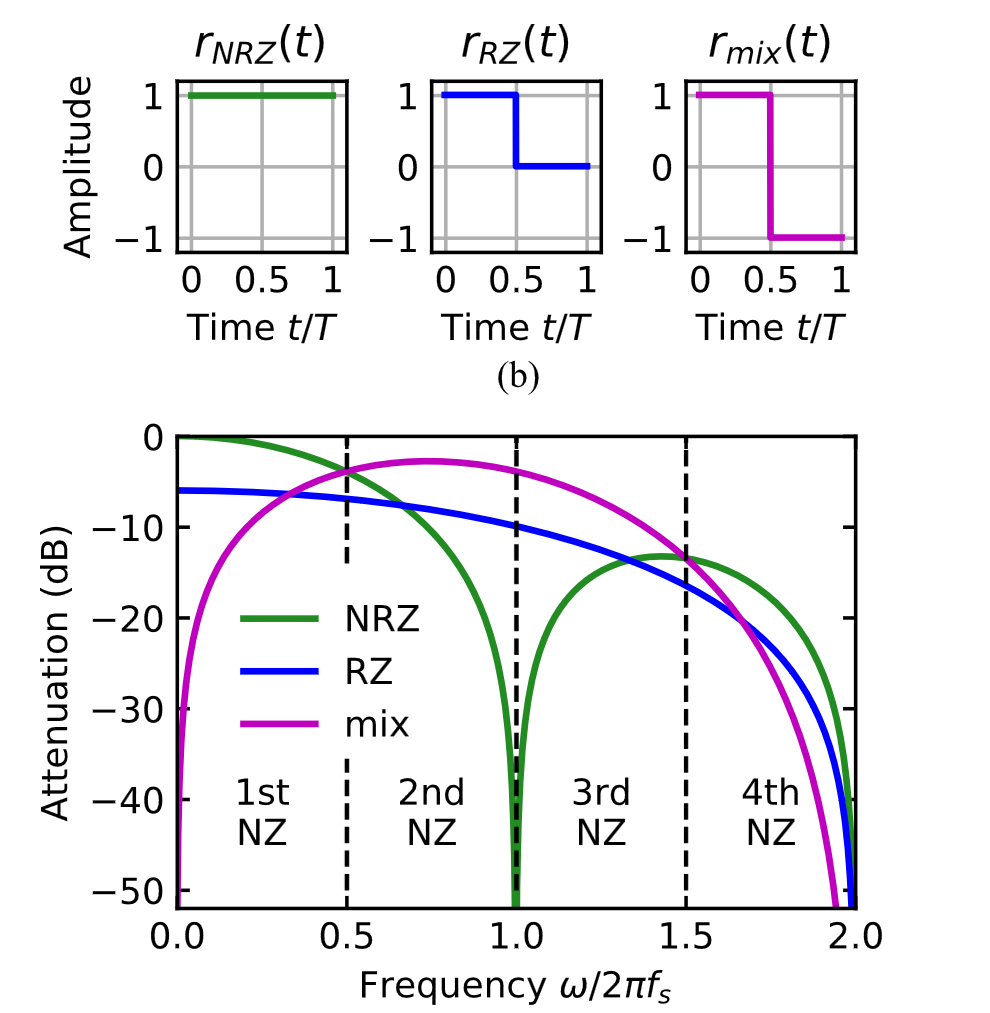
\includegraphics[width=0.6\textwidth]{Setup-software/figures/DAC_modes.png}
    \caption[Attenuation-frequency relationship at different Nyquist zones, for different reconstruction waveforms]{Attenuation-frequency relationship at different Nyquist zones, for different reconstruction waveforms. Credits~\cite{Kalfus2020}.}
    \label{fig:dac-modes}
\end{figure}

The RFSoC-based system that I developed used RNZ for the first Nyquist zone and MIX for all the others.

\subsubsection{Undersampling, decimation and Direct Down Conversion (DDC)}

In last section we saw the main principles and ideas that enable high-performance digital-to-analog conversion, now let's illustrate analog-to-digital.

The starting point for this discussion is the Nyquist-Shannon sampling theorem that establish a sufficient condition for a discrete-time signal to capture all the information contained in a continuous-tine signal.
Without entering in any details regarding the mathematical demonstration, we can express the theorem as\footnote{This theorem is often simply referred to as Nyquist sampling theorem.}:
\begin{theorem}
    If a function $x(t)$ does not contain any frequencies higher than $M$ Hz, then it can be completely described by finite samples spaced less than $1/(2M)$ s.
\end{theorem}
So, a signal must be sampled at a rate greater than twice its maximum frequency in order to assure complete and unambiguous reconstruction.
In general, the effect of not meeting the Nyquist-Shannon criterion is again aliasing.\\
Sampling with a frequency $\ge 2M$ is called \textit{normal sampling} or \textit{oversampling}.

If we use sampling frequency that are less than twice the maximum frequency than we use \textit{undersampling}.
Here we have another theorem, also called Nyquist-Shannon sampling theorem:
\begin{theorem}
    If a function $x(t)$ has a bandwidth of $B$ Hz, then it can be completely described by finite samples spaced less than $1/(2B)$ s.
\end{theorem}
The two theorems are similar, but note that they apply at the same time, so we will have aliasing.
While aliasing usually is a non-desired effect, with undersampling we try to exploit it.
The aliased signal always appear at:
\begin{equation}\label{eq:undersampling}
    f_{ADC} = f_s - f_{in}
\end{equation}
where $f_s$ is the sampling frequency, $f_{in}$ the input frequency and $f_{ADC}$ the acquired one.
If we know in advance that the signal is aliased, than we can easily recover the actual frequencies using the inverse of \cref{eq:undersampling}.

Since in our system we are acquiring a reflected/transmitted signal that was produces by us, we know exactly what frequencies we have in input and is very easy to reconstruct the signal.
Also note that the undersampling technique has several advantages:
\begin{itemize}
    \item higher sampling rate increases data rates to FPGAs and this can deteriorate performances or increase the cost of the FPGAs;
    \item higher data rates usually need more time to setup, meaning larger dead times;
    \item higher sampling rate are linked to higher power consumption;
    \item to reach a situation where the Nyquist-Shannon criterion is met we usually need to involve external Local Oscillators and Mixing, that are not needed for undersampling.
\end{itemize}

And there are also some disadvantages:
\begin{itemize}
    \item worse S/N ratios~\footnote{The Signal-to-Noise Ratio (S/N ratio) is a measure used in signal processing and communication systems to quantify the relative levels of a desired signa to unwanted background noise. It is typically expressed in decibels (dB) and is calculated as: \[ \text{S/N ratio (dB)} = 10 \cdot \log_{10}\left(\frac{P_{\text{signal}}}{P_{\text{noise}}}\right) \] Where: \(P_{\text{signal}}\) is the power of the signal (the strength of the desired information-carrying component of the signal) and \(P_{\text{noise}}\) is the power of the noise (the unwanted or interfering components of the signal, typically background or random variations).};
    \item we need to plan in advance what frequency we want to sample, otherwise we will not be able to directly apply \cref{eq:undersampling};
    \item undersampling cannot be used to sample high signal bandwidths.
\end{itemize}

The RFSoC-base system developed in this thesis used the undersampling, with the great advantage of not requiring external local oscillator.

Moreover, at the output of each ADC, internally to the FPGA logic, another operation was conducted: an eight-time \textit{decimation}.
The idea of decimation is that it is inefficient to transmit a wideband spectrum when only a narrow band is required, so we conserve only a small periodic portion of the ADC samples.
The results is to effectively reducing the sample rate of the ADC: for our system, a decimation by 8 means that $7/8$ of the total samples were completely discarded.\\
The ADC also contains a NCO and a digital filters that remove the out-of-band noise.

All this system, that can usually be called \textit{Digital Down Conversion} (DDC) in analogy with DDS preserves all the information in the frequency band of interest, while also removing much all noise at different frequencies.\\
In the RFSoC-base system for quantum control it will be used to efficiently acquire complex (I-Q) samples.

\subsubsection{Used RFSoC boards}

The system for quantum control and readout that was developed during this thesis can in theory be used without any modification with all the boards supported by the \Qick~\cite{Stefanazzi2022} package: a firmware and software library developed at Fermilab for using RFSoC boards for quantum computing.
However, all the results produced and experiment conducted where obtained using a \RFSoC and a \ZCU (for some part of the thesis I also worked with a \textbf{ZCU216} which shares the main characteristics with the \ZCU).
Some details about these boards are presented in \cref{tab:used_rfsocs}.

\begin{table}[ht]
    \centering
    \begin{tabular}{llll}
                            & RFSoC4x2            & ZCU111               & ZCU216 \\ \hline
    Number of ADCSs         & 4 (1 used)          & 8 (2 used)           & 16 (2)      \\
    Number of DACs          & 2                   & 8                    & 16          \\
    DAC sampling frequency  & 9.85 GSPS           & 6.55 GSPS            & 9.85 GSPS   \\
    ADC sampling frequency  & 5.00 GSPS           & 4.09 GSPS            & 2.5 GSPS    \\
    Chip generation         & third gen.          & first gen.           & third gen.  \\
    \end{tabular}
    \caption[Characteristics of the supported RFSoCs]{Outline of the main characteristics of the \RFSoC, \ZCU and \textbf{ZCU216} boards.}
    \label{tab:used_rfsocs}
\end{table}
Both of these boards have Ethernet connectors so they were always controlled over the internet.

\begin{figure}[ht]
    \centering
    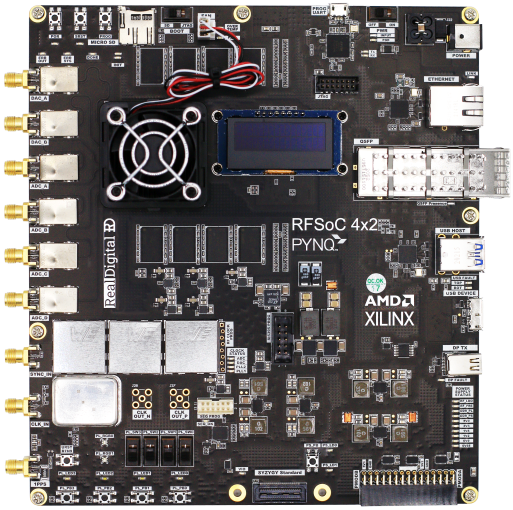
\includegraphics[width=0.6\textwidth]{Setup-software/figures/rfsoc4x2.png}
    \caption{Picture of a RFSoC4x2 board.}
    \label{fig:rfsoc4x2}
\end{figure}

The \RFSoC is much smaller than the \ZCU, while it is smaller, the \RFSoC is a FPGA of third generation, meaning it has much higher sampling frequencies.
Since there are just two DACs, this board can be used to control a single non-flux-tunable qubit. The connections will be:
\begin{itemize}
    \item \textbf{DAC 1:} drive line
    \item \textbf{DAC 2:} readout line
    \item \textbf{ADC 1:} feedback line (for readout)
    \item \textbf{ADC 2:} not active
    \item \textbf{ADC 3:} not active
    \item \textbf{ADC 4:} not active
\end{itemize}
As visible in \cref{fig:rfsoc4x2} \RFSoC has direct connections to SMA cables so it does not require any specific additional connector.
By \textit{not active} I mean that the firmware used never activates it; a different firmware potentially could.

On the other hand, the \ZCU board is a bit more complex. As is visible in \cref{fig:zcu111} there are no SMA connectors and an additional board is needed to convert from the black band connectors (the two band on the left in the figure) to SMAs.
\begin{figure}[ht]
    \centering
    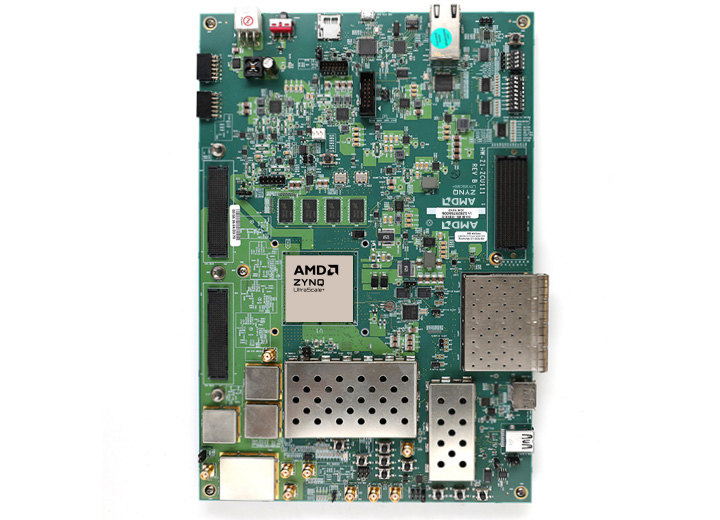
\includegraphics[width=\textwidth]{Setup-software/figures/zcu111.jpg}
    \caption{Picture of a ZCU111 board.}
    \label{fig:zcu111}
\end{figure}

Fortunately, with the \ZCU is sold by default a \textbf{XM500} board, shown in \cref{fig:xm500}.\\
Unfortunately, the \textbf{XM500} board is not just a convertor, but also adds some filtering and changes the output in non trivial ways.
\begin{figure}[ht]
    \centering
    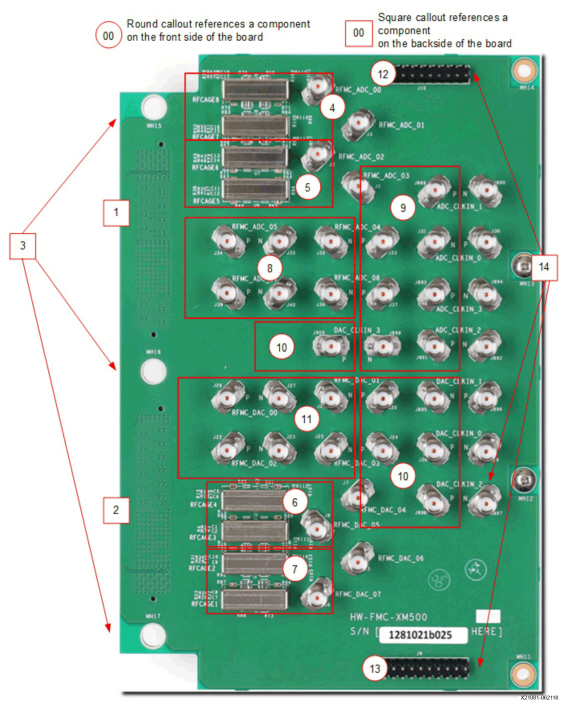
\includegraphics[width=0.65\textwidth]{Setup-software/figures/xm500.jpeg}
    \caption{Picture of a XM500 board.}
    \label{fig:xm500}
\end{figure}
In particular, the \textbf{XM500} has:
\begin{itemize}
    \item \textbf{external clock inputs/outputs:} not active;
    \item \textbf{4 single output DACs:} these are all active, but they have a balun filter added to it. That is a high-pass filter that removes DC components. So these cannot be used for DC flux control;
    \item \textbf{2 ADC:} active and also with baluns (but there are no downsides here);
    \item \textbf{3 differential output DACs:} these do not have baluns, so they can be used for flux lines, but require specific differential amplifiers to subtract the two outputs to convert them to a single SMA (also, the vast majority of differential amplifiers does not work for DC signals).
\end{itemize}

For the \ZCU, the \Qick project offers two different firmwares: one uses both ADCs, so can be used to control up to two flux-tunable qubits, the other uses a single ADC multiplexed.
The multiplex firmware is of particular interest and has been extensively used during the thesis.
Loading it, one of the DACs become capable of sending 4 different pulses at different frequencies but at the same time, while one of the ADC becomes capable of acquiring 4 different pulses (again at 4 different frequencies) at the same time.

This is one of the perks of using a re-configurable FPGA: since the ADCs and DACs are products of the FPGA logic is possible to reconfigure them so that a single ADC is actually composed of 4 with smaller bandwidth.\\
For this configuration, anyway, we used a standard upconversion system for the DAC so that, even with a smaller $f_s$, the output was in the first Nyquist zone (for power reasons).
\section{Developed Control Software}\label{sec:software}
My thesis work was included in the development of \Qibolab~\cite{Efthymiou_2023}, the instrument-related component of the \Qibo~\cite{qibo-website} framework.

\begin{figure}[ht]
    \makebox[\textwidth][c]{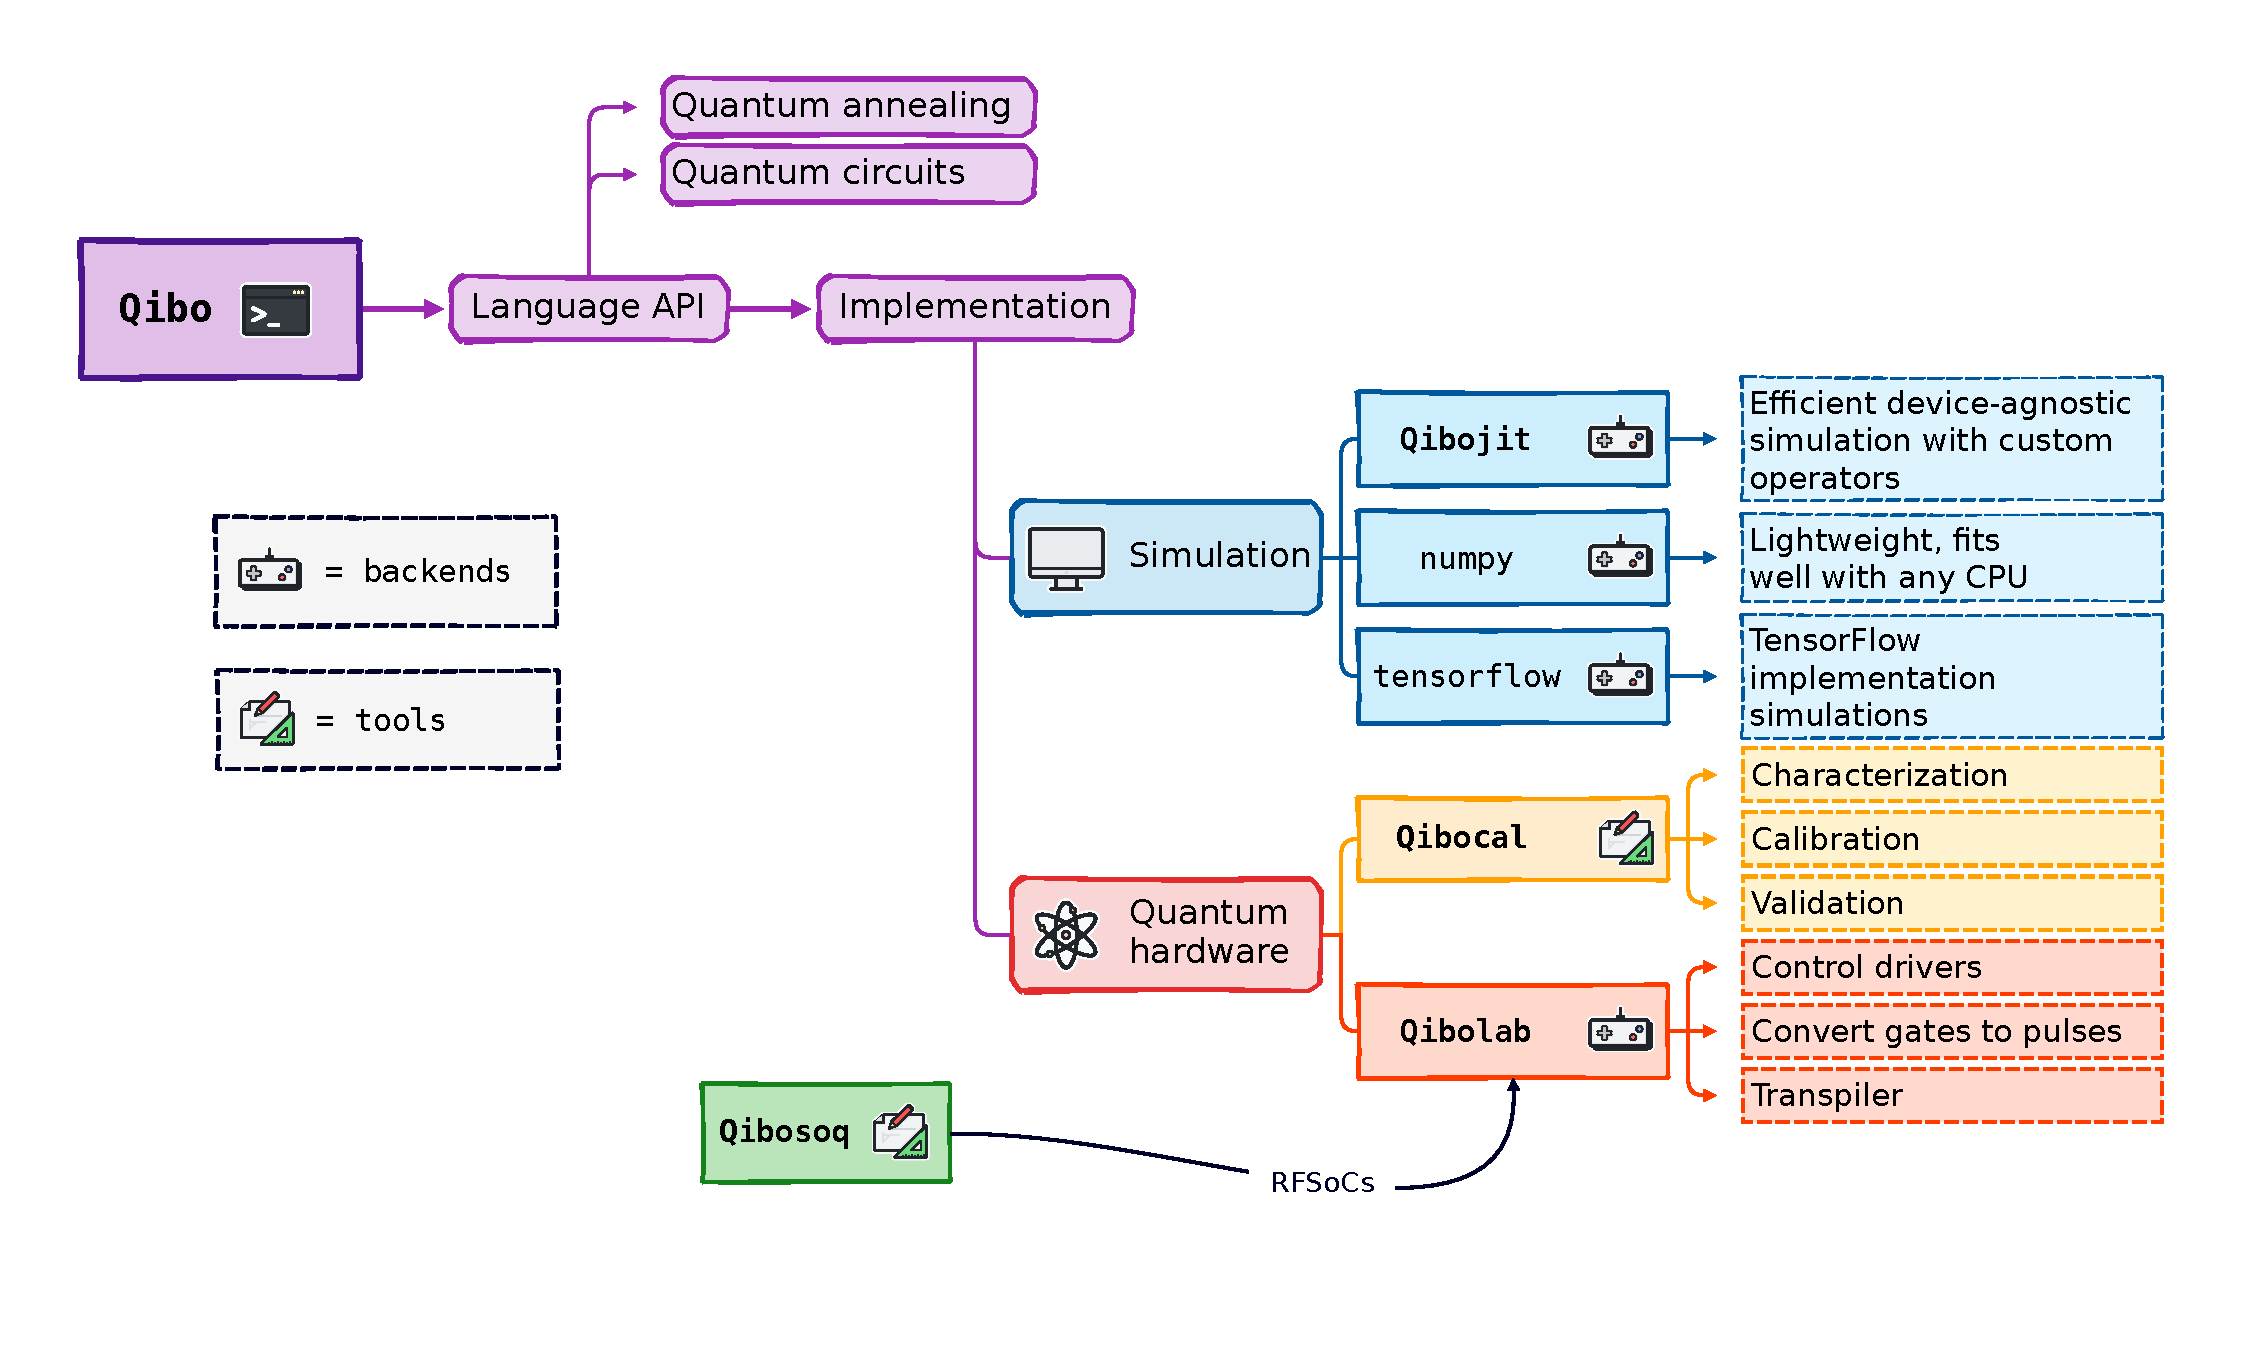
\includegraphics[width=1.3\textwidth]{Setup-software/figures/qibo_ecosystem.pdf}}
    \caption{Schematic overview of \Qibo software components.}
    \label{fig:qibo-ecosystem}
\end{figure}

\Qibo, schematically illustrated in \cref{fig:qibo-ecosystem}, is an open-source~\cite{qibo-github,qibolab-github,qibosoq-github} full stack application for quantum simulation that can be used to define and efficiently simulate circuits. 
It supports various backends for the execution of circuits: all of them are related to simulations, but one.

\Qibolab is the backend dedicated to hardware control and for deployment of circuits on real-quantum-hardware.
The idea behind \Qibolab is that of an hardware-agnostic software for hardware control that can be used in different laboratories without any development effort.\\
\Qibolab supports different control devices: in particular the systems of Quantum Machines, QBlox, Zurich-Instruments and, after my thesis, several RFSoC FPGAs.

In particular, I developed a two-side driver: composed of a client (the \Qibolab component) and a server called \Qibosoq.
The latter is a server that runs on the FPGA CPU present on the RFSoC boards and has the task of translating the programs received by \Qibolab (that are in the form of sequences of pulses) to a \Qick program.
\Qick contains both the firmware of the FPGAs and a low-level software to interact with the FPGA logic.

In this section I will give a general overview of the \Qibolab project, its components and abstraction levels and I will provide some details on the implementation of the RFSoC driver as well as of the \Qibosoq package. 

\subsection{Qibolab}

\Qibolab is the \Qibo backend dedicated to hardware execution.

Ideally, \Qibolab wants to be a universal control software for quantum computing, usable in the control of different qubit technologies by different electronics.
The philosophy that is guiding the development of this tool is the \textit{middleware} one, from RedHat.com:
\begin{quote}
    Middleware is software and cloud services that provide common services and capabilities to applications and help developers and operators build and deploy applications more efficiently. Middleware acts like the connective tissue between applications, data, and users.
\end{quote}

So that's the idea. In a moment in which, for quantum computing, no instrument is compatible with another one, where every technology and company implements a new programming language, where there is no convention between different constructors, \Qibolab wants to be the glue.

The key features of the API (Application Programming Interface, namely the software abstractions and functionalities), as it is now, are:
\begin{itemize}
    \item support for \Qibo circuits deployment on quantum hardware;
    \item support for different instruments for custom lab setups and easy integration of new drivers;
    \item support for different heterogeneous platforms (qubit systems);
    \item re-usability of calibration experiments via \Qibocal.
\end{itemize}

\Qibolab is a complex library and is currently composed of roughly $25000$ lines of Python code ($79000$ total lines including also documentation and tests), its main components are:

\begin{description}
    \item[Platform] this is the object that orchestrates different instruments in a laboratory, it describes a set of controlled qubits, controller device and any additional required device to coordinate;
    \item[Qubits] objects that contain characterization/calibration parameters, information about native calibrated gates and the connected channels;
    \item[Channels] physical wires in a laboratory that describe the setup and the connection among instruments and between the controller and the qubit;
    \item[Pulses] extensive API to work with pulses and pulse sequences. It includes support of various shapes;
    \item[Sweepers] these are objects crucial for experiments since they enable fast scans directly looping on FPGA logic;
    \item[Transpiler and Compiler] two components that, working together, are in charge of converting a circuit to a list of pulses (first as a circuit of native gates and then as a list of "native pulses");
    \item[Instruments] one  of the most important parts of \Qibolab, comprehensive support of different instruments under the same interface.
\end{description}

The main instruments, often called controllers, are shown in \cref{fig:qibolab_instruments}, while a list of supported features is available in \cref{tab:drivers-features}.

\begin{figure}[ht]
    \centering
    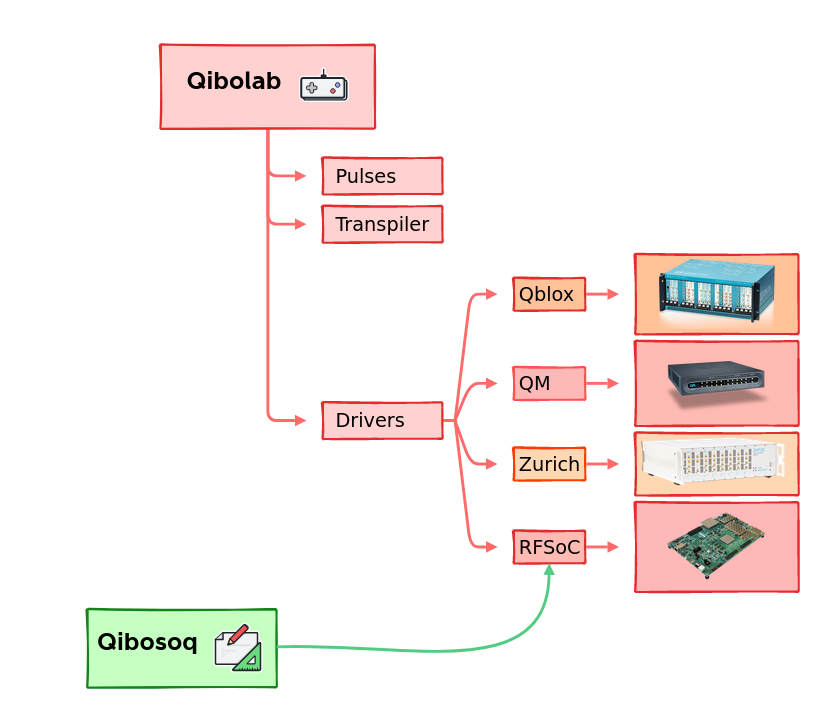
\includegraphics[width=0.8\textwidth]{Setup-software/figures/qibolab_instruments.png}
    \caption{Schematic overview of \Qibolab supported instruments.}
    \label{fig:qibolab_instruments}
\end{figure}

\begin{table}[ht]
\centering
	\begin{tabular}{lcccc}
  \hline \hline
		\textbf{Feature}              & \textbf{RFSoCs}    & \textbf{Qblox}    & \textbf{QM}        & \textbf{Zhinst}   \\ \hline
		Arbitrary pulse sequences     & \usym{1F5F8}  & \usym{1F5F8} & \usym{1F5F8}  & \usym{1F5F8} \\
		Arbitrary waveforms           & \usym{1F5F8}  & \usym{1F5F8} & \usym{1F5F8}  & ~\usym{1F5F8}\footnote{Sweeper capabilities may be reduced by using arbitrary pulses instead of driver defined ones.}      \\
		Multiplexed readout           & \usym{1F5F8}  & \usym{1F5F8} & \usym{1F5F8}  & \usym{1F5F8} \\
		Hardware classification       & \usym{2613}  & \usym{1F5F8} & \usym{1F5F8}  & \usym{1F5F8} \\
		Fast reset                    & \usym{1F4BB}   & \usym{1F4BB} & \usym{1F4BB}   & \usym{1F4BB}  \\
		Device simulation             & \usym{2613}  & \usym{2613} & \usym{1F5F8}  & \usym{1F4BB}  \\
		RTS frequency                 & ~\usym{1F5F8}\footnote{RTS on the frequency of readout pulses not supported.}    & \usym{1F5F8} & \usym{1F5F8}  & \usym{1F5F8}      \\
		RTS amplitude                 & \usym{1F5F8}  & \usym{1F5F8} & \usym{1F5F8}  & \usym{1F5F8} \\
		RTS duration                  & \usym{2613}  & \usym{1F5F8} & \usym{1F5F8}  & \usym{1F5F8} \\
		RTS start                     & \usym{1F5F8}  & \usym{1F5F8} & \usym{1F5F8}  & \usym{1F5F8} \\
		RTS relative phase            & \usym{1F5F8}  & \usym{1F5F8} & \usym{1F5F8}  & \usym{1F5F8} \\
		RTS 2D any combination        & \usym{1F5F8}  & \usym{1F5F8} & \usym{1F5F8}  & \usym{1F5F8} \\
		Sequence unrolling            & \usym{1F4BB}   & \usym{1F4BB} &\usym{1F4BB}  & \usym{1F4BB} \\
		Hardware averaging            & \usym{1F5F8}  & \usym{1F5F8} & \usym{1F5F8} & \usym{1F5F8} \\
		Singleshot (No Averaging)     & \usym{1F5F8}  & \usym{1F5F8} & \usym{1F5F8} & \usym{1F5F8} \\
		Integrated acquisition        & \usym{1F5F8}  & \usym{1F5F8} & \usym{1F5F8} & \usym{1F5F8} \\
		Classified acquisition        & \usym{1F5F8}  & \usym{1F5F8} & \usym{1F5F8}  & \usym{1F5F8} \\
		Raw waveform acquisition      & \usym{1F5F8}  & \usym{1F5F8} & \usym{1F5F8}  & \usym{1F5F8} \\
    \hline \hline
	\end{tabular}
	\caption[Supported features and limitations of \Qibolab \texttt{0.1.0}]{Features or limitations of the main drivers supported by \Qibolab \texttt{0.1.0}.
	The features denoted by `` \protect\usym{1F5F8} " are supported, `` \protect\usym{2613} "
  means not supported and `` \protect\usym{1F4BB} " under development.}
	\label{tab:drivers-features}
\end{table}

The following is a description of the features presented in \cref{tab:drivers-features}.
\begin{description}
    \item[Arbitrary pulse sequences] the capability of executing arbitrary pulse sequences defined in \Qibolab, which is a fundamental requirement of a driver. This feature is not related to the execution of pulses with arbitrary \textit{waveform shapes}.
    \item[Arbitrary waveforms] the capability of executing pulse waveforms of arbitrary shape. For drivers that do not support this feature, rectangular, Gaussian and Derivative Removal by Adiabatic Gate (DRAG~\cite{Gambetta2011}) waveforms can still be synthesized.
    \item[Multiplexed readout] allows playing and acquiring multiple multiplexed pulses through the same line. It is particularly useful for multi-qubit chips where the readout line is commonly shared among multiple qubits.
    \item[Hardware classification] the capability of doing single shot measurement classification \textit{during the execution} of a pulse sequence.
    \item[Fast reset] the capability of actively resetting the state of a qubit to zero after a measurement. This feature requires hardware classification and enables faster executions of repeated pulse sequences.
    \item[Device simulation] the possibility of simulating in advance the pulses to be executed, without directly using quantum hardware.
    \item[RTS frequency] RTS (\textit{Real Time Sweeper}) refers to the capability of executing a pulse sequence multiple times with different values of, in this case, the frequency of a pulse. This feature facilitates faster qubit characterization and experiments.
    \item[RTS amplitude] real-time sweeping of the amplitude of a pulse.
    \item[RTS duration] real-time sweeping of the duration of a pulse.
    \item[RTS start] real-time sweeping of the start time of a pulse.
    \item[RTS relative phase] real-time sweeping of the relative phase of a pulse.
    \item[RTS 2D] the capability of combining two RTS scans on different parameters.
    \item[Sequence unrolling] the capability of converting a sequence repeated multiple times, in a minor number of longer sequences that each contains multiple measurements, in order to decrease the overall time spent on pulse compilation and communication to the devices.
    \item[Hardware averaging] the capability of repeating the same experiment multiple times and obtain, directly from the device, averaged results.
    \item[Singleshot (No Averaging)] the capability of obtaining from the devices all the non-averaged results.
    \item[Integrated acquisition] the capability of acquiring complex signals~\cite{Naidu2003} with "in-phase" and "quadrature" (IQ) components demodulated and integrated for the measuring time.
    \item[Classified acquisition] the capability of performing 0-1 state classification after the integrated acquisition.
    \item[Raw waveform acquisition] the capability of acquiring non-integrated IQ waveform values.
\end{description}

\Qibolab was also object of a recent publication, in which the contribution of the work related to this thesis was not indifferent: CITE.


\subsection{Qibosoq}

A large part of my work for this thesis focused on the development of the required software to integrate RFSoCs into the \Qibo framework through \Qibolab driver.
To do so, it was needed to build a comprehensive library that bridged the differences between \Qibolab and \Qick (that has the task of controlling the FPGA logic).
This were the premises for \Qibosoq.

\Qibosoq is a an open-source server-side software package designed for RFSoC for executing arbitrary pulse sequences on self-hosted quantum processing units.

Its layout is essentially divided in three main elements:
\begin{description}
    \item[Client:] the user of the RFSoC, connected remotely via any network connection;
    \item[Server:] the always-listening server running directly on the board. It takes care of receiving commands from the client and to execute the experiments;
    \item[Language API:] a set of objects that define a common language between client and server.
\end{description}

The server role is to take commands and programs defined in the \Qibosoq language and compile them as an executable that can be run by the \Qick tProcessor: a timed processor on the FPGA logic that takes care of orchestrating firing pulses.

\Qibosoq exposes various tools and abstractions to the user: the \textbf{programs}, representing \Qick programs, and eventually taking care of the experiment compilation into the tProcessor language, the \textbf{components}, high-level structures used in the \textit{programs} construction, the \textbf{server} implementation, and \textbf{client} utilities, to manage the communication.

The \textbf{programs} bridge the gap between the high-level interfaces (components) and the low-level execution on quantum hardware.
Eventually, only two distinct programs are directly used, but the full hierarchy also includes intermediate abstractions.
Considering all layers, the defined \textbf{programs} are:
\begin{itemize}
    \item the abstract \textbf{base} program, that contains functions shared among all possible experiments and executions. It serves as the foundation for all the other \Qibosoq programs;
    \item the abstract \textbf{flux} program, that collects the additional elements required for controlling flux-tunable qubits. In addition to the functionalities defined in \textbf{base}, it includes support for bias voltages and fast DC (direct current) pulses.
    \item the \textbf{sequences} and \textbf{sweepers} programs, that contain the different elements used, respectively, in the execution of fixed parameters pulse sequences and real-time sweeps. They inherit all the functionalities defined in \textbf{base} and \textbf{flux}.
\end{itemize}

The \textbf{components} play the crucial role of establishing a common language for communication, easing the implementation of a \Qibosoq client in \Qibolab or by other parties.
The main elements defined within the \textbf{components} submodule include:
\begin{itemize}
    \item the \textbf{Config} object that contains essential general information required for execution on hardware, such as the number of repetitions for the experiment and the waiting time between repetitions;
    \item the \textbf{Pulse} base object that serves as the foundation for different implemented pulse shapes. Rectangular, Gaussian and DRAG~\cite{Gambetta2011} pulses are natively supported, as well as custom waveform shapes defined by their ''in-phase`` and ''quadrature`` (IQ)~\cite{Franks1969,Naidu2003} values;
    \item the \textbf{Qubit} object that describes a qubit and holds information about any necessary bias required for its operation~\cite{Hutchings2017};
    \item the \textbf{Sweeper} and \textbf{Parameter} objects that are used to describe real-time on-hardware scans.
\end{itemize}

\begin{table}[ht]
\centering
	\begin{tabular}{lccc}
  \hline \hline
		\textbf{Feature}  & \textbf{Qick} & \textbf{Qibolab} & \textbf{Qibosoq} \\ \hline
		Arbitrary pulse sequences     & \usym{1F5F8}  & \usym{1F5F8} & \usym{1F5F8}\\
		Arbitrary waveforms           & \usym{1F5F8}  & \usym{1F5F8} & \usym{1F5F8} \\
		Multiplex readout             & \usym{1F5F8}\footnote{Special firmware available from \Qick under request}  & \usym{1F5F8} & \usym{1F5F8} \\
		Feedback                      & \usym{1F5F8}  & \usym{1F5F8} & \usym{26ED} \\
		RTS frequency drive           & \usym{1F5F8} & \usym{1F5F8} & \usym{1F5F8}      \\
		RTS frequency readout         & \usym{2613}  & \usym{1F5F8} & \usym{2613}     \\
		RTS amplitude                 & \usym{1F5F8}  & \usym{1F5F8} & \usym{1F5F8} \\
		RTS duration                  & \usym{2613}  & \usym{1F5F8} & \usym{2613}  \\
		RTS start                     & \usym{1F5F8}  & \usym{1F5F8} & \usym{1F5F8}   \\
		RTS relative phase            & \usym{1F5F8}  & \usym{1F5F8} & \usym{1F5F8}   \\
		RTS N-Dimensional             & \usym{1F5F8}  & \usym{1F5F8} & \usym{1F5F8}   \\
		Hardware averaging            & \usym{1F5F8}  & \usym{1F5F8} & \usym{1F5F8}  \\
		Singleshot (No Averaging)     & \usym{1F5F8}  & \usym{1F5F8} & \usym{1F5F8}  \\
		Integrated acquisition        & \usym{1F5F8}  & \usym{1F5F8} & \usym{1F5F8}  \\
		Raw waveform acquisition      & \usym{1F5F8}  & \usym{1F5F8} & \usym{1F5F8}   \\
    \hline \hline
	\end{tabular}
	\caption[Comparison of the supported features of \Qibolab, \Qick and \Qibosoq]{Main features and limitations of \Qick, \Qibosoq and \Qibolab compared.
	The features denoted by `` \protect\usym{1F5F8} '' are supported, `` \protect\usym{2613} ''
    means not supported and `` \protect\usym{26ED} '' under development.}
	\label{tab:supported-features_qibosoq}
\end{table}


The last two fundamental elements are the \textbf{client} and the \textbf{server}.
The \textbf{client} is composed of a set of tools used to connect to the server, convert components into a serialized form, and send them following the \Qibosoq communication protocol.
The \textbf{server} implements the on-board server, continuously listening for connections, and executing received instructions by initializing and running the required programs on the quantum hardware.

In analogy of what was presented for \Qibolab, in \cref{tab:supported-features_qibosoq} are presented the main features supported by \Qibosoq in comparison with what is supported by \Qick and \Qibolab.


\Qibosoq was developed for this thesis and is now a small complete library of $2500$ lines of python code (total of $8000$ lines) has been recently object to arXiv publication:~\cite{qibosoq_paper}.


\chapter{Single qubit characterization and calibration}


The focus of this thesis is the characterization and calibration of superconducting qubits~\cite{Roth2021}.

The two words, \textit{characterization} and \textit{calibration}, are often used as synonyms, but it is useful to introduce a difference:
\begin{itemize}
    \item characterization means finding the values of \textit{intrinsic} properties of the qubit (for example its resonance frequency, its $T_1$...);
    \item calibration means finding the optimal parameters to \textit{control} the qubit.
\end{itemize}

The following parameters are the main ones to be obtained in characterization experiments:
\begin{description}
    \item[Qubit resonance frequency] The qubit resonance frequency refers to the specific frequency at which a qubit undergoes a transition between its first two energy levels. This parameter that determines the operational frequency of the qubit.
    \item[Resonator resonance frequency] The resonator resonance frequency is the natural frequency at which a resonator oscillates. This frequency is dependent on the physical characteristics of the resonator and is essential for readout operations.
    \item[Q factors] Quality factors measure the damping of oscillations in a resonant system. A high Q factor indicates minimal damping and high energy efficiency, while a low Q factor indicates significant damping. In the context of quantum systems, a high Q factor is desirable for maintaining coherence and prolonging the lifetime of quantum states. It is defined as $Q = \frac{f_r}{\Delta f_r}$
    \item[Coupling $g$ ] The coupling parameter $g$ represents the strength of the interaction between two quantum components, such as a qubit and a resonator. It determines the rate at which energy is exchanged between the components.
    \item[Dispersive shift] The dispersive shift is a phenomenon in quantum systems where changes in the energy levels of a qubit are observed due to its interaction with a resonator. This shift depends on the state of the resonator and can be used for qubit readout and manipulation.
    \item[Anharmonicity] Anharmonicity refers to the nonlinearity of the energy levels of a quantum system and signifies that the energy difference between different quantum states is not strictly equal.
    \item[Relaxation time $T_1$] The relaxation time $T_1$ characterizes the time it takes for a qubit to return to its ground state from an excited state. It quantifies the qubit's tendency to lose energy and coherence, often due to interactions with the environment.
    \item[Dephasing time $T_2$] The dephasing time $T_2$ represents the duration during which a qubit can maintain coherence without undergoing energy-changing transitions. It measures the qubit's resilience against fluctuations and noise in its environment.
\end{description}

As we can see, characterization parameters are intrinsic properties of the qubit system and come mostly from fabrication.\\
On the other hand, we have calibration experiments that analyze optimal control parameters:

\begin{description}
    \item[Drive frequency] The optimal frequency of the pulses required to change the state of the qubit.
    \item[Drive amplitude] The optimal amplitude of the pulses used to change the rotate the state of the qubit on the Bloch sphere, as well as the mapping between amplitudes and rotated degrees.
    \item[Drive duration \& shape] The optimal duration and shape of the control pulses to change the qubit state as required and minimizing leakage to higher excited states.
    \item[Assignment fidelity] Parameters to classify the states, zero and one, from IQ values as well with assignment fidelities.
    \item[Time of flight] time required for a signal to travel from the RFSoC to the qubit and back, required for pulse control and readout.
    \item[Readout frequency] The optimal frequency of the pulses required to read the state of the qubit.
    \item[Readout amplitude] The optimal amplitude of the pulses required to read the state of the qubit
    \item[Readout duration \& shape] The optimal duration and shape of the pulses required to optimize the read-out the state of the qubit
    \item[Gate fidelity] The accuracy relative to specific operation that differ from an exact matrix, by some measurable factor.
\end{description}

%In \cref{tab:calibration_parameters} some of the main parameters of calibration are listed.

%In \cref{tab:characterization_parameters,tab:calibration_parameters} are listed the main parameters to be obtained with characterization and calibration experiments.
%Although some concept may be unfamiliar, this should help distinguish the two processes, while more details will be given in the next sections.
%
%\begin{table}[ht]
%    \centering
%    \begin{tabular}{l|l}
%        Qubit resonance frequency &  Resonator resonance frequency\\
%        Q factors & Coupling $g$ \\
%        Dispersive shift & Anharmonicity \\
%        $T_1$ & $T_2$ \\
%    \end{tabular}
%    \caption{Main parameters to be obtained with characterization.}
%    \label{tab:characterization_parameters}
%\end{table}
%
%\begin{table}[ht]
%    \centering
%    \begin{tabular}{l|l}
%        Drive frequency &  Readout frequency\\
%        Drive amplitude & Readout amplitude \\
%        Drive duration \& shape & Readout duration \& shape \\
%        Assignment fidelity & Gate fidelity \\
%        Time of flight & \\
%    \end{tabular}
%    \caption{Main parameters to be obtained with calibration.}
%    \label{tab:calibration_parameters}
%\end{table}

The difference is often minimal and many experiments fall in both categories at the same time, but nevertheless the difference is substantial.
In particular, the objective of an experimenter may be just in characterization, so with no interest in optimizing the control of the qubit, or just in calibration, with only interest in reaching good control without interest in knowing parameters such as quality factors or coupling values.

In this chapter (and this thesis), I will try to give a description and some examples for all the most important experiments in single qubit characterization and calibration.
Note that the list hereby provided is not exhaustive at all and, in particular for calibration, the possible experiments are almost unlimited.

The main sources for this chapter, that are maybe more precise and advanced then this thesis are \cite{Gao2021, Kim2023, Naghiloo2019, Zijun2018}.\\
This chapter, on the other hand, tries to present the experiments in the clearest possible way, so that they can easily reproduced.
For every experiment, ideal and real-case plots are provided so that the reader can have a better grasp of the differences between the ideal situation and the reality.\\
Moreover, at the end of every experiment a short recap will be provided, in the form of a blue color box.

In the case of flux-tunable devices, some more experiments are needed: these experiments will always have names starting with "Flux ..." and will be differentiated by the others also by the use of a red recap box.
These experiment can/have to be avoided in the case of non-flux-tunable qubit characterization.

\begin{figure}[htbp]
    \centering
    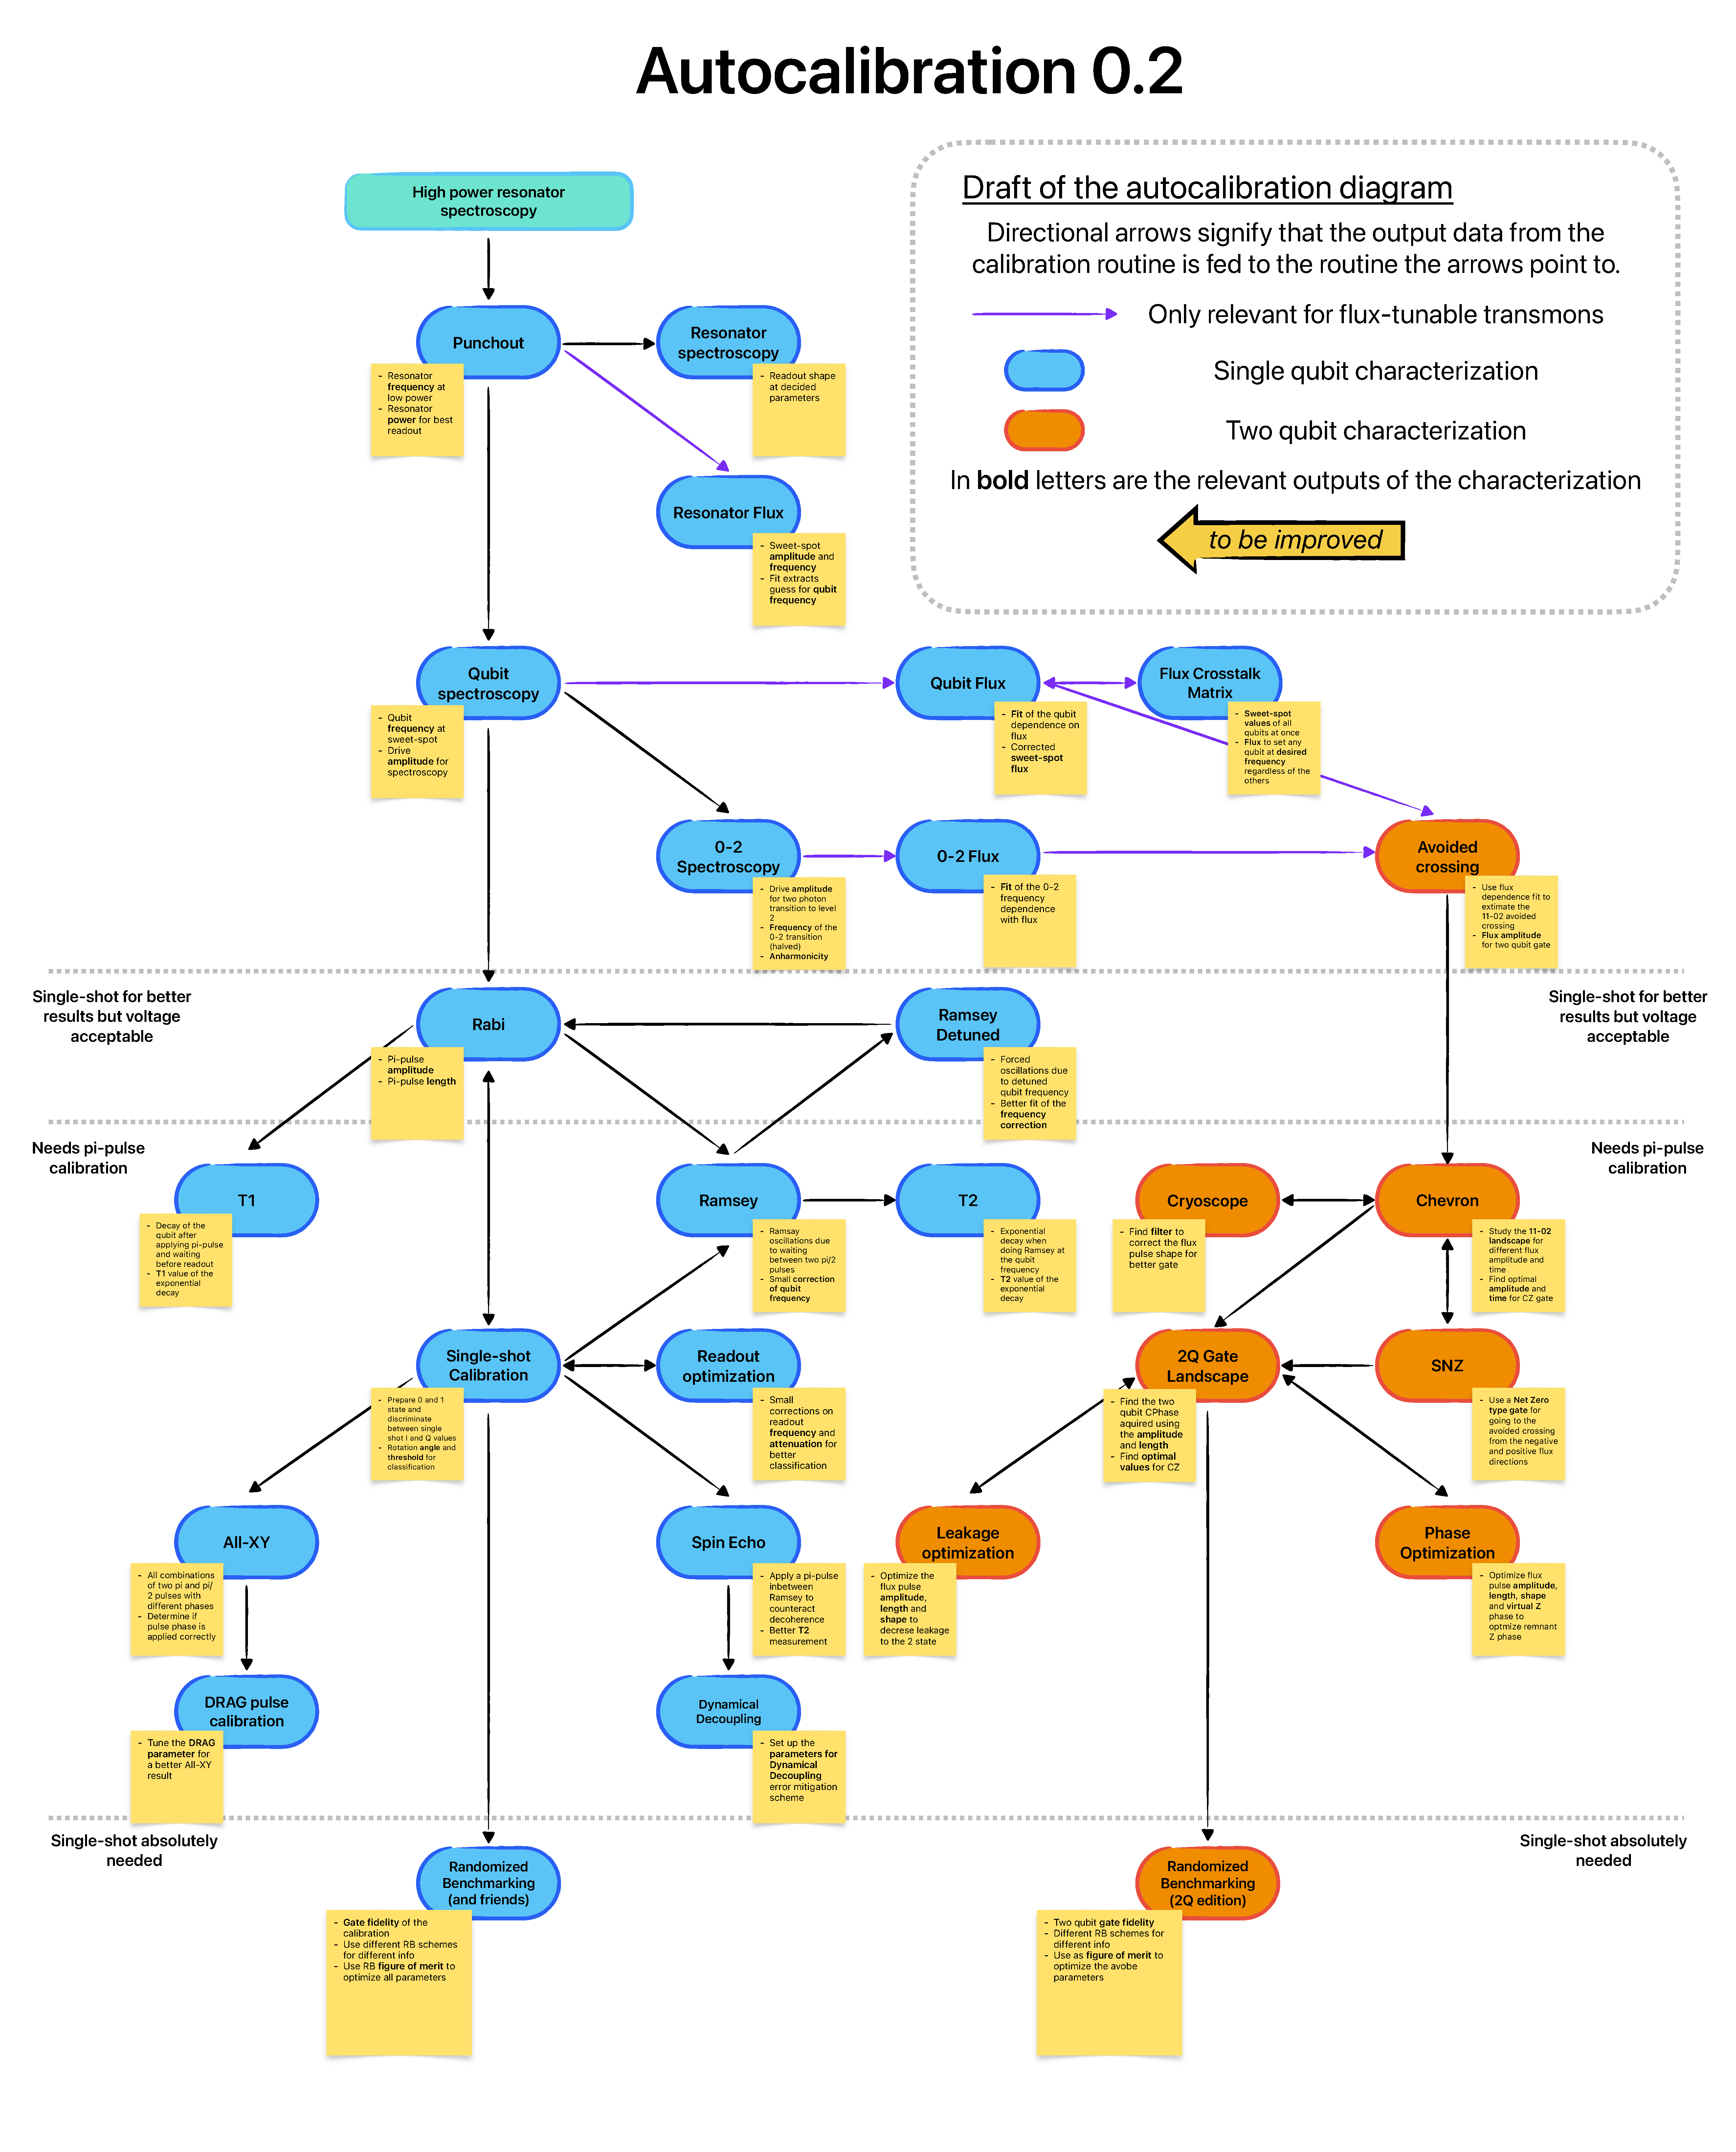
\includegraphics[width=\textwidth]{characterization/figures/Autocalibration 0.2.pdf}
    \caption{Scheme of the characterization and calibration experiments as presented for \Qibocal auto-calibration module.}
    \label{fig:scheme_experiments}
\end{figure}

In \cref{fig:scheme_experiments}, an outline of the main experiments described in this chapter is presented as per the proposal for the auto-calibration module of \Qibocal. Several experiments are mentioned in the scheme and not yet available, so not described in this thesis.

Note that, while they are in order of priority (top to bottom), characterization and calibration \textbf{is not} a sequential process.
It will happen many times, as an experimenter, to go back in the experiments tree and repeat some procedure, to better optimize some parameters.\\
The burden of understanding when to repeat an experiment is necessarily left to the reader/experimenter and the apparent sequentiality of this chapter is just a matter of simplicity.

\vspace{1cm}

\textbf{A note:} the majority of the plots presented in this chapter are produced by \Qibocal and shown here complete of a left amplitude plot and a right phase plot.
Our discussion will always focus only on the amplitude plot for simplicity, but it has to be clear that the majority of information can also be extracted from the phase plot.
In the end, there is direct amplitude measured, but always two I-Q values from which we can compute amplitudes and phases.\label{chap:char}

\newpage
\routine{Time of flight measurement}{time_of_flight}
\routine{Resonator spectroscopy (bare frequency)}{resonator_spectroscopy}
\routine{Resonator punchout}{punchout}
\routine{Flux resonator spectroscopy}{resonator_spectroscopy_flux}
\routine{Qubit spectroscopy}{qubit_spectroscopy}
\routine{Flux Qubit Spectroscopy}{qubit_spectroscopy_flux}
\routine{Rabi oscillation}{rabi_oscillations}
\routine{Ramsey experiment}{ramsey}
\routine{Flipping}{flipping}
\routine{T1 measurement}{t1_measurement}
\routine{Hahn’s spin echo (T2)}{t2_spin_echo}
\routine{Single-shot classification}{single_shot_classification}
\routine{Readout optimization}{readout_optimization}
\routine{AllXY}{allxy}
\routine{DRAG tuning (pulse shape)}{pulse_shape}
\routine{Randomize benchmarking}{rb}

\newpage

\routine{Other possible calibration experiments}{other_possible}




% two qubit gates things
\chapter{Two-qubits characterization and calibration}

After the last chapter, and with some more work and fine tuning, the experimenter should be able to reach a proper single qubit calibration.
However, to execute "useful" circuits, the capability of entangling multiple qubits and executing gates between them is critical.
Indeed, the real difference between classical and quantum computations \textit{is} the entanglement effect: from a probability point of view, all the results that we obtained are still compatible with classical theories (or hidden-variables theories) and we didn't yet encounter any real proof of quantum probability.

In this section, we will learn the principles of two-qubits gates and how to perform a basic calibration of those.
%The calibration presented here will be used in XXX to perform a Bell experiment and proof that this is indeed a quantum world.

There are two main two-qubits gates that can be implemented: CZ and iSWAP.
The calibration is more or less the same and the complexity to achieve them does not differ. 
I will focus on the iSWAP gate since I found better literature about it, but everything can be easily transposed for the CZ~\cite{Krantz2016, DiCarlo2009, McKay2017}.


The interaction of two qubits is done via a coupling capacity that produces an interaction term of:
\begin{equation}
    H_{qq} = g \sigma_{y1} \otimes \sigma_{y2}
\end{equation}
This Hamiltonian can be decomposed in $\sigma^\pm$ (ladder operators) and, dropping the fast rotating terms, we can arrive at:
\begin{equation}
    H_{qq} = g (e^{\delta \omega_{12}t}\sigma^+ \sigma^- + e^{-\delta \omega_{12}t}\sigma^- \sigma^+)
\end{equation}
where we have $\delta \omega_{12}= \omega_{q1} - \omega_{q2}$.

The last equation is not particularly clear and easy to understand, but this all changes when the two qubits share the same frequency:
\begin{equation}
    H_{qq}=g(\sigma^+\sigma^- + \sigma^-\sigma^+) = \frac{g}{2}(\sigma_x \sigma_x + \sigma_y \sigma_y)
\end{equation}
And this equation, when applied as a time evolution, produces an iSWAP gate.

The iSWAP gate can be written in the canonical basis as:
\begin{equation}
    iSWAP = 
    \begin{pmatrix}
        1 & 0 & 0 & 0 \\
        0 & 0 & -i & 0 \\
        0 & -i & 0 & 0 \\
        0 & 0 & 0 & 1
    \end{pmatrix}
\end{equation}
while the time evolution of $H_{qq}$ is:
\begin{equation}\label{eq:iswap_oscillations}
    U_{qq}(t) = e^{-i\frac{g}{2}(\sigma_x \sigma_x + \sigma_y \sigma_y)t}= 
    \begin{pmatrix}
        1 & 0 & 0 & 0 \\
        0 & \cos(gt) & -i\sin(gt) & 0 \\
        0 & -i\sin(gt) & \cos(gt) & 0 \\
        0 & 0 & 0 & 1
    \end{pmatrix}
\end{equation}
with exact equality for $T=\frac{\pi}{2g}$.

So, what we have just demonstrated can be summarized in saying that the iSWAP can be implemented simply by activating the two-qubits interaction for a fixed time.


\section{Avoided crossings}

The first step required to reach two-qubits gates is the avoided crossing experiment~\cite{Silveri2015, Sun2020}.
The objective here is to find, approximately, the flux and frequency where the interaction will happen.

In particular, since we are considering the iSWAP, we want to find the point in the flux-frequency space, where we can have a jump of states between $\ket{01}$ and $\ket{10}$.

We are considering to have two flux-controllable qubits already calibrated (at the single qubit level) so we are supposing to have already studied the flux dependency of those, but let's repeat some information.
Both qubits have a dependency between frequency and the flux passing through their SQUID.
They are characterized by a certain sweetspot, namely a certain flux value that moves the qubit to a frequency that is the maximum frequency reachable.
The application of less or more flux will reduce the frequency of the qubits.

Note that we now want to control both qubits at the same time and a flux applied at one will probably change also the other qubit. It's critical to take this in consideration in the research for the sweetspots.

Anyway, considering one qubit (A) at the sweetspot and the second qubit (B), that has a higher frequency at the sweetspot, swept in bias, we can obtain a plot similar to the one in \cref{fig:crossings}.

\begin{figure}[ht]
    \centering
    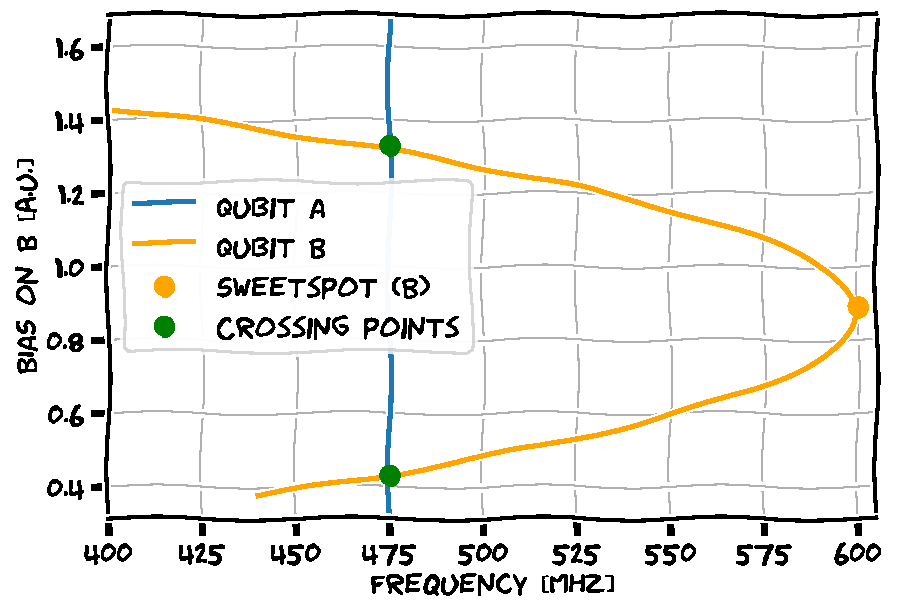
\includegraphics[width=8cm]{Two-qubits calibration/Figures/crossings.pdf}
    \caption{Possible behaviour of two qubits flux dependence.}
    \label{fig:crossings}
\end{figure}

Note that in \cref{fig:crossings} the lines are the ones drawn by the peaks in qubit spectroscopies that describes the transition $\ket 0 \leftrightarrow \ket 1$.

Note also that, if we define the two-qubits state as $\ket A \otimes \ket B = \ket{AB}$, we can identify the orange curve in the plot as the one of the $\ket{00} \leftrightarrow \ket{01}$ transition and the blue one as the $\ket{00} \leftrightarrow \ket{10}$ transition.
So at the green points we have precisely the condition required for the iSWAP and, to reach it, it seems that is just needed to apply two contemporary flux pulses at two qubits (with an amplitude computed from the distance from the sweetspot).

What actually is happening at the crossing points however, is an hybridization of the two states that can be solved analytically or just seen directly by zooming in the plot presented. 
See for example \cref{fig:avoided_crossing} (note that the axes are swapped).
\begin{figure}[ht]
    \centering
    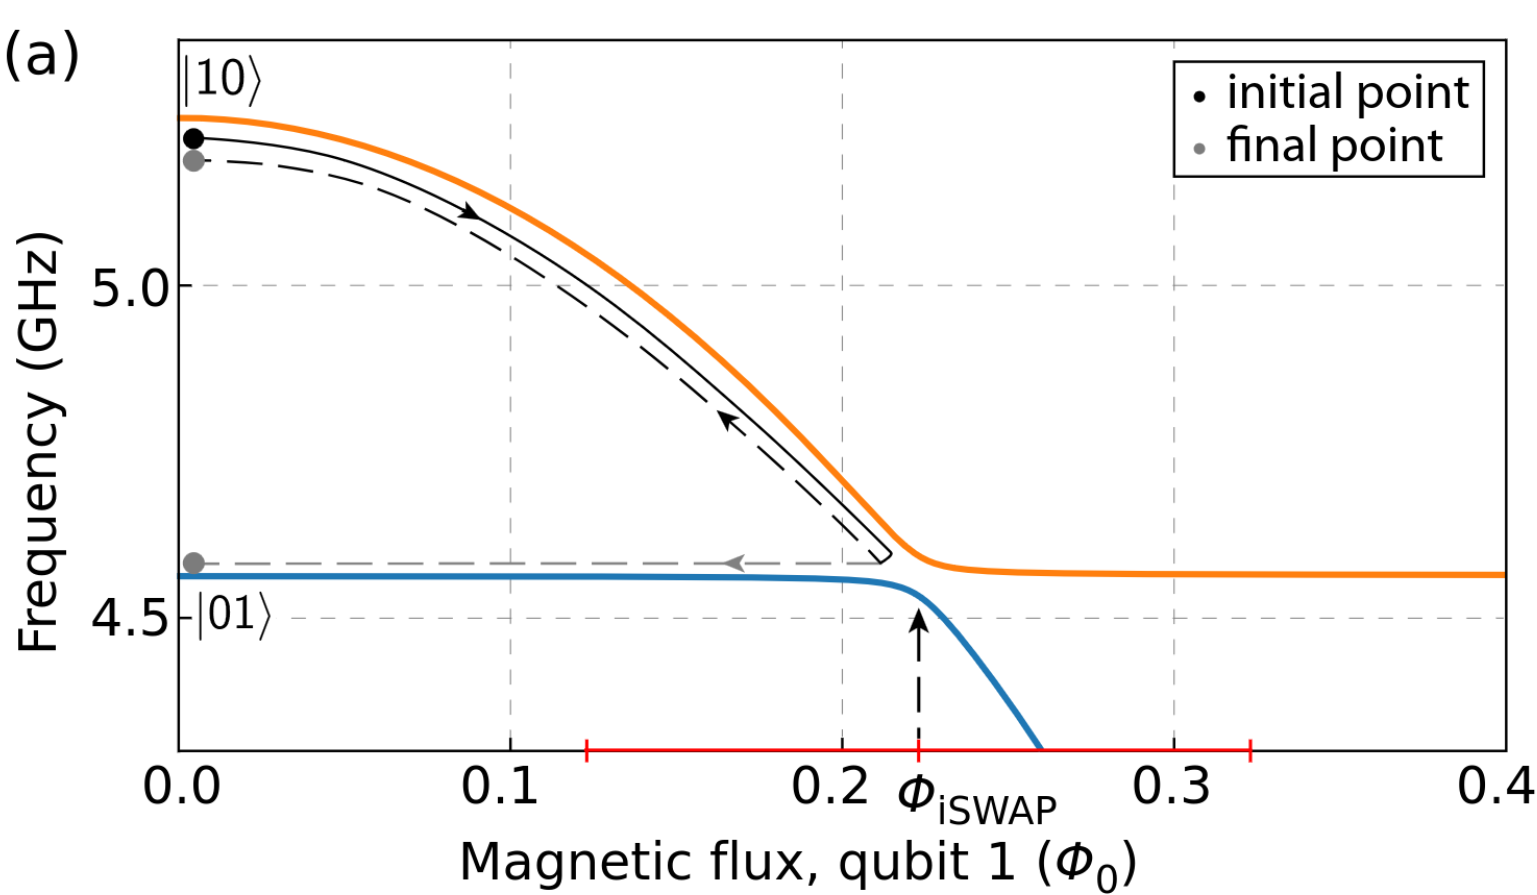
\includegraphics[width=8cm]{Two-qubits calibration/Figures/avoided_crossing.png}
    \caption{Avoided crossing.}
    \label{fig:avoided_crossing}
\end{figure}

In \cref{fig:avoided_crossing} it's defined also an initial and final state, that will be used for the iSWAP.

Finding the avoided crossings is the first step for two-qubits gates characterization.
After that, we know how much flux is needed to move the higher frequency qubit to the interaction point and we have proved (through avoided crossing) that an interaction is indeed present (but we still need to calibrate it).

Note that there are always two interaction points, but this are usually at different flux absolute values, so it's preferred to use the lower one (although the interaction would happen equally.

Note also that we now saw the avoided crossings for the iSWAP, but for the CZ the experiment is similar.
For the CZ we look for the interaction $\ket{02} \leftrightarrow \ket {20}$.
To see the second level transition frequency, it is sufficient to perform a qubit spectroscopy with more amplitude so that, just before the $\ket 0 \leftrightarrow \ket 1$ transition peak, also the $\frac{\ket 0 \leftrightarrow \ket 2}{2}$ can appear (divided by two because usually two combined photons can give those high energies).

A larger scan in frequencies can give us \cref{fig:avoided_crossing2}.
\begin{figure}[ht]
    \centering
    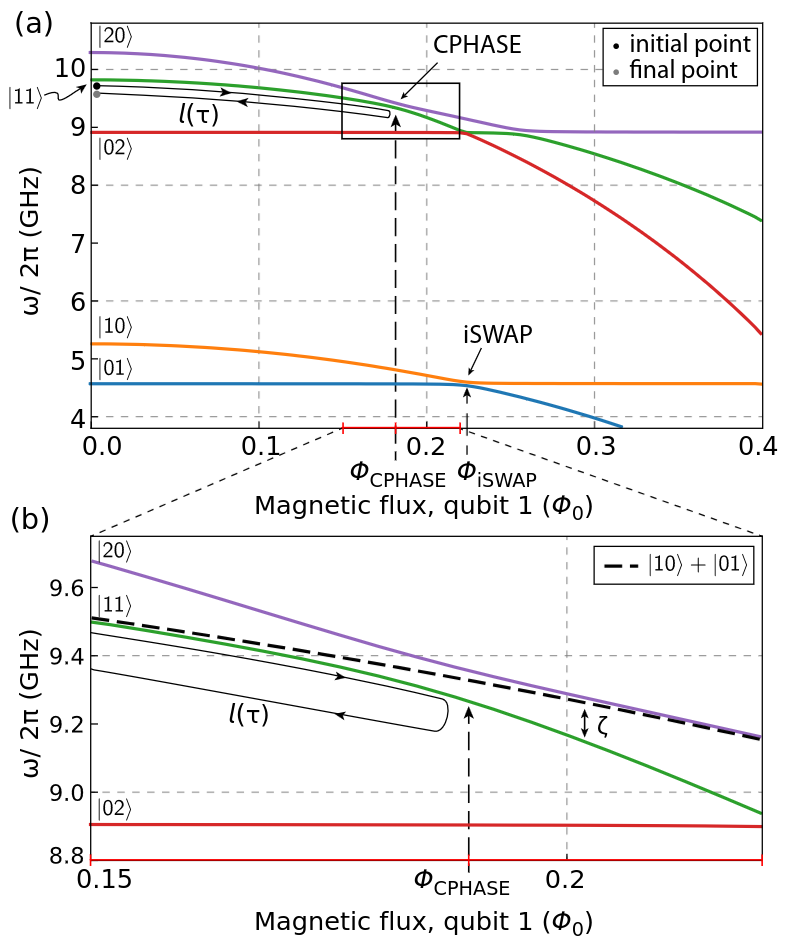
\includegraphics[width=8cm]{Two-qubits calibration/Figures/crossing_cz_iswap.png}
    \caption{Avoided crossing for CZ and iSWAP.}
    \label{fig:avoided_crossing2}
\end{figure}

In \cref{fig:crossings_large} are shown the results of a scan large both in flux and frequency.
The 4 horizontal lines are a low resolution visualization of the 4 avoided crossings (2 for CZ and 2 for iSWAP) with the inner two being the ones for CZ and the outer two of iSWAP.

\begin{figure}[ht]
    \centering
    \makebox[\textwidth][c]{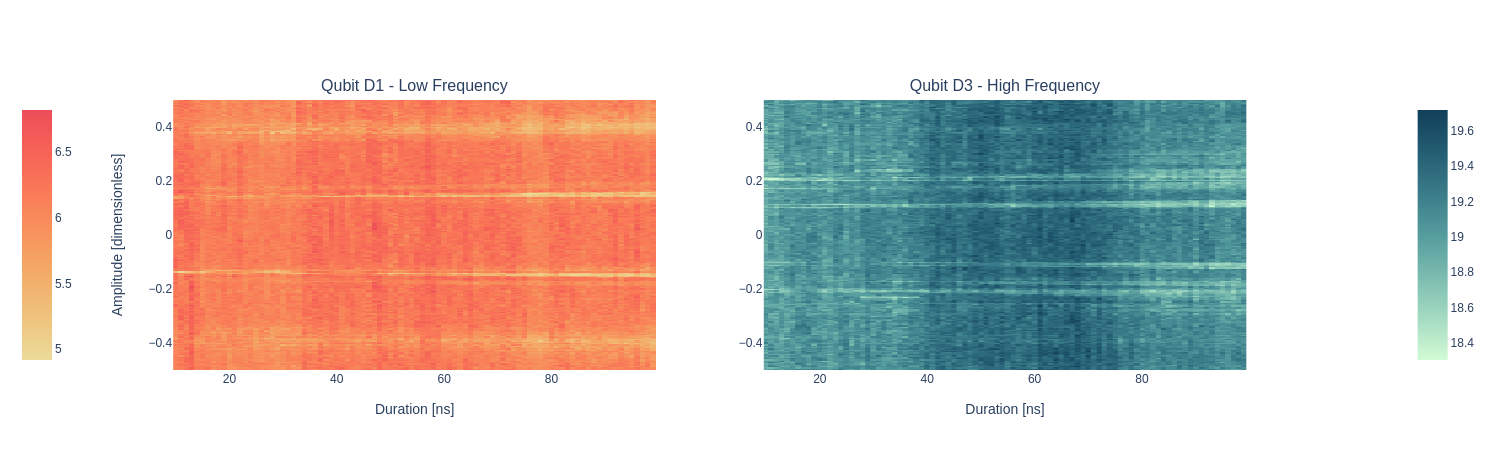
\includegraphics[width=1.3\textwidth]{Two-qubits calibration/Figures/large_chevron.png}}
    \caption{Large scan where all the 4 interaction biases are visible.}
    \label{fig:crossings_large}
\end{figure}

In \cref{fig:avoided_crossing_qblox} a zoom in on one of the iSWAP crossing points show the states hybridization and the avoided crossing phenomenon.

\begin{figure}[htbp]
    \centering
    \makebox[\textwidth][c]{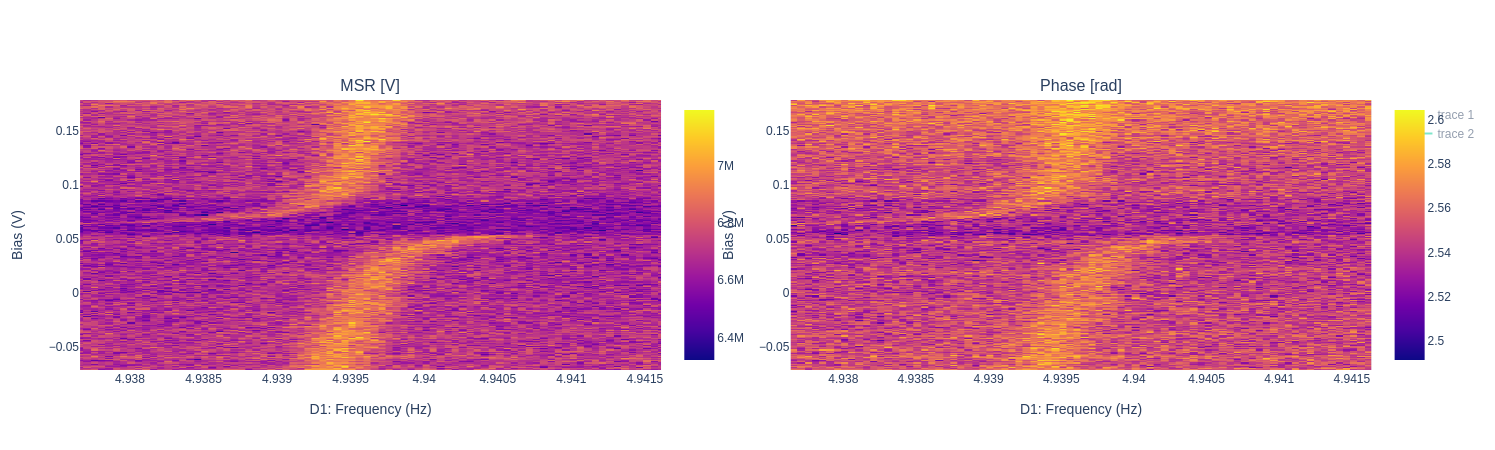
\includegraphics[width=1.3\textwidth]{Two-qubits calibration/Figures/my_avoided_crossing.png}}
    \caption{Zoom in on an avoided crossing (iSWAP). The bias is applied only to the high frequency qubit, while the lower is left at the sweetspot. Measuring the low-frequency qubit gives the avoided crossing.}
    \label{fig:avoided_crossing_qblox}
\end{figure}







\section{Chevron plot}

Now that we found an estimation of the interaction point, it's time to calibrate the gate~\cite{Gu2021}.

First we look back at \cref{fig:avoided_crossing} that was also showing the evolution of a state starting in $\ket{10}$.
Indeed if we prepare a state $\ket{10}$, using an already calibrated \pipulse on the first qubit, we can follow it up with a second pulse that moves the state along the orange curve.
This second pulse will be applied to qubit B and sent through the flux line on the qubit.
Ideally, there is no movement along the line, but only jumps: in the sense that, if we want to send a certain flux, we would like to not have any transient.
Because of this the flux pulse is initially defined as a rectangular pulse.

Let's try to understand the arrows drawn in \cref{fig:avoided_crossing}.
If we send a flux pulse with a flux of $0.1$ (considering the numbers in the plot) this will not be enough to reach the interaction point and, after the flux pulse in ended, measuring the two qubits will show that we still have a $\ket{10}$ state.
The same thing happen, more or less, if more flux than needed in sent.

If the flux value is correct, Rabi-like oscillations are produced between the two states as indicated in \cref{eq:iswap_oscillations}.
Actually, even at wrong fluxes we still achieve some Rabi-like oscillations, but with lower amplitude, higher frequencies, and lots of leakage to higher levels.

What we want to calibrate then, is the exact value of the flux needed for the two-qubit gate and the time $T$ to achieve the gate.
We perform an experiment with the following pulse sequence:
\begin{itemize}
    \item a first \pipulse is sent to qubit A (lower frequency);
    \item afterwards, a flux pulse in sent to qubit B (higher frequency);
    \item afterwards, a measurement is performed on both qubits;
    \item the experiment is repeated for various biases (around the expected crossing point) and various lengths.
\end{itemize}

The results of this experiment are plotted in a 3D graph with pulse-flux Vs pulse-length Vs $P_{01}$.
The z axis can actually represents different parameters: in particular probabilities regarding single qubit measurements (both for qubit A and B) or two-qubits measurement or, again, amplitude (defined as $\sqrt{i^2 + q^2}$) measurements.
Something that can happen, in particular for CZ where the second excited state is involved, is leakage outside the computing space that is usually not discriminated\footnote{A possibility it's then to discriminate also the state 2 (on top of 0 and 1) in the IQ plane.}.
Therefore it's usually preferred to use amplitude in case of CZs, while for iSWAP both probabilities and amplitude should work fine.

The expected plot for this experiment is presented in \cref{fig:chevron_sketch}.

\begin{figure}[htbp]
    \centering
    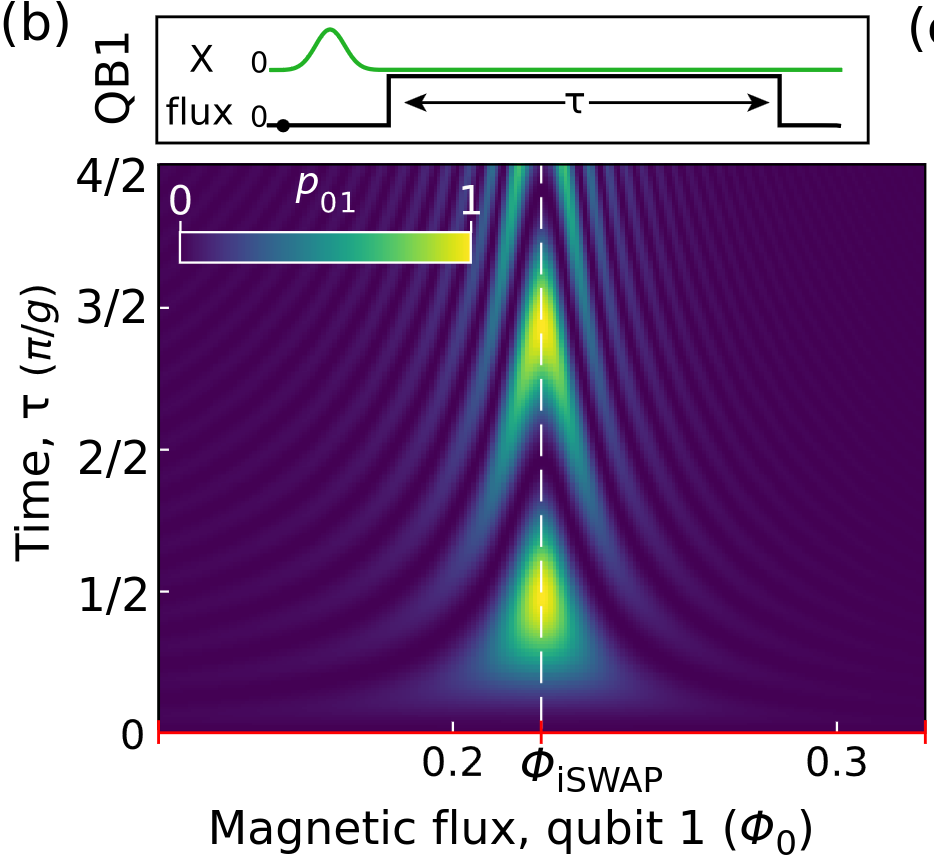
\includegraphics[width=8cm]{Two-qubits calibration/Figures/chevron_sketch.png}
    \caption{Expected plot for a two-qubits chevron.}
    \label{fig:chevron_sketch}
\end{figure}

This experiment, performed with the ZCU216 using the coded \Qibocal routines is presented in \cref{fig:nice_chevron}.

\begin{figure}[htbp]
    \centering
    \makebox[\textwidth][c]{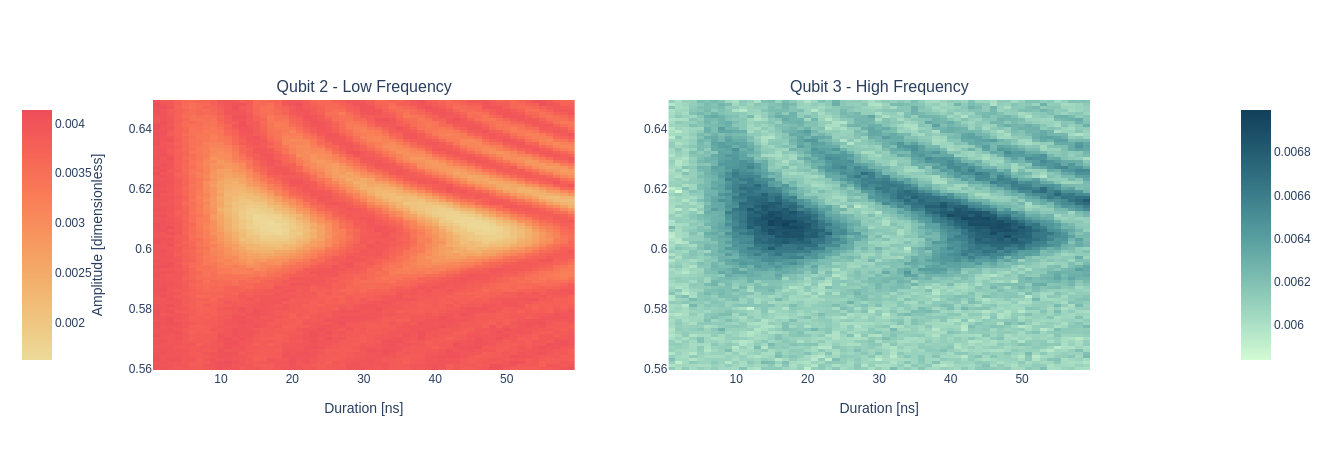
\includegraphics[width=1.3\textwidth]{Two-qubits calibration/Figures/good_chevron.png}}
    \caption{Chevron plot for CZ.}
    \label{fig:nice_chevron}
\end{figure}

The flux required for the two-qubits gate is the center one in the chevron plot, while the length of the pulse is chosen as half of the distance between two consecutive peaks at that flux (exactly as in the Rabi experiment).


\section{Flux pulse shape correction}

\begin{figure}[htbp]
    \centering
    \makebox[\textwidth][c]{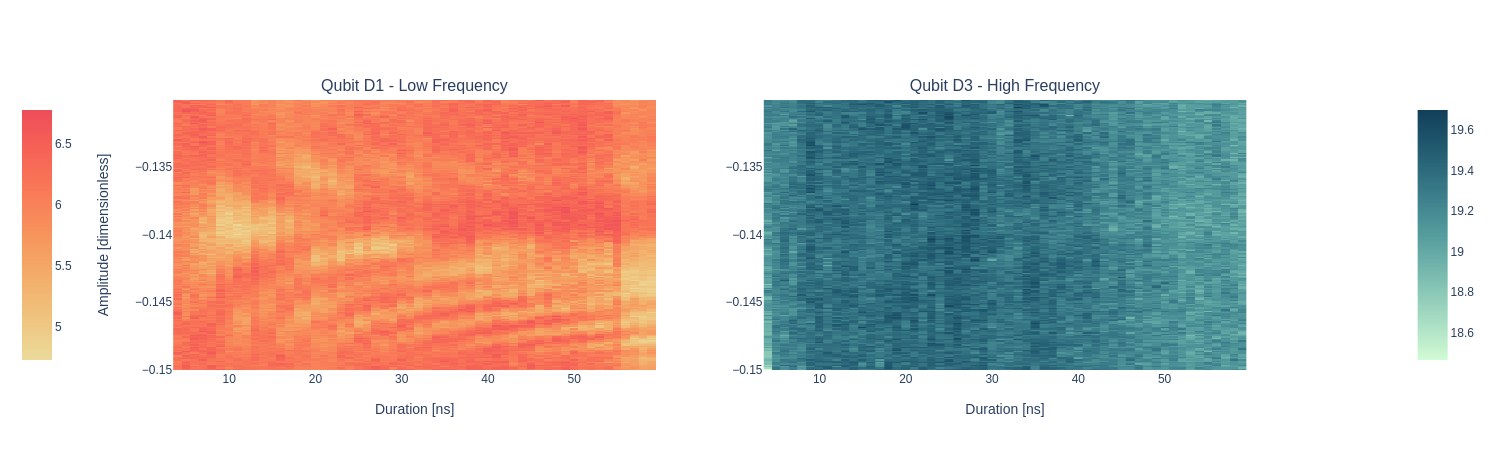
\includegraphics[width=1.3\textwidth]{Two-qubits calibration/Figures/chevron_bad.png}}
    \caption{Chevron plot for CZ. The distortion, that will be fixed in the next section, causes the asymmetry higher-lower bias. The leakage causes the chevron to not close and to not appear in the high frequency qubit.}
    \label{fig:chevron_distorted}
\end{figure}

The result of the last experiment should be exactly symmetric, as presented in \cref{fig:chevron_sketch}, but this is hardly the case.
Usually the result is much more distorted as presented in \cref{fig:chevron_distorted}, for example.

The problem in this case is the effective shape of the flux pulse.
We are now sending a rectangular pulse, with the idea that we can use it to perform a jump between two different flux values, without any transients.
In reality, the pulse gets partially deformed by the quality of the line, in particular its capacitance, that transform the pulse from a rectangular to something like what is presented in \cref{fig:rectangular_distortion}.

\begin{figure}[ht]
    \centering
    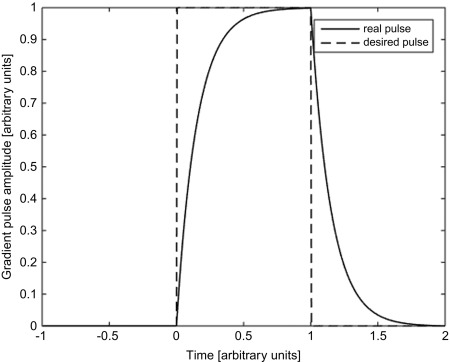
\includegraphics[width=6cm]{Two-qubits calibration/Figures/rectangular_distortion.jpg}
    \caption{Rectangular pulse distortion.}
    \label{fig:rectangular_distortion}
\end{figure}

The solution to this problem is to change the shape of the flux pulse to an ideal rectangular to something that will produce an effective rectangular~\cite{Rol2020, Ferreira2022}.
To achieve this, there are different possibilities, but the most straightforward consists in just implementing a new pulse shape and fine tune it manually using the symmetry of the chevron plot of the last experiment as figure of merit.

A sensible ansatz for the flux pulse is presented in \cref{eq:exponential-flux}.
\begin{equation}\label{eq:exponential-flux}
    y = A * \frac{(\exp(-x/\upsilon)) + g * \exp(-x/\tau)}{1+g}
\end{equation}
where basically the rectangular pulse is corrected with an initial exponential function, to counter the initial transient.





\section{Virtual phase correction}

After finding the right shape, we still have to consider a last calibration parameter: the phase.
The discussion here will be around the CZ since it presents some more problems in respect to the iSWAP, but as always everything is more or less interchangeable.

\begin{figure}[ht]
    \centering
    \makebox[\textwidth][c]{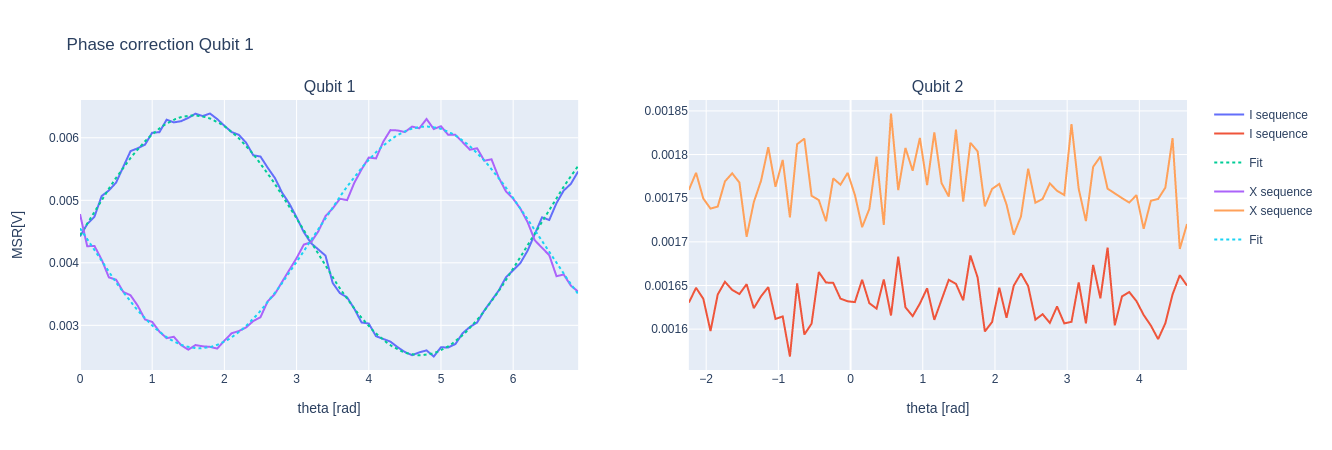
\includegraphics[width=1.3\textwidth]{Two-qubits calibration/Figures/phase_correction_1.png}}\\
    \makebox[\textwidth][c]{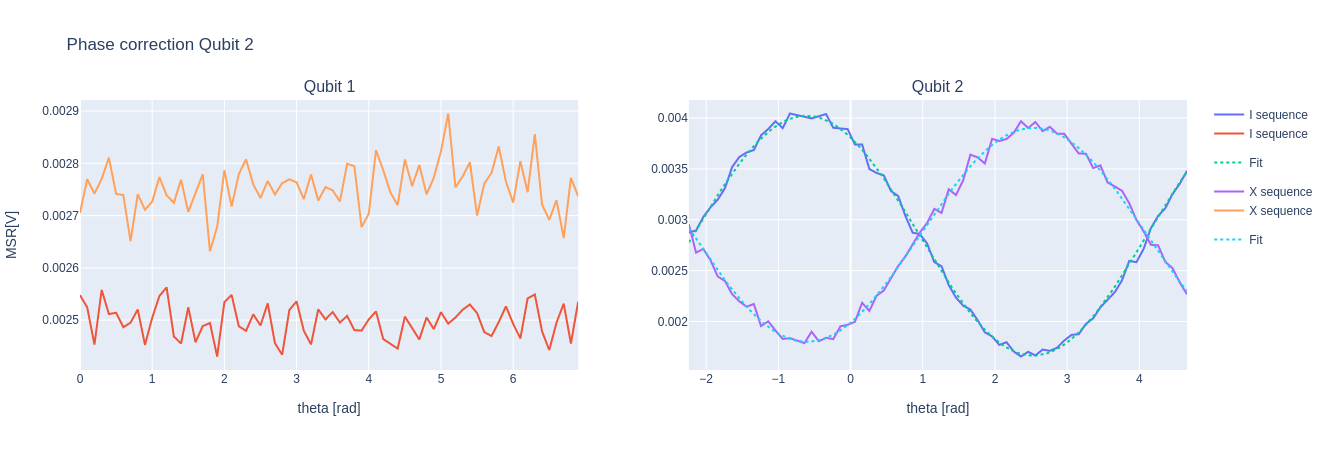
\includegraphics[width=1.3\textwidth]{Two-qubits calibration/Figures/phase_correction_2.png}}
    \caption{Calibrated virtual phase correction plot.}
    \label{fig:virtualphase}
\end{figure}

The problem is that so far we have ignored the role of the single-qubit phases acquired by tuning the qubit frequency (caused by simple time evolution). 
So, effectively we never implemented a CZ (or a iSWAP) but a CZ with the addition of a spurious relative phase between the qubits.
Critically, this phase is not dependent on the state of the control qubit, but is constant in all cases, so it will be fairly easy to implement a virtual correction once calibrated (so consider the presence of this phase for all successive pulses and measurements).

The experiment we perform is the following:
\begin{itemize}
    \item we initialize the system performing a $Y90$ pulse on the low frequency qubit and either a $I$ or a $X$ gate on the high frequency one;
    \item we apply the flux pulse for the two-qubit interaction;
    \item we undo the initial rotation on the high frequency qubit, by applying $I$ or $X$ again;
    \item we apply a $\Theta(90)$ pulse, so a rotation of $90^\circ$ around a certain angle $\theta$;
    \item we measure the two qubits;
    \item we repeat the measurement for multiple angles and for both $I$ and $X$ initial states.
\end{itemize}

Ideally, the high frequency qubit should not be affected at all by the gate, eventually some leakage to the $\ket 2$ state can be visible.

For the low frequency qubit, we should see, depending on the initial state of the control qubit, two different sinusoidal with a $90^\circ$ phase difference.
What we will actually see is presented in \cref{fig:virtualphase}.

The phase difference is not $90^\circ$ as expected but $(90+\epsilon)^\circ$ with $\epsilon$ being the virtual phase to consider for later sequences and measurements.















\chapter{Applications}

The qubits control system developed within this thesis can be used for various experiments in different quantum technology fields.
Although the integration in \Qibolab is focused on quantum computing, the final objective is to have a complete instrument able to fully control of a qubit state.
So it is possible to imagine also non-computing applications.

In any case, let's focus on the two main applications where \Qibosoq could be useful and could be used in the short term. These are:
\begin{itemize}
    \item in quantum computing, for quantum machine learning applications.
    \item in quantum sensing, in particular for the QubIT project;
\end{itemize}


\section{Quantum machine learning: determining probability density functions}
\label{sec:qml_application}

The RFSoC-based control system that was developed for this thesis has already been used in quantum machine learning applications, in particular to fit probability density functions~\cite{Robbiati2023}.

This is a relevant short-term application because even a single not-optimally-tuned qubit can be work fine.

To the reader, using a quantum computer for fitting, might seem useless. 
It is a fair doubt, but there are still situations where the analytical underlying distribution is not known and the problem cannot be efficiently solved classically.

For example, the reliable determination of probability density functions (PDF) from data samples is still an active research topic in studies of fundamental physics.\\
With quantum computing and, specifically, adiabatic evolution algorithms, it is possible to approximate the underlying distribution via a circuit-based quantum device.

Given a one-dimensional function $f(t)$ with $t\in [0, T]$, we can build a regression model by choosing an observable such that two Hamiltonans $H_0$ and $H_1$ exist and respect the condition of having their ground state energy as the two values defining the range to which the function will be bounded.

We can then interpret the regression problem as the search for a time dependent Hamiltonian such that its ground state energy evolves as $f(t)$:
\begin{equation}
    \left< H(t) \right> = f(t)
\end{equation}

The Hamiltonian can be also written in terms of a new function $s(t; \theta)$, called \textit{scheduling function}, that describes a variational circuit defined by a set of parameters $\theta$:

\begin{equation}
    H(t) = [1 - s(t; \theta)]H_0 + s(t;\theta) H_1
\end{equation}

In this way, the problem is reduced to finding the right parameters $\theta$.

The complete, schematic, procedure is at follows:

\begin{enumerate}
    \item we generate a sample of variables $\{x\}$ from a chosen distribution;
    \item we compute the empirical \textit{cumulative density function} (CDF) from the extracted samples;
    \item we select $N_{train}$ data samples such that their values match some of the evolution times controlled by $s$;
    \item we map each pair $(x_i, f_i)$ into $(\tau_i, E_i)$ with the second pair representing two generic values of the evolution time/energy of the target observable evaluated at the evolved state with $\tau = t/T$;
    \item we define a loss function to minimize as:
        \begin{equation}
            J = \frac{1}{N_{train}} \sum_{j=1}^{N_{train}} (f_j - E_j (\theta))^2
        \end{equation}
        It is important to have a monotonic regression function, eventually, we could add extra penalty terms that, increasing with $j$, would assure the monotony; 
    \item we perform a training of the parameters $\theta$ to minimize the loss function. This can be done with classic, quantum or hybrid schemes.
\end{enumerate}

\begin{figure}[ht]
    \centering
    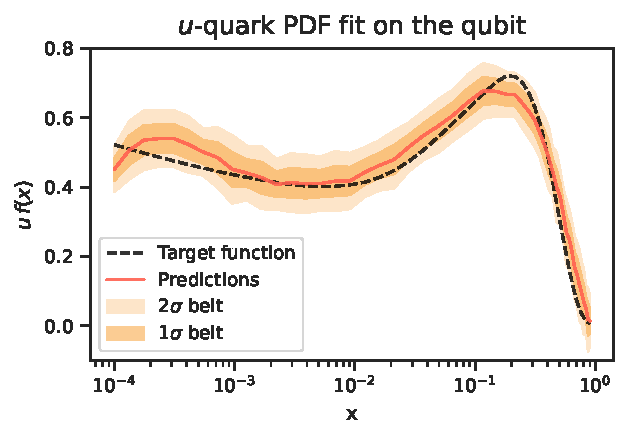
\includegraphics[width=0.6\textwidth]{Other sections/figures/qpdf.pdf}
    \caption{PDF of the $u$-quark, fitted with the QML model with a \Qibosoq-controller RFSoC.}
    \label{fig:updf}
\end{figure}

As example, we take some data samples from the NNPDF4.0~\cite{Ball2022} PDF grid.
Using a variational ansatz composed of consecutive rotations~\cite{PrezSalinas2020}, we encode the values of $x$ and proceed with the optimization minimising the MSE using the ADAM~\cite{adam} optimizer.
In this case, the optimization was done partially on classical hardware,  as a pre-training, and part on a TII single qubit device controlled by \Qibosoq.

In \cref{fig:updf}, an example of a plot obtained with this procedure is presented.
Both the expected PDF and the fitted one, with \Qibosoq and the \RFSoC, are presented.


\section{Quantum sensing applications}
\label{sec:sens_application}

For the moment, \Qibosoq has not been used in sensing applications, but it has been designed to be flexible and to support different kind of applications, from the circuits-based QML that we saw in last section to more pulse-based optimization protocols (for optimal-control, for examples) or for sensing applications.

What are the special needs of quantum sensing, from a control device / software point of view?\\
It is difficult to have a complete list of required features, but we could say that the main elements are:
\begin{itemize}
    \item extensive control of the pulses to execute (shaping, timing, frequency modulation, phases etc.);
    \item fast and precise acquisition;
    \item support for continuous measurements;
    \item good scaling properties;
    \item support for highly multiplexed systems;
\end{itemize}

\Qibosoq natively has, leveraging different \Qick functionalities, most of these characteristics.

In particular, through the Python API, the user has total control of the pulses and can both work optimizing speed and dead times, by leveraging all the pre-defined pulse shapes included in \Qibosoq, or focusing on optimal control, by defining in the client specific pulses from their IQ values.

The intrinsic characteristic of a RFSoC system give full control and flexibility on the frequency requests. 
In particular, when comparing the three currently supported Xilinx boards with the other commercial systems available for control at TII (Qblox, Quantum Machines, Zurich Instruments) the bandwidth of a single RFSoC channel (that can go above $10$ GHz) is not-comparable in respect to the standard bandwidths of $\approx200$ MHz (without local oscillators).
This speeds up \textit{incredibly} any experiment where there is the need to probe very different frequencies.

Currently, \Qick does not support continuous measurements and this reflects on \Qibosoq with the same limitation.
The problem, from the point of view of \Qick, stands in the use of memory that quickly fills the buffer size defined in FPGA logic.
Even tho this is a big limitation for sensing application, it is partially patchable through \Qibosoq.
Since \Qibosoq can be included easily in any Python client and is designed to minimize any latency, it should be possible to apply repeated measurement windows one after the other, without loosing excessive statistics in between them.\\
In any case, this issue should be taken into account and precisely measured for any real application of rare phenomena.

Regarding the scaling capabilities, the \Qick team is currently updating their firmwares so the is possible to synchronize different RFSoCs and use them collectively \textit{as a cluster-like system}.
The main \Qick developers admitted that this firmware upgrade will cause some problem in the \Qick software department: indeed the current proposed way of managing a RFSoC directly with \Qick involves a direct connection to the board, this is not possible when dealing to multiple boards at the same time.
In this problem, the \Qibosoq layout offers an easy solution: having already an external client responsible of managing communication with the board(s), it should be easy to give to it the new responsibility of splitting the program into different subsection for the different boards.

The high multiplexablity is a concept that, for qubits, has not really been under development.
However, \Qick has specific firmwares to control highly multiplexed arrays of Microwave Kinetic Inductance Detector~\cite{Magniez2022}, often referred to as MKIDs, (up to 4096 detectors with a single board). 
Although at the moment, the \Qibosoq development has been focused on qubit control, so it does not support this special firmware, it has been designed with flexibility as one of the main priority, since we knew from the start that \Qick would be upgraded independently from it and possibly without much interest in preserving backwards compatibility.\\
Thanks to this, it should not be difficult to extend support for the MKIDs firmware, although no development has yet been done in this direction.

\subsection*{Photon counter for dark matter detection}

As a theoretical example of quantum sensing application, we can take an experiment for axions detection~\cite{Dixit2021}.

In this section, we will present the code required to replicate the experiment, showcasing how a complex experiment can become trivial using the \Qibosoq API.
The experiment itself requires a hardware setup that stops me to be able to actually replicate it now, but still is a good example of how easily the implementation can become.

\begin{figure}[ht]
    \centering
    \includegraphics[width=0.6\textwidth]{Other sections/figures/dixit_setup.png}
    \caption{Hardware setup required of the axion-detection experiment.}
    \label{fig:dixit_setup}
\end{figure}

This hardware setup is presented in \cref{fig:dixit_setup} (a). 
The detection system requires a superconducting qubit (transmon) used as a bridge between a readout resonator (in the image depicted as a cavity) and an additional storage-cavity.

The idea of this detector is to exploit the Primakoff effect that should cause potential axions to convert to photons in resonance to the storage frequencies.
Now, we can use the qubit to build an extremely precise photon counter and, counting the average number of photons we may see statistically relevancy of axions existence.

We use, for this, two concepts already encountered in \cref{chap:char}:
\begin{itemize}
    \item dispersive shift;
    \item Ramsey interferometry.
\end{itemize}

We exploit the dispersive shift considering that a different photons number has a different effect on the qubit frequency.
Indeed the Hamiltonian of the system can be written as ($\omega_c$ is the cavity frequency; $a$ and $a^\dagger$ the ladder operators of the cavity; $\omega_q$ the frequency of the qubit; $\chi$ the dispersive shift and $\sigma_z$ the well-known Pauli matrix):
\begin{equation}
    H/\hbar = \omega_c a^\dagger a + \frac{1}{2} \left ( \omega_q + 2 \chi a^\dagger a \right) \sigma_z
\end{equation}
So, effectively, the qubit frequency changes with $2\chi a^\dagger a$.

To measure the different "detuning" caused by a different photons population in the storage cavity, we can use the Ramsey protocol.
In the Dixit paper~\cite{Dixit2021} that proposes this experiments, the measurement protocol works not with two \pihpulses but with a +\pihpulse and a -\pihpulse. The effect is more or less the same and it is easily coded in \Qibosoq.

Finally, to achieve exponential suppression of the readout errors, we have to repeat the measurement (the two drive pulses and the readout one) multiple consecutive times, leveraging the non-destructiveness of the measurement.
A scheme of the sequence to be executed is present in \cref{fig:dixit_sequence}.

\begin{figure}[ht]
    \centering
    \includegraphics[width=0.6\textwidth]{Other sections/figures/dixit_sequence.png}
    \caption{Overview of the pulse sequence to be executed for the axion-detection experiment.}
    \label{fig:dixit_sequence}
\end{figure}

To increase the fidelity of the experiment, a Markov-chain analysis can be employed and it already proved to be of use.
For this example, however, we will focus on the acquisition part that can be performed using \Qibosoq, while we will leave out the data processing phase.

Using the \Qibolab and \Qibosoq API, the experimental procedure  will be coded as:

\begin{lstlisting}[language=Python, numbers=left]
from qibolab import create_platform
from qibolab.pulses import PulseSequence

# we instantiate the platform (qubit + RFSoC)
platform = create_platform("platform_name")

# we initialize an empty pulse sequence
sequence = PulseSequence()

N_repetitions = 30
for i in N_repetitions:
    # we add a first pi-half pulse
    sequence.add(platform.create_RX90_pulse())
    # we add the - pi-half pulse
    sequence.add(platform.create_RX90_pulse())
    sequence[-1].amplitude = - sequence[-1].amplitude
    # we add a measurement
    sequence.add(platform.create_MZ_pulse())

# we perform the experiment, executing the sequence
results = platform.execute_pulse_sequence(sequence)
\end{lstlisting}

See that, in 21 lines (with an abundance of comments), we coded and performed the full experiment.
Clearly, some work has been hidden here, in particular the calibration parameters of the qubit, that have to been computed via the various experiments detailed in the last sections, as well as all the data processing.

This example shows how much \Qibosoq can simplify and accelerate research.




\chapter{Conclusions}

In this thesis, after presenting the main theoretical concepts and the main instruments (hardware and software) used, I focused on the characterization and calibration experiments required to fully control a superconducting quantum device.
A detailed description of all the experiments has been provided along with ideal and real plots for different scenarios.

\paragraph{Software development}

Although the explanation of these experiments is the main part of this thesis, the time spent at the Technology Innovation Institute was in large part dedicated to develop the software tools required for the experiments themselves.
This included the development of parts of \Qibolab and of \Qibosoq of which some details were given in \cref{sec:software}.

Both of these software tools are open source and are being officially presented to the research community via papers \cite{Efthymiou_2023} currently under review for the Quantum journal.

It is useful, for the purpose of better explaining my role in the development of these tools, to provide a brief description of them when I first started and when I finished the thesis.\\
When I first arrived, \Qibolab was in an alpha-testing phase and was not fully released yet.
Remember that the main idea behind \Qibolab is to support, with the same interface, multiple devices and instruments.
At that time, however, it supported only Quantum Machines devices and some Qblox devices (with outdated firmware).
My main role was to add to \Qibolab the full support of the RFSoC FPGAs compatible with the \Qick project, but I also worked in the development of the general interface, helping reaching the first stable release of the software.

For what concerns \Qibosoq, when I first arrived at TII, it was nothing but a prototype script, it was not compatible with the \Qibolab interface and therefore was not of any real use.
I developed it to the first stable release and reached a stage were all the major features supported by \Qick and \Qibolab are supported and integrated in the software.\\
The role of \Qibosoq could be critical for the research community, since it creates a connection between an open source software for control, \Qibolab, and a high-precision and economically-feasible hardware solution as the RFSoCs and \Qick.

\paragraph{Calibration experiments}

To develop and test the software solutions introduced in \Qibolab and \Qibosoq, continuous hardware testing on real qubits was required, as well as the software implementation of various calibration and characterization experiments.

In this thesis, I detailed the experiments required to fully calibrate a single qubit device, as well as the first main experiments required for two-qubit gates calibration. 
I tried to set up the calibration sections as a practical manual, so that it may be used by novice experimenters in the future.
Indeed many more experiments can be developed to increase readout and gate fidelities, but following the layout of routines detailed in this thesis will give full and acceptable control capacities on a standard superconducting qubit.
Moreover, the user of this ''manual`` will also gain a good enough knowledge on the underlying quantum-mechanical and cQED principles exploited for readout and control.
A small list of other possible calibration experiments was also provided in \cref{sec:other_possible}, to show the ''infinite`` possible number of experiments.

\paragraph{Algorithmic applications}

The RFSoC-based setup I developed during this thesis, along with the qubits I characterized and calibrated, was already used both by me and by other colleagues with no knowledge of the underlying complexity of \Qibosoq and \Qick. 
This demonstrates how relevant it is to produce a tool with a simple interface, that can be used by experimenters without needing to split focus between software and the experiment itself.

\Qibosoq has been used for algorithmic applications, of which the fitting procedure in \cref{sec:qml_application} is an example.
Moreover, it has also been used to develop a generative quantum neural network (article soon to be published).

In general, the RFSoC-based system has been proved to be as reliable as the commercial solutions and slightly faster than those, in particular for circuit-based experiments (so algorithmic applications) as presented in \cref{fig:benchmark}~\cite{qibosoq_paper, Efthymiou_2023}.

\begin{figure}[ht]
    \centering
    \includegraphics[width=\textwidth]{Other sections/figures/routines.pdf}
    \caption[Speed benchmark of a \Qibosoq system Vs. commercial alternatives]{Execution time of different qubit calibration routines on various electronics. On the left side there is the absolute times in seconds for each experiment. The ideal time (black bar) shows the minimum time the qubit needs to be affected in each experiment. On the right side the ratio between actual execution time and ideal time is shown.}
    \label{fig:benchmark}
\end{figure}


\paragraph{Outlook and quantum sensing applications}

For the moment, \Qibosoq and the RFSoC-based setup was used just for computing applications.
The software too was developed with only calibration experiments and circuits applications in mind.

To fully unlock the potential of qubits in the particle physics research world, however, and in particular to offer \Qibosoq as a complete control solution, independently from the type of final use, some development and testing is still needed.

Various experimental protocols are already been proposed to use qubits as detectors and, in any case, quantum sensing is one of the most interesting active topic of research in quantum technologies.
The experiment presented in \cref{sec:sens_application} is an example of feasible application.

Note that the majority of elements required for sensing (in general, we are always talking about pulses and measurements) are already supported, but some changes in the interface and some more features are required to make \Qibosoq a reliable tool (for example, the support for continuous acquisition modes).

Moreover, RFSoC FPGAs are not limited to the control of superconducting qubits and could be used also for different types of technologies such as photonic quantum computing (with also some hardware modification).

In the future, \Qibosoq will be extended for applications different from quantum computing and, in particular, for quantum sensing researches.


\printbibliography[heading=bibintoc]

%\appendix
%\chapter{Defining and propagating uncertainties}
%\chapter{TWPA calibration}

\end{document}
